\documentclass[a4paper,12pt]{report}
\usepackage[
  a4paper,
  left=2.2cm,
  right=2.2cm,
  top=3.5cm,
  bottom=3cm
]{geometry}

\usepackage{alltt, fancyvrb, url}
\usepackage{graphicx}
\usepackage[utf8]{inputenc}
\usepackage{float}
\usepackage[hidelinks]{hyperref}
\usepackage[table]{xcolor}
\usepackage{colortbl}


% Questo commentalo se vuoi scrivere in inglese.
\usepackage[italian]{babel}
\usepackage{cleveref}
\usepackage{titlesec}
\titleformat{\chapter}[display]
  {\centering\normalfont\huge\bfseries}{\chaptertitlename\ \thechapter}{20pt}{\Huge}
\titlespacing*{\chapter}{0pt}{-45pt}{20pt}

\graphicspath{./Resources/}

\definecolor{headerblue}{RGB}{200,220,240}

\title{Relazione per progetto Base di Dati\\``Hotel DB''}
\author{Lasse Werpers}
\date{\today}

\begin{document}

\begin{titlepage}
    \begin{center}
        \vspace*{\fill}

        \Huge{Relazione progetto per \\Base di Dati}
        \vspace{0.5cm}


        \Huge\textbf{``Hotel DB''}

        \vspace{0.5cm}
        \LARGE
        Lasse Werpers

        \vspace{0.5cm}
        \large
        %\today
        \today

        \vspace{1cm}

        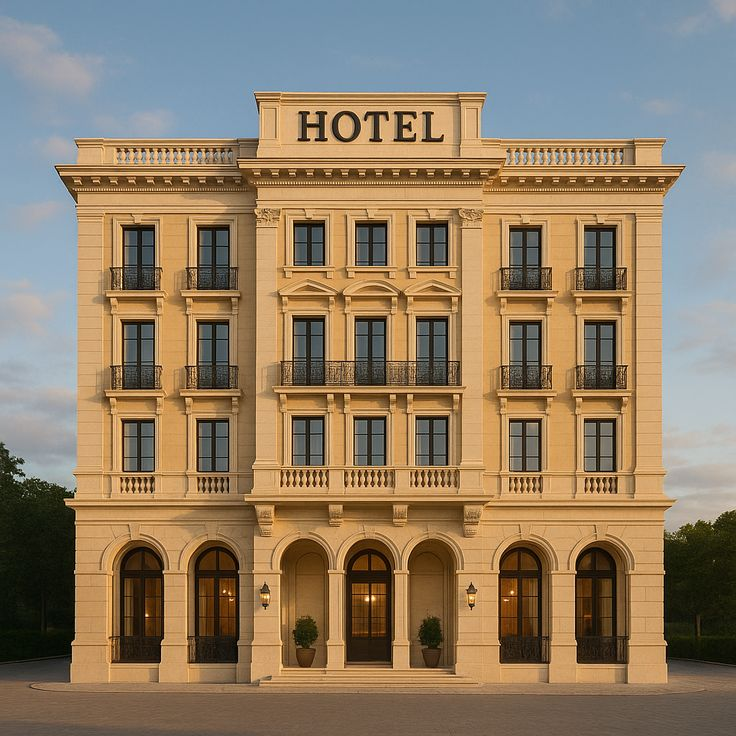
\includegraphics[width=0.7\textwidth]{../resources/HotelPicture.jpg}

        \vspace*{\fill}
    \end{center}

\end{titlepage}

\tableofcontents

\chapter{Analisi dei Requisiti}

Si vuole realizzare un database per supportare la gestione di un albergo.
Il sistema consentirà di memorizzare e gestire le informazioni principali sui clienti, sulle camere e sulle prenotazioni.
L’obiettivo è facilitare le operazioni quotidiane del personale dell’albergo, come la registrazione dei clienti, la gestione delle prenotazioni e il controllo della disponibilità delle camere.

\section{Intervista}

Si vuole realizzare una base di dati a supporto della gestione delle attività fondamentali di un albergo.
\medskip
\newline
Il sistema informativo dovrà supportare il personale dell’hotel nelle operazioni di registrazione dei clienti, gestione delle camere e delle prenotazioni, controllo dei servizi accessori, amministrazione degli utenti del sistema e produzione di report riepilogativi.
\medskip
\newline
Il sistema dovrà memorizzare i dati anagrafici dei clienti dell’hotel, registrando per ciascun cliente nome, cognome, codice fiscale e almeno un recapito tra email e numero di telefono.
Un cliente può effettuare più prenotazioni nel tempo, mentre ogni prenotazione è sempre associata a un solo cliente.
\medskip
\newline
Le camere dell’hotel sono organizzate in tipologie (ad esempio singola, doppia standard, doppia deluxe), ciascuna caratterizzata da un prezzo base, numero di posti letto, metratura ed eventuali caratteristiche aggiuntive come balcone o vista.
Ogni camera appartiene a una sola tipologia ed è identificata da un numero univoco.
Di ciascuna camera viene mantenuto lo stato corrente, che può assumere valori quali disponibile, occupata o in manutenzione.
\medskip
\newline
Il sistema deve consentire la gestione delle prenotazioni indicando il cliente, le date di check-in e check-out e applicando automaticamente eventuali sconti legati al programma loyalty del cliente.
Una prenotazione può comprendere una o più camere.
Ogni prenotazione attraversa diversi stati nel proprio ciclo di vita, quali richiesta, confermata, cancellata, check-in e check-out.
Per ciascuna prenotazione deve essere mantenuto uno storico dei cambi di stato, registrando la data e l’ora di ogni variazione.
\medskip
\newline
È previsto un programma loyalty per i clienti dell’hotel, basato su livelli (ad esempio Silver, Gold, Platinum).
Per ogni cliente viene mantenuto lo storico dei livelli loyalty posseduti nel tempo, indicando la data di inizio e di fine di ciascun livello.
Il livello loyalty applicato a una prenotazione è un’informazione derivabile sulla base dello storico del cliente nel periodo della prenotazione.
\medskip
\newline
L’hotel offre servizi accessori quali colazione, minibar o noleggio biciclette.
Ogni servizio è caratterizzato da un nome e da un prezzo unitario.
Il sistema deve consentire la registrazione delle consumazioni dei servizi, indicando data, ora, quantità e prezzo applicato.
Le consumazioni possono essere associate a una prenotazione oppure essere effettuate anche indipendentemente da un soggiorno.
\medskip
\newline
Il sistema deve inoltre registrare i pagamenti effettuati dai clienti,
sia per le prenotazioni sia per le consumazioni di servizi, indicando
l'importo, il momento in cui il pagamento avviene e il metodo
utilizzato (carta o contanti). Ai fini del calcolo del fatturato è
necessario distinguere tra il giorno in cui un servizio è erogato (o
una prenotazione si conclude) e il giorno in cui il relativo pagamento
viene effettivamente incassato: il sistema dovrà quindi supportare sia
un calcolo del fatturato per competenza (basato sull'erogazione del
servizio) sia uno per cassa (basato sull'incasso effettivo).
\medskip
\newline
Il sistema deve gestire gli utenti interni che accedono all’applicazione.
Ogni utente è identificato da credenziali di accesso e può ricoprire uno o più ruoli tra amministratore, receptionist, addetto alla contabilità e addetto alla manutenzione.
I ruoli determinano implicitamente le operazioni che l’utente è autorizzato a svolgere all’interno del sistema.
\medskip
\newline
Infine, il sistema deve supportare la produzione di report di base, tra cui l’elenco delle camere disponibili in un determinato intervallo di date, l’elenco delle prenotazioni per una data specifica e il calcolo del fatturato giornaliero derivante da prenotazioni concluse e consumazioni registrate.

\newpage
\section{Estrazione dei concetti principali}

\begin{table}[h]
    \centering
    \rowcolors{2}{gray!10}{white}
    \begin{tabular}{|l|p{7cm}|l|}
        \hline
        \rowcolor{headerblue}
        \textbf{Termine}  & \textbf{Descrizione}                                                    & \textbf{Sinonimi} \\
        \hline
        Cliente           & Persona che effettua prenotazioni presso l’hotel                        & Ospite            \\
        Prenotazione      & Richiesta di soggiorno per uno o più periodi e camere                   & Booking           \\
        Camera            & Unità abitativa dell’hotel                                              & Stanza            \\
        TipologiaCamera   & Categoria di camere con caratteristiche comuni                          & Tipo camera       \\
        StatoPrenotazione & Stato logico di una prenotazione nel suo ciclo di vita                  & .........         \\
        LivelloLoyalty    & Livello del programma fedeltà                                           & Tier              \\
        Servizio          & Prestazione accessoria offerta dall’hotel                               & Extra             \\
        Consumo           & Utilizzo di un servizio da parte di un cliente                          & Consumazione      \\
        Pagamento         & Transazione di incasso relativa a una prenotazione o a una consumazione & Incasso           \\
        Utente            & Persona che utilizza il sistema informativo                             & Operatore         \\
        Ruolo             & Insieme di permessi associati a un utente                               & Profilo           \\
        \hline
    \end{tabular}
    \caption{Glossario dei concetti principali}
\end{table}

\subsection{Riformulazione dei requisiti}
A seguito della lettura e comprensione dei requisiti, si procede redigendo un testo che ne
riassuma tutti i concetti e in particolare ne estragga quelli principali eliminando le ambiguità
sopra rilevate:
\vspace{8mm}

Per ogni \textbf{cliente} dell’hotel vengono memorizzati i dati anagrafici principali e i recapiti.
Un cliente può effettuare \textbf{più prenotazioni nel tempo}, mentre ogni prenotazione è sempre riferita a un solo cliente.
\medskip
\newline
L’hotel dispone di \textbf{camere}, ciascuna identificata univocamente e appartenente a una sola \textbf{tipologia di camera}.
Le tipologie di camera sono caratterizzate da un prezzo base e da attributi descrittivi.
Ogni camera possiede uno \textbf{stato corrente} che ne indica la disponibilità.
\medskip
\newline
Le \textbf{prenotazioni} sono caratterizzate da un periodo di soggiorno e possono comprendere \textbf{una o più camere}.
Ogni prenotazione attraversa diversi stati nel tempo; di ciascun cambiamento di stato viene mantenuto uno storico con data e ora.
\medskip
\newline
Il sistema gestisce un \textbf{programma loyalty} basato su livelli.
Ogni cliente può possedere più livelli loyalty nel tempo, ciascuno valido per un intervallo temporale.
Il livello loyalty applicato a una prenotazione è un’informazione derivata dallo storico del cliente.
\medskip
\newline
L’hotel offre \textbf{servizi accessori}, che possono essere consumati dai clienti durante o al di fuori di un soggiorno.
Ogni consumo viene registrato indicando servizio, data, quantità e prezzo applicato.
\medskip
\newline
Ogni prenotazione e ogni consumazione può essere associata a un
\textbf{pagamento}, che ne registra importo, momento e metodo (carta o
contanti). Il pagamento è considerato unico e contestuale all'evento a
cui si riferisce.
\medskip
\newline
Il sistema informativo è utilizzato da \textbf{utenti interni}, ciascuno dei quali può ricoprire \textbf{più ruoli} operativi.


\section{Requisiti}

L'applicazione deve risultare facile da apprendere anche per persone che non si affacciano regolarmente con il mondo informatico.


\subsubsection{Requisiti funzionali}
\begin{itemize}
    \item Gestione Clienti:
          \begin{itemize}
              \item  Il sistema deve consentire la \textbf{registrazione di un nuovo cliente}, memorizzandone i dati anagrafici e almeno un recapito tra email o numero di telefono.
              \item Il sistema deve consentire la \textbf{modifica e la consultazione} dei dati di un cliente.
              \item Il sistema deve consentire la \textbf{visualizzazione dello storico delle prenotazioni} associate a un cliente.
          \end{itemize}
    \item Programma Loyalty:
          \begin{itemize}
              \item  Il sistema deve consentire la \textbf{definizione dei livelli Loyalty} disponibili.
              \item Il sistema deve consentire la \textbf{gestione dello storico dei livelli Loyalty}
              \item Il sistema deve consentire il \textbf{calcolo automatico dello sconto Loyalty} applicabile a una prenotazione in base al livello del cliente nel periodo considerato.
          \end{itemize}
    \item Gestione Tipologie e Camere:
          \begin{itemize}
              \item  Il sistema deve consentire la \textbf{creazione, modifica e consultazione delle tipologie di camera}, specificandone le caratteristiche principali.
              \item Il sistema deve consentire \textbf{l'inserimento e la gestione delle singole camere}, assiociandole a una tipologia.
              \item Il sistema deve consentire l'\textbf{aggiornamento e la gestione dello stato di una camera} (disponibile, occupata, in manutenzione).
          \end{itemize}
    \item Gestione Tipologie e Camere:
          \begin{itemize}
              \item  Il sistema deve consentire la \textbf{creazione, modifica e consultazione delle tipologie di camera}, specificandone le caratteristiche principali.
              \item Il sistema deve consentire \textbf{l'inserimento e la gestione delle singole camere}, assiociandole a una tipologia.
              \item Il sistema deve consentire l'\textbf{aggiornamento e la gestione dello stato di una camera} (disponibile, occupata, in manutenzione).
          \end{itemize}
    \item Gestione Prenotazioni:
          \begin{itemize}
              \item Il sistema deve consentire la \textbf{creazione di una prenotazionej}, specificando cliente, date di check-in e check-out.
              \item Il sistema deve consentire l'\textbf{associazione di una o più camere} a una prenotazione.
              \item Il sistema deve consentire la \textbf{modifica o cancellazione di una prenotazione}, nel rispetto del suo stato corrente.
              \item Il sistema deve consentire la \textbf{ gestione degli stati di una prenotazione} (richiesta, confermata, cancellata, check-in, check-out
              \item Il sistema deve mantenere lo \textbf{storico dei cambi di stato} di ogni prenotazione, con data e ora.
              \item Il sistema deve consentire la \textbf{registrazione del pagamento} contestualmente alla creazione di una prenotazione.
          \end{itemize}
    \item Gestione Servizi e Consumi:
          \begin{itemize}
              \item Il sistema deve consentire la \textbf{definizione dei servizi accessori} offerti dall'hotel e dal relativo prezzo unitario.
              \item Il sistema deve consentire la \textbf{registrazione delle consumazioni dei servizi}, indicando data, quantità e prezzo applicato.
              \item Il sistema deve consentire l'\textbf{associazione di una consumazione a una prenotazione}, quando presente.
              \item Il sistema deve consentire la \textbf{registrazione di consumazioni anche senza una prenotazione associata}
              \item Il sistema deve consentire la \textbf{registrazione del pagamento} contestualmente alla registrazione di una consumazione.
          \end{itemize}

    \item Gestione Utenti e Ruoli:
          \begin{itemize}
              \item Il sistema deve consentire la \textbf{creazione e gestione degli utenti} che accedono all'applicazione.
              \item Il sistema deve consentire l'\textbf{assegnazione di uno o più ruoli a ciascun utente}.
              \item Il sistema deve consentire la \textbf{consultazione dei ruoli associati a un utente}.
          \end{itemize}
    \item Reportistica:
          \begin{itemize}
              \item Il sistema deve consentire la \textbf{visualizzazione delle camere disponibili} in un determinato intervallo di date.
              \item Il sistema deve consentire la \textbf{visualizzazione delle prenotazioni} relative a una data specifica.
              \item Il sistema deve consentire il \textbf{calcolo del fatturato giornaliero per competenza}, includendo prenotazioni concluse e consumazioni registrate.
              \item Il sistema deve consentire il \textbf{calcolo degli incassi giornalieri per cassa}, basato sui pagamenti effettivamente registrati in una data.
          \end{itemize}
\end{itemize}

\subsubsection{Requisiti non funzionali}
\begin{itemize}
    \item L’applicazione deve risultare facile da apprendere anche per persone che non si affacciano regolarmente con il mondo informatico.
    \item Il software:
          \begin{itemize}
              \item deve essere eseguibile in modo relativamente fluido.
              \item deve essere compatibile con una varia gamma di hardware e sistemi operativi (Linux, Windows e MacOS).
          \end{itemize}
    \item L'applicativo dovrà essere più efficente possibile.
\end{itemize}

\chapter{Progettazione Concettuale}

\section{Schema ER Finale}

\begin{figure}[H]
    \centering
    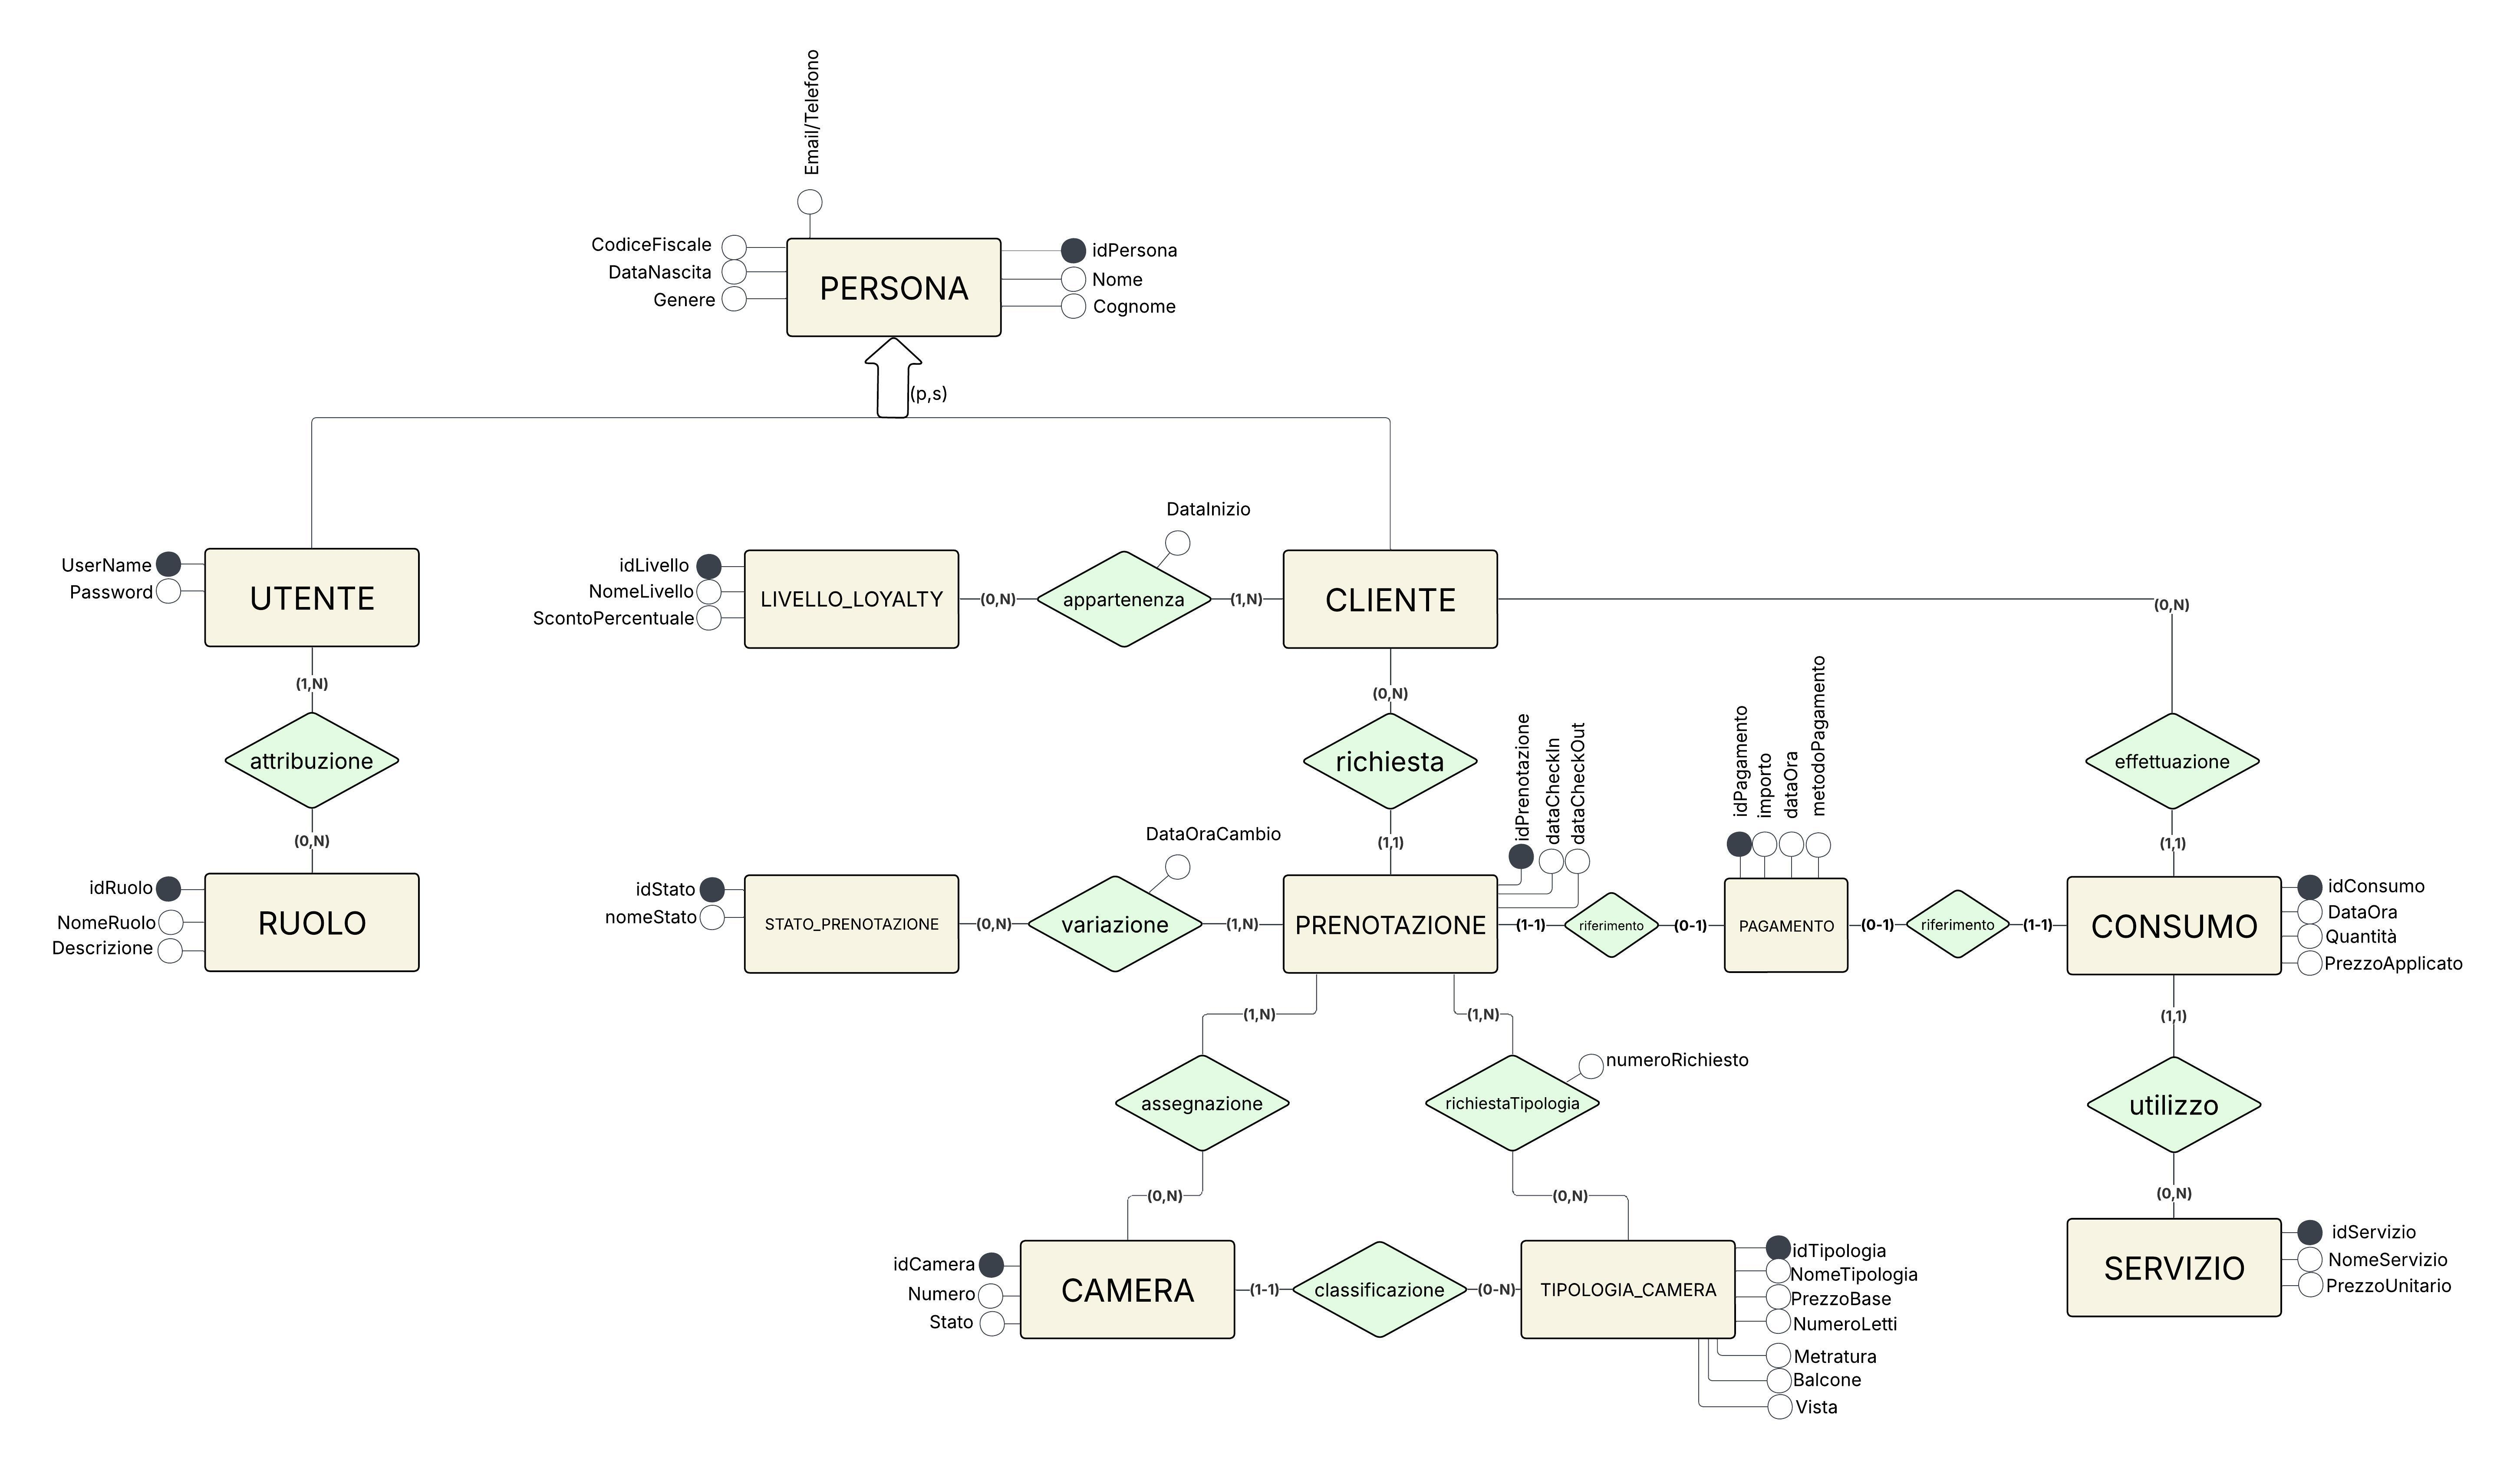
\includegraphics[angle=0,width=0.95\textwidth]{../resources/HotelDB_ER_Finale.jpeg}
    \caption{Schema E/R Finale}
\end{figure}

\newpage

\section{Spiegazione dello schema}
\subsection{Generalizzazione di \textit{PERSONA}}
Le entità di \textbf{UTENTE} e \textbf{CLIENTE} sono la generalizzazione di una entità \textbf{PERSONA}, identificata tramite un codice univoco (non si utilizza il codice fiscale per evitare problemi di omocodia).
\newline
Tali soggetti condividono un insieme di informazioni anagrafiche comuni, ma presentano comportamenti e responsabilità diverse.
\newline
Per evitare ridondanze e migliorare la chiarezza concettuale, si è introdotta l’entità \textbf{PERSONA}, generalizzata nelle entità \textbf{CLIENTE} e \textbf{UTENTE}.
\medskip
\newline
La generalizzazione è stata modellata come:
\begin{itemize}
    \item \textbf{parziale}, in quanto non tutte le persone devono necessariamente essere clienti o utenti del sistema;
    \item \textbf{sovrapposta}, poiché una stessa persona può ricoprire entrambi i ruoli (ad esempio un dipendente che soggiorna presso l’hotel).
\end{itemize}
Questa scelta consente di separare correttamente le responsabilità dei soggetti mantenendo al contempo una struttura flessibile ed estendibile.

\begin{figure}[H]
    \centering
    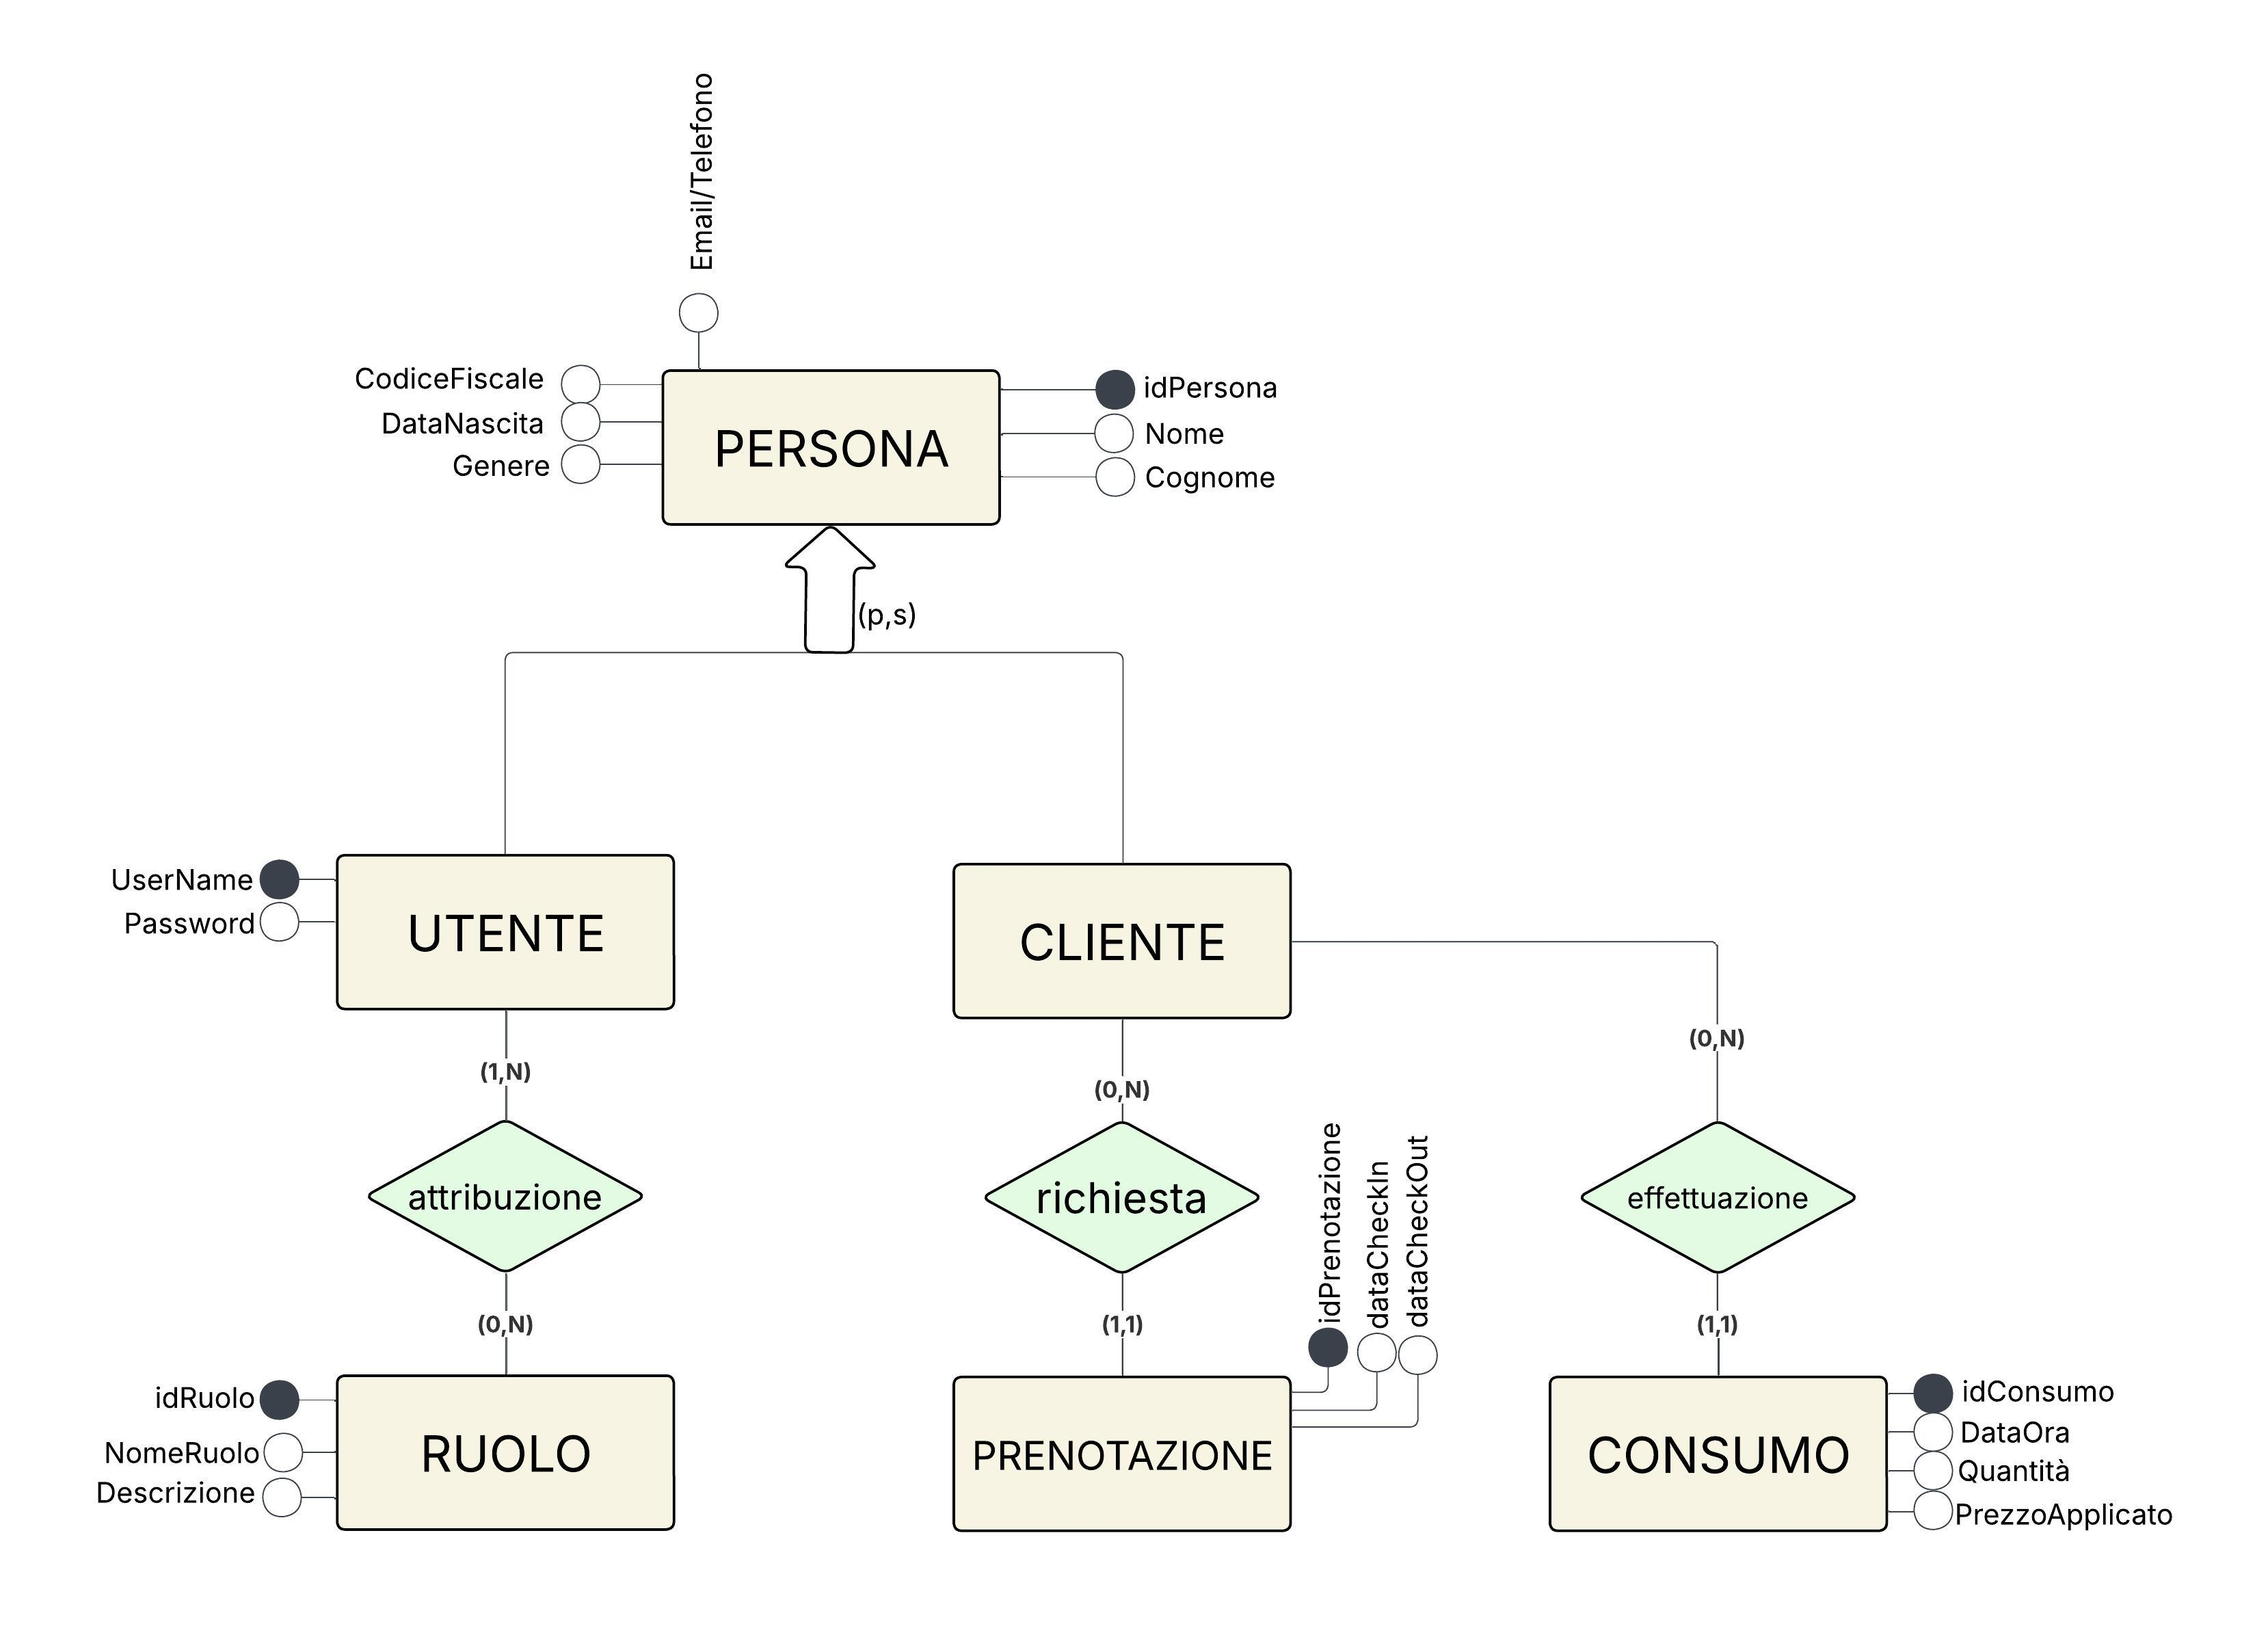
\includegraphics[angle=0,width=0.75\textwidth]{../resources/ER/HotelDB_ER_GeneralizzazionePersona.jpeg}
    \caption{Schema E/R con le principali entità per mostrare la generalizzazione inserita nel progetto}
\end{figure}

\newpage

\subsection{Ambiguità Temporale PRENOTAZIONI-CAMERE}
\label{sec:AmbiguitaPrenotazioni}
Una \textbf{PRENOTAZIONE} può comprendere una o più \textbf{CAMERE}, mentre una \textbf{CAMERA} può essere associata a più \textbf{PRENOTAZIONI} nel tempo.\medskip
\newline
Gli attributi \textbf{dataCheckIn} e \textbf{dataCheckOut} sono stati trattati come attributi della entità \textbf{PRENOTAZIONE} e non dell'associazione \textbf{assegnazione}. Ciò comporta che le CAMERE assegnate a una PRENOTAZIONE devono essere tutte nello stesso periodo.
\newline
Per prenotare \textit{n} camere diverse per \textit{m} periodi diversi serviranno \textit{m} prenotazioni separate (anche il caso in cui una sola delle \textit{n} camere della prenotazione ha il checkIn 1 gg prima o 1 gg dopo).\medskip
\newline
Questa relazione è stata modellata come associazione molti-a-molti. Tuttavia, tale modellazione introduce una potenziale ambiguità: una stessa camera \emph{non può essere assegnata a prenotazioni sovrapposte temporalmente.}
Questo vincolo non è rappresentabile graficamente mediante sole cardinalità nello schema E/R e dovrà quindi essere gestito tramite controlli software.

\begin{figure}[H]
    \centering
    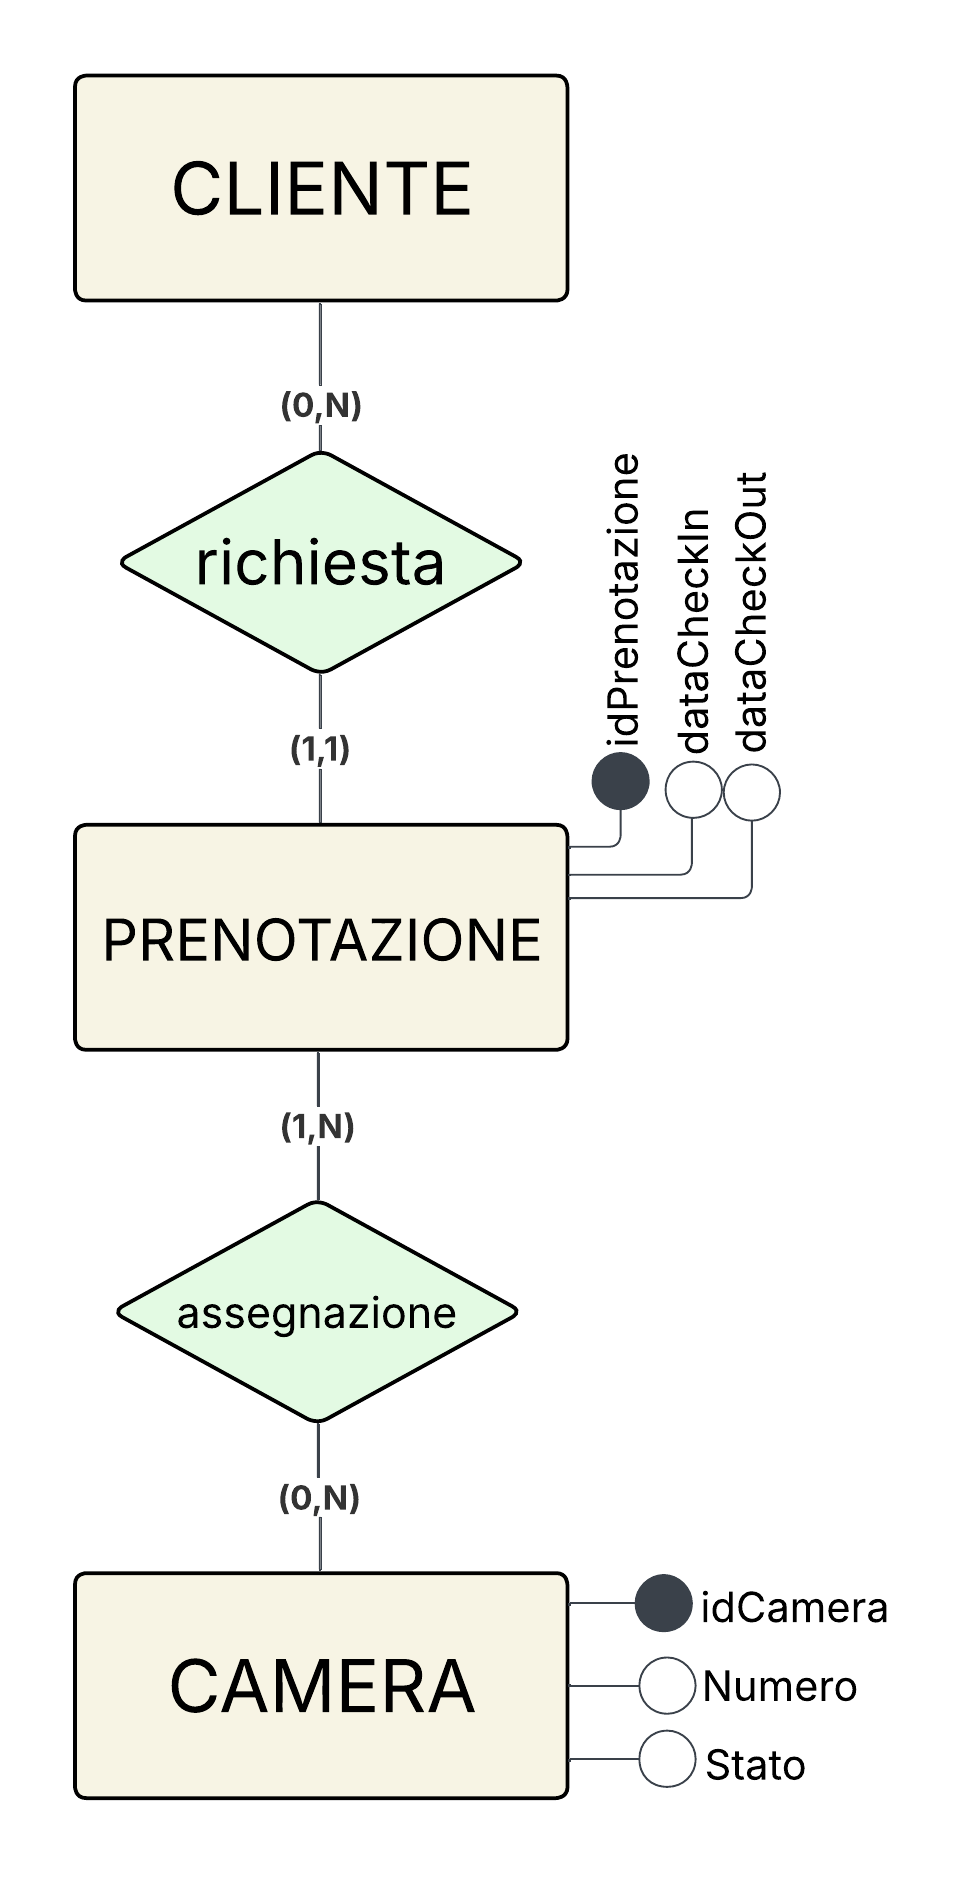
\includegraphics[angle=0,width=0.40\textwidth]{../resources/ER/HotelDB_ER_Prenotazione-Camera.png}
    \caption{Schema E/R con associazione Prenotazione-Camera molti-a-molti}
\end{figure}

\subsection{Storico degli Stati di una PRENOTAZIONE (variazione)}
L'associazione \textbf{variazione} tra \textbf{PRENOTAZIONE} e \textbf{STATO\_PRENOTAZIONE} è stata modellata come \textit{molti-a-molti}, con attributo \textbf{DataOraCambio} e cardinalità (1,N) sul lato \textbf{PRENOTAZIONE} --- ogni prenotazione attraversa almeno un cambio di stato --- e (0,N) sul lato \textbf{STATO\_PRENOTAZIONE}, poiché ciascuno stato può essere associato a molte prenotazioni nel tempo.\medskip
\newline
Non esiste, nello schema, un attributo \textbf{StatoAttuale} direttamente su \textbf{PRENOTAZIONE}: lo stato corrente di una prenotazione è un'informazione \textit{derivabile} dallo storico delle variazioni, corrispondendo alla riga con \textbf{DataOraCambio} più recente per quella prenotazione. Introdurre un attributo separato per lo stato corrente duplicherebbe un'informazione già ricavabile dallo storico, violando lo stesso criterio di \textbf{minimalità}.
\newline
Nella fase di \textit{Progettazione Logica} verrà quindi fatta un'analisi se inserire la ridondanza oppure no.\medskip
\newline
È stato inoltre confermato, come regola operativa e non come vincolo rappresentabile nello schema E/R, che la creazione di una nuova \textbf{PRENOTAZIONE} comporta automaticamente l'inserimento di una riga in \textbf{variazione} con stato iniziale ``Requested'': questo garantisce che ogni prenotazione abbia sempre almeno una variazione associata, coerentemente con la cardinalità (1,N) sopra indicata. Tale automatismo verrà tradotto in fase di Progettazione Logica come parte dell'operazione ``Crea prenotazione'' (\cref{tab:operazioni}), non richiede modifiche allo schema concettuale.

\begin{figure}[H]
    \centering
    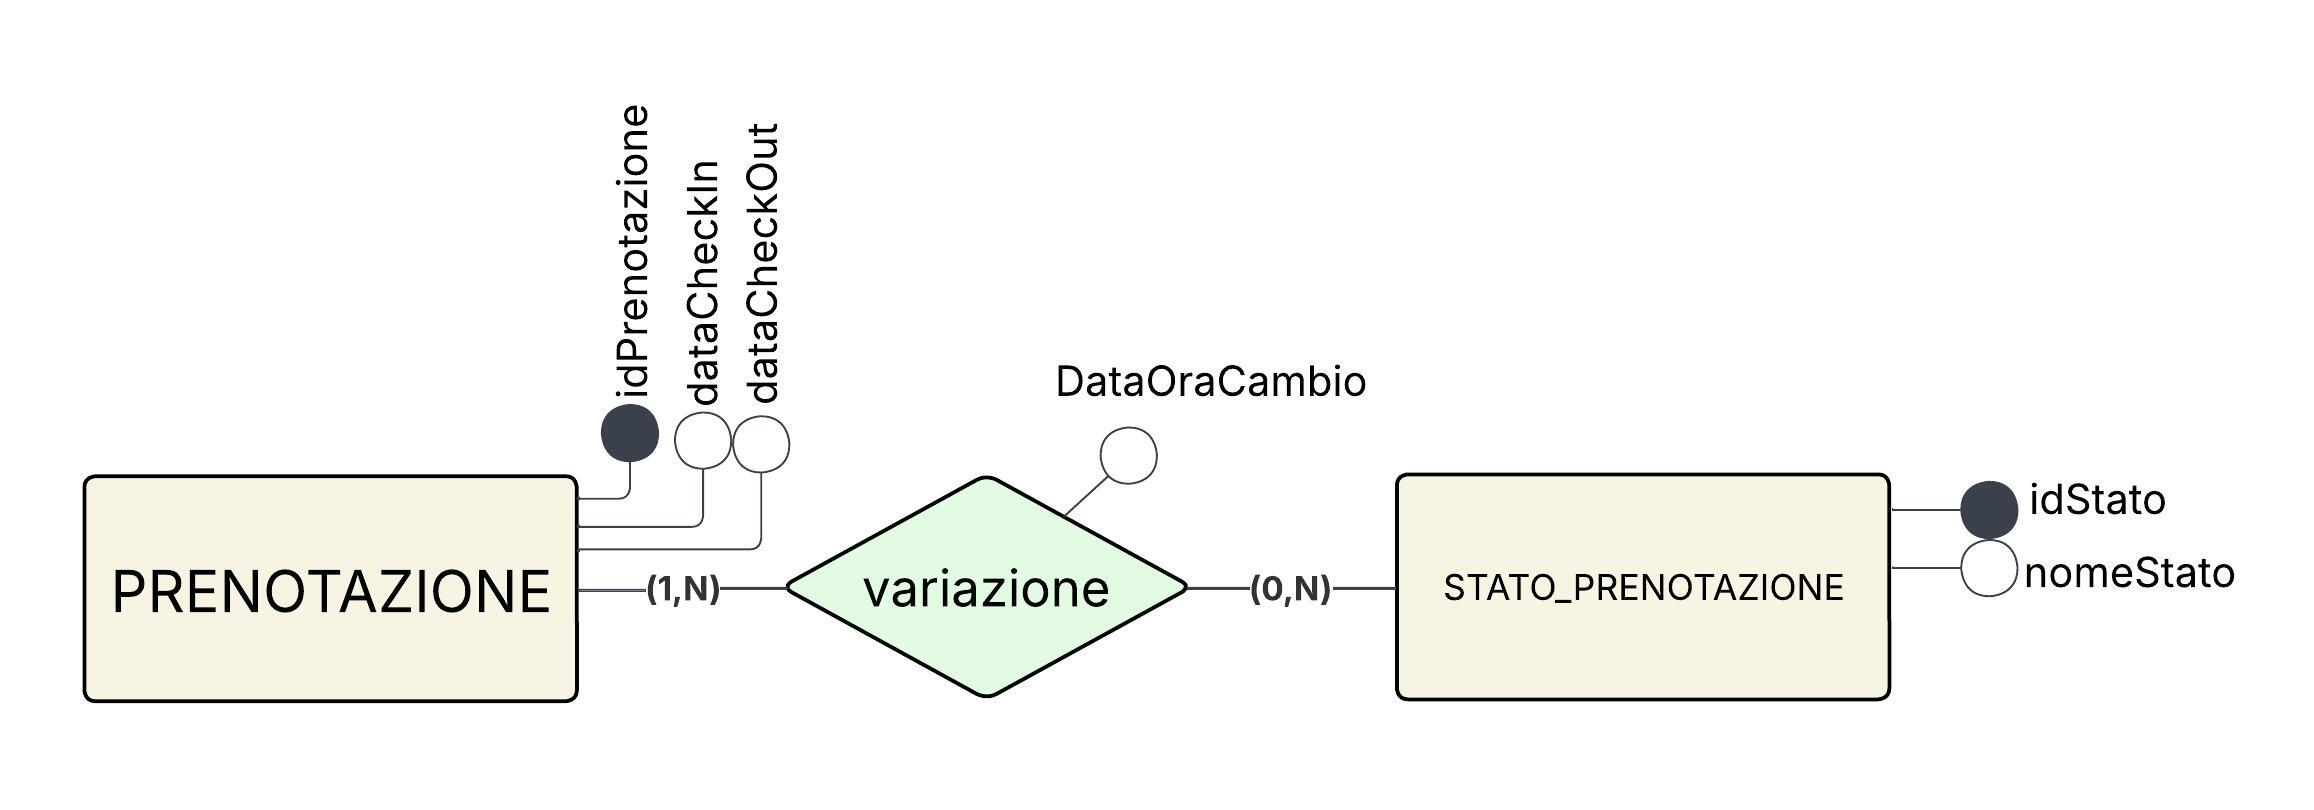
\includegraphics[angle=0,width=\textwidth]{../resources/ER/HotelDB_ER_StatoPrenotazione.jpeg}
    \caption{Schema E/R con associazione Prenotazione-Camera molti-a-molti}
\end{figure}

\newpage

\subsection{PRENOTAZIONE - CAMERA - TIPOLOGIA\_CAMERA}
L'associazione tra \textbf{PRENOTAZIONE} e \textbf{CAMERA} è già stata discussa nel paragrafo \texttt{\hyperref[sec:AmbiguitaPrenotazioni]{Ambiguità temporale PRENOTAZIONI-CAMERE}}.
\medskip
\newline
Ogni \textbf{CAMERA} è classificata da una \textbf{TIPOLOGIA\_CAMERA}, ciascuna caratterizzata da specifiche proprietà commerciali e descrittive.\medskip
\newline
Si è scelto di modellare \textbf{TIPOLOGIA\_CAMERA} come entità separata e non come generalizzazione, in quanto le differenze tra le tipologie non riguardano la struttura concettuale delle camere, ma esclusivamente attributi configurabili come prezzo base o caratteristiche.
software.\medskip
\newline
L'associazione è stata modellata \textit{uno-a-molti} perché una \textbf{CAMERA} può essere classificata da una \textbf{TIPOLOGIA\_CAMERA} e una \textbf{TIPOLOGIA\_CAMERA} può essere attribuita a molte \textbf{CAMERE}.
\medskip
\newline
L'associacione \texttt{richiestaTipologia} è stata aggiunta in seguito ad analisi nella fase \textit{ProgettazioneLogica} in quanto nel momento della prenotazione si può fare richiesta di (1-N) tipologieCamera e ogni richiesta può riguardare \textit{numeroRichiesto} camere per tipologia. Una \textbf{TIPOLOGIA\_CAMERA} può essere riferita a (0-N) \textbf{PRENOTAZIONI}.

\begin{figure}[H]
    \centering
    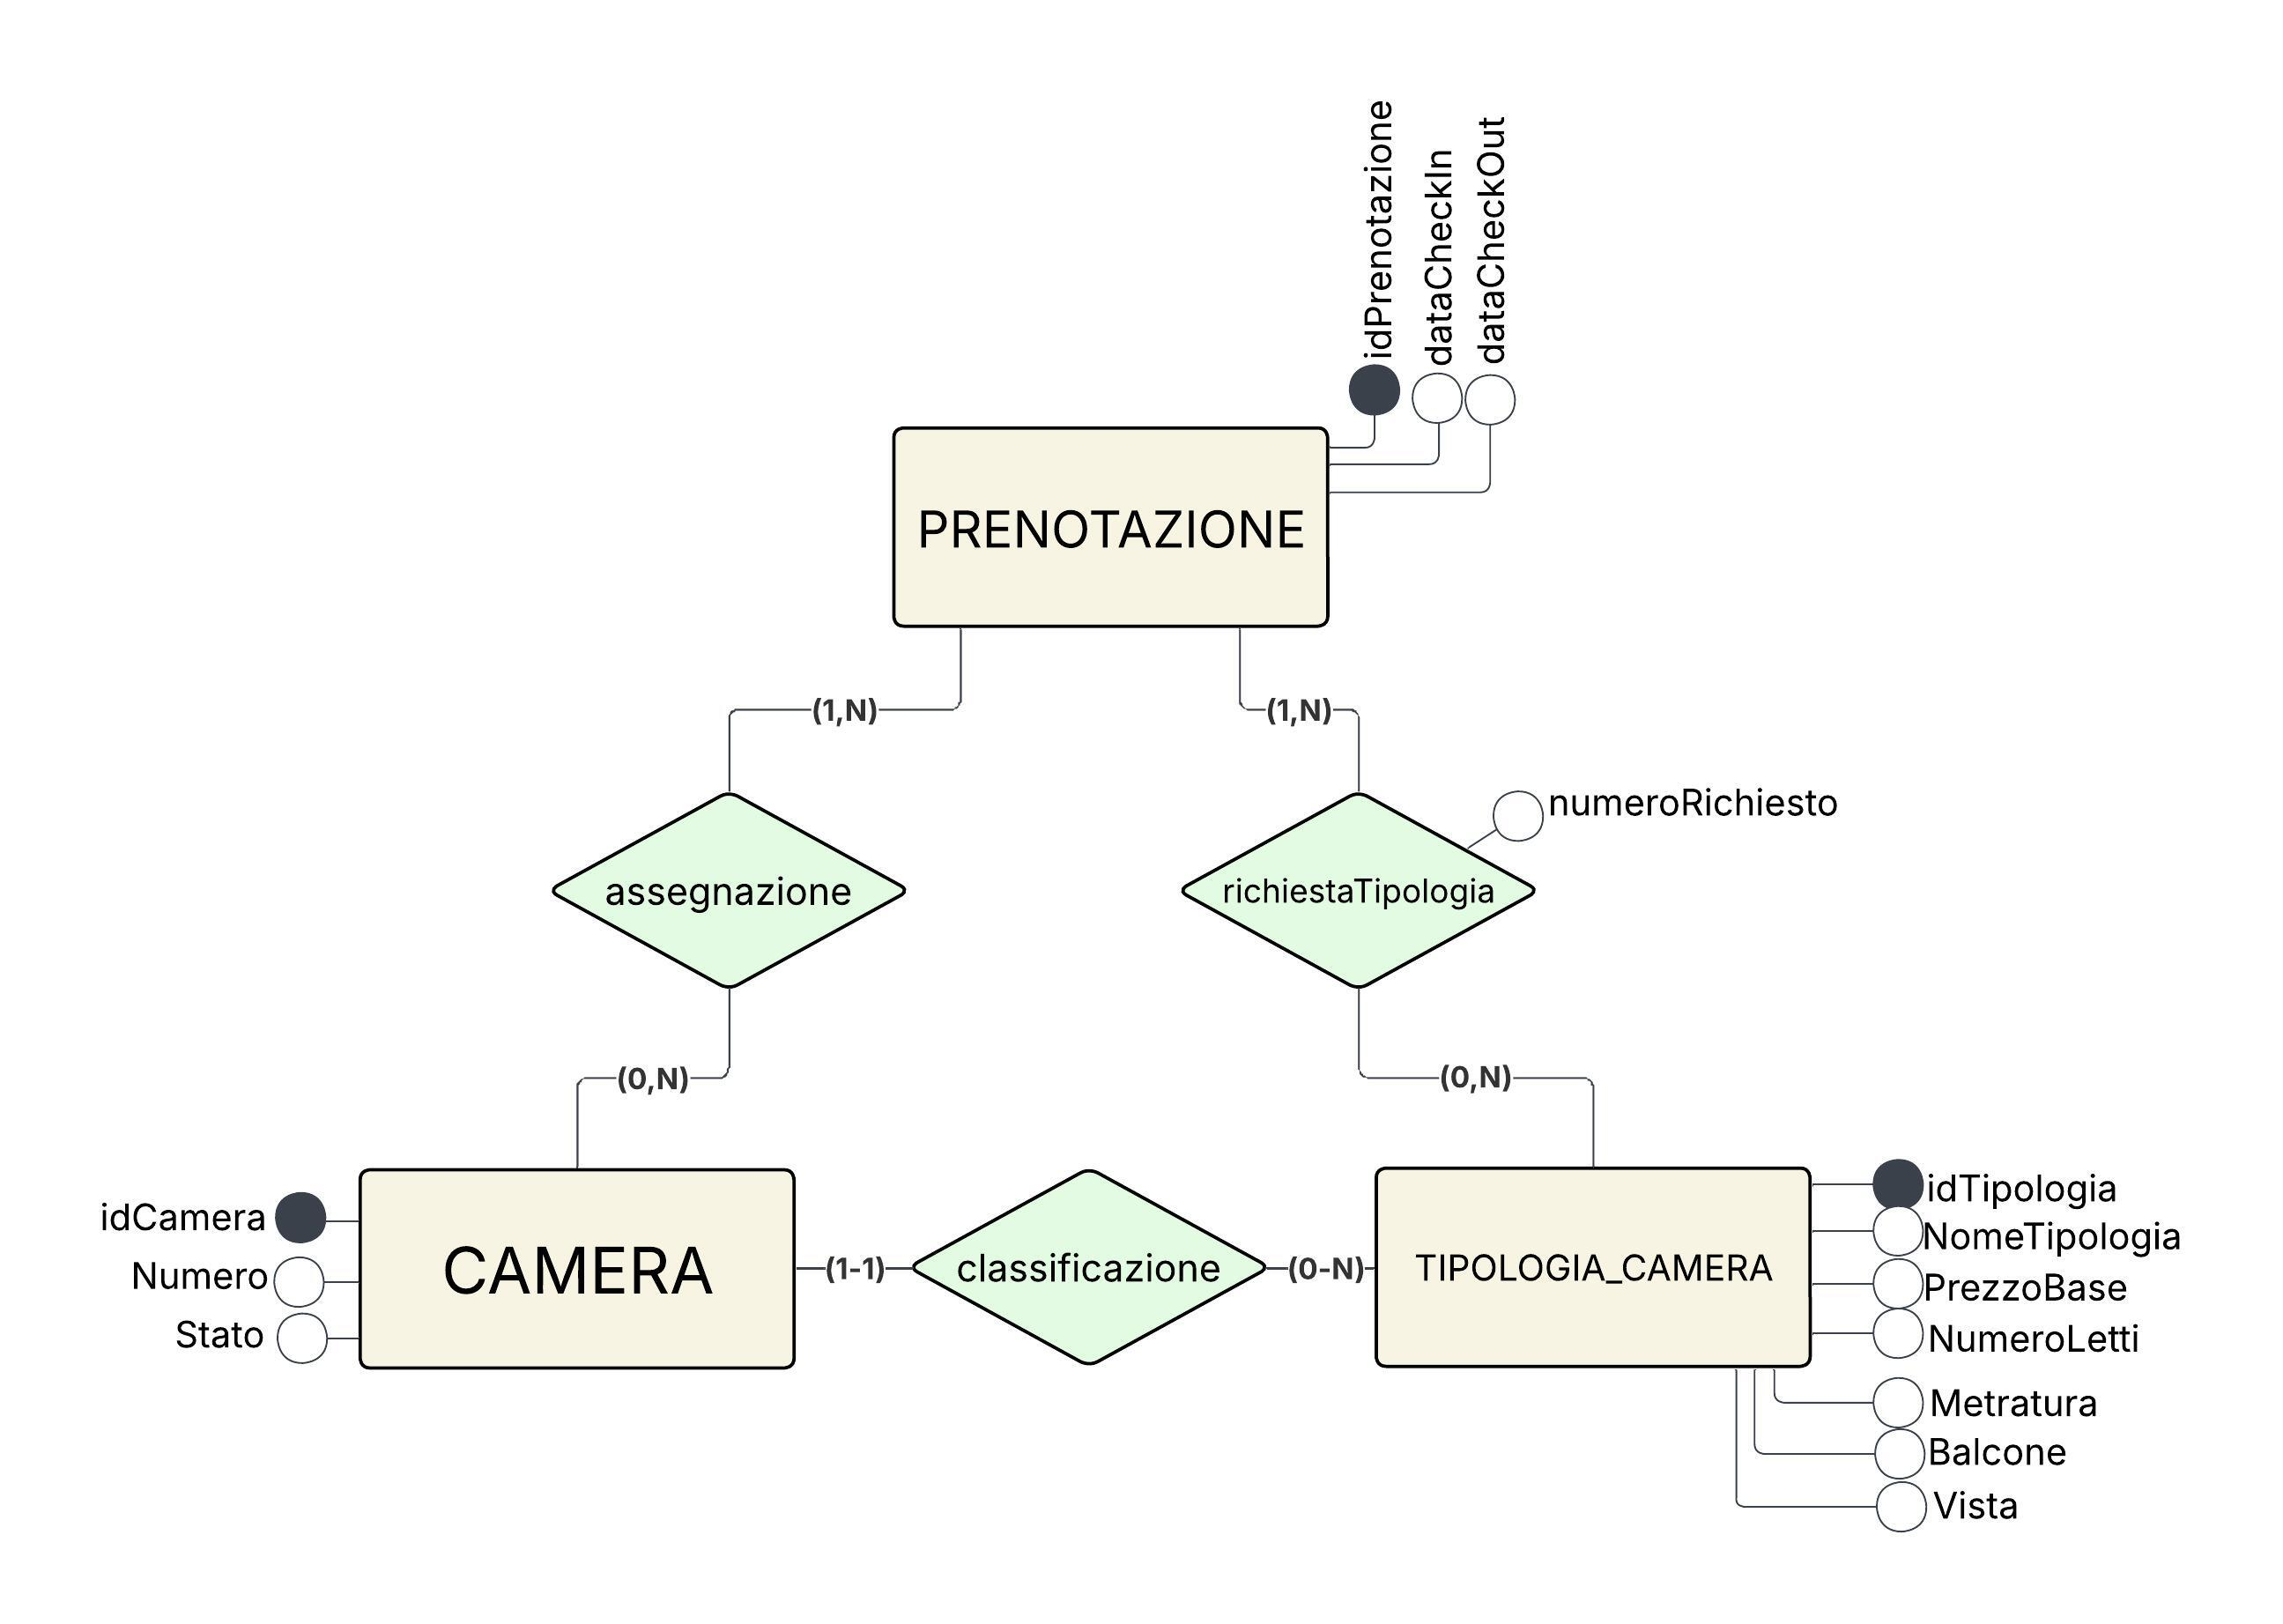
\includegraphics[angle=0,width=0.85\textwidth]{../resources/ER/HotelDB_ER_Prenotazione-Camera-TipologiaCamera.jpeg}
    \caption{Schema E/R per mostrare associazione tra PRENOTAZIONE, CAMERA e TIPOLOGIA\_CAMERA}
\end{figure}

\newpage

\subsection{Storico dei Livelli Loyalty}

L'associazione \textbf{appartenenza} tra \textbf{CLIENTE} e \textbf{LIVELLO\_LOYALTY} presenta l'attributo \textbf{DataInizio}, che indica da quando un cliente possiede un determinato livello. Non è stato invece introdotto un attributo \textbf{DataFine} esplicito.\medskip
\newline
Si è scelto di non rappresentare la data di fine nello schema perché è un'informazione \textit{derivabile}: dato lo storico dei livelli di un cliente ordinato per \textbf{DataInizio}, la data di fine di un livello coincide con la data di inizio del livello immediatamente successivo, se esiste; se il livello è quello attualmente posseduto dal cliente, non ha (ancora) una data di fine.\medskip
\newline
Introdurre comunque un attributo \textbf{DataFine} avrebbe reso lo schema ridondante, poiché il suo valore sarebbe interamente determinabile da dati già presenti (violando il criterio di \textbf{minimalità} richiesto per uno schema concettuale di qualità), a fronte del solo vantaggio di semplificare leggermente alcune interrogazioni. La derivazione verrà quindi calcolata in fase di traduzione delle operazioni in query SQL (tipicamente con una sotto-interrogazione correlata o una funzione finestra come \texttt{LEAD}), e non richiede modifiche allo schema concettuale.
\newline
È stato inoltre confermato, come regola operativa e non come vincolo
rappresentabile nello schema E/R, che la creazione di un nuovo
\textbf{CLIENTE} comporta automaticamente l'inserimento di una riga in
\textbf{appartenenza} con il livello loyalty base e \texttt{DataInizio}
pari alla data di registrazione: questo garantisce che ogni cliente abbia
sempre almeno una appartenenza associata, coerentemente con la
cardinalità (1,N) sopra indicata. Tale automatismo verrà tradotto in fase
di Progettazione Logica come parte dell'operazione ``Registra nuovo
cliente'' (\cref{tab:operazioni}), non richiede modifiche allo schema
concettuale.
\newline
Un'osservazione simile si pone per l'attributo \textbf{ScontoPercentuale} di \textbf{LIVELLO\_LOYALTY}: poiché lo sconto applicabile a una prenotazione dipende dal livello loyalty corrente del cliente, alcune interrogazioni frequenti (ad esempio il calcolo dello sconto in fase di creazione di una prenotazione) richiedono di risalire, tramite l'associazione \textbf{appartenenza}, al livello attualmente posseduto. Una possibile ridondanza controllata --- copiare il valore corrente di \textbf{ScontoPercentuale} direttamente su \textbf{CLIENTE}, aggiornandolo a ogni cambio di livello --- verrà valutata esplicitamente nella fase di \textbf{Analisi delle ridondanze} della Progettazione Logica, confrontando il vantaggio in termini di semplicità/costo delle interrogazioni con il rischio di disallineamento tra i due valori. Non viene presa alcuna decisione in questa fase concettuale: lo schema resta privo di questa ridondanza finché l'analisi costi/benefici non la giustificherà esplicitamente.

\begin{figure}[H]
    \centering
    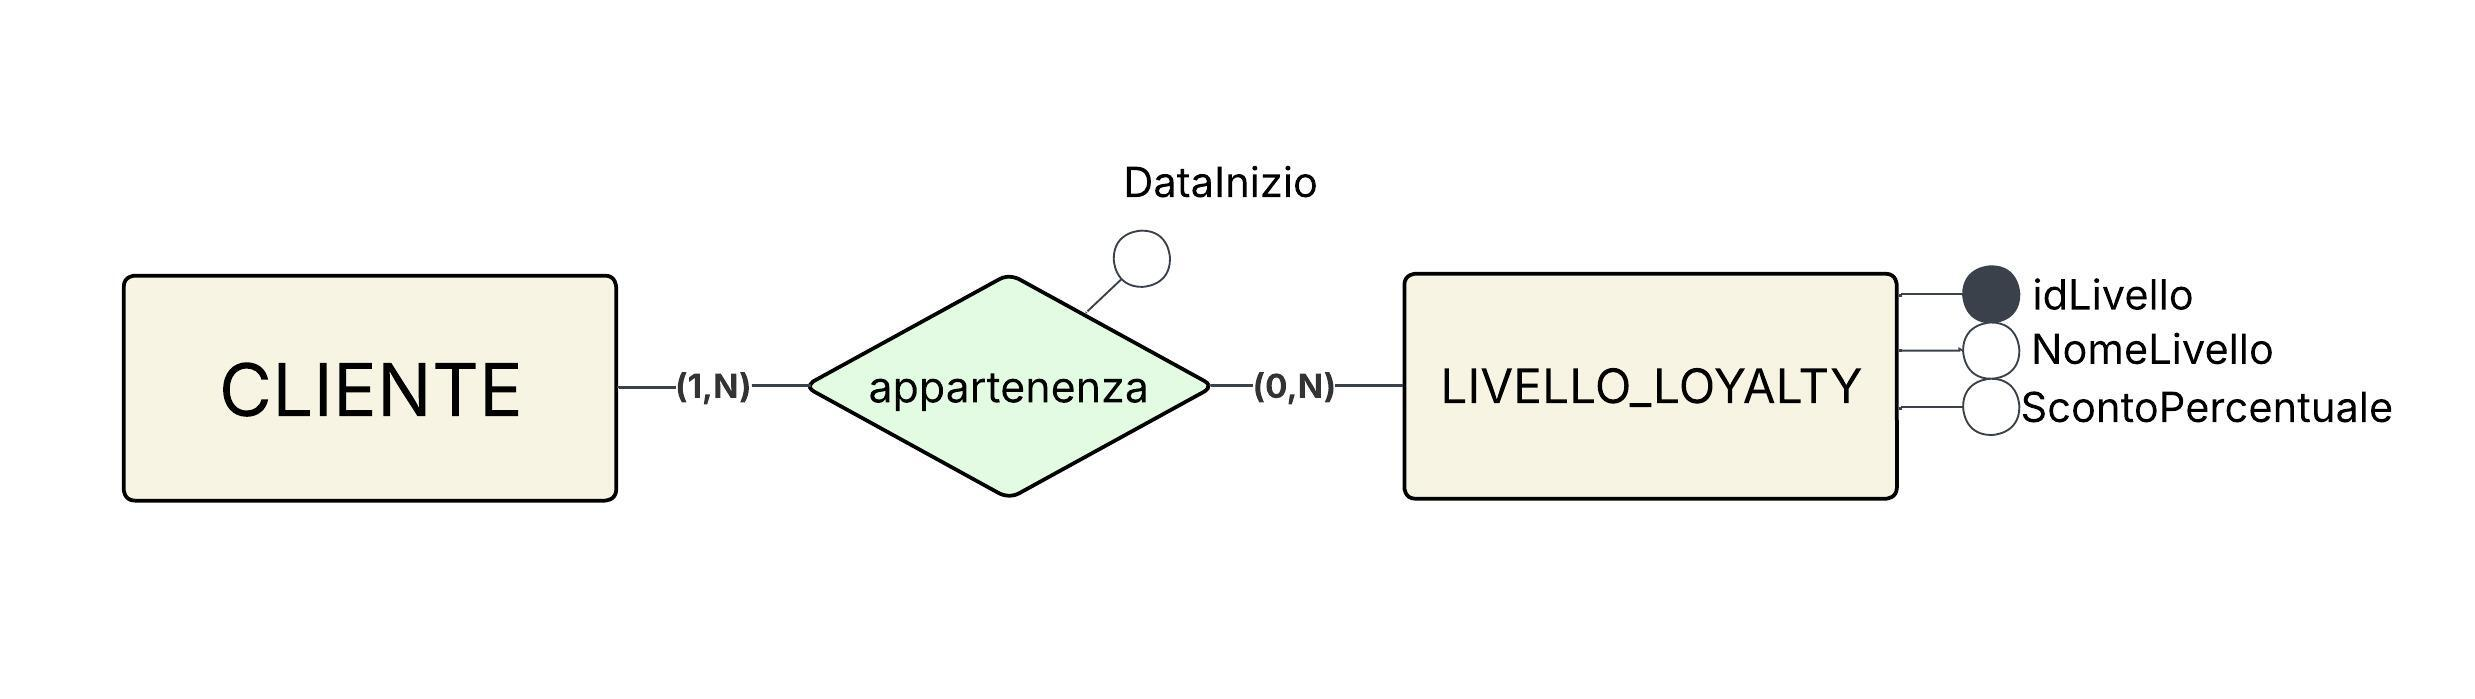
\includegraphics[angle=0,width=\textwidth]{../resources/ER/HotelDB_ER_Cliente-LivelloLoyalty.jpeg}
    \caption{Schema E/R modellazione LIVELLO\_LOYALTY}
\end{figure}

\newpage

\subsection{CONSUMO indipendente da PRENOTAZIONE}
L'associazione \textbf{effettuazione} lega \textbf{CONSUMO} esclusivamente a \textbf{CLIENTE}, e non a \textbf{PRENOTAZIONE}. Un cliente può quindi registrare una o più consumazioni di servizi accessori (ad esempio il noleggio di una bicicletta o l'acquisto di un servizio in area comune) anche senza avere una prenotazione attiva presso l'hotel nel momento in cui il servizio viene erogato.\medskip
\newline
Questa scelta riflette un requisito funzionale esplicito: i servizi accessori dell'hotel non sono riservati esclusivamente agli ospiti con soggiorno in corso, ma possono essere fruiti da qualunque cliente registrato nel sistema, indipendentemente dal proprio stato di prenotazione. Un cliente che ha già effettuato il check-out, o che semplicemente non ha mai prenotato una camera, resta comunque un \textbf{CLIENTE} a tutti gli effetti e può richiedere servizi.\medskip
\newline
Introdurre invece un'associazione diretta tra \textbf{CONSUMO} e \textbf{PRENOTAZIONE} (anche opzionale, con cardinalità (0,1) sul lato prenotazione) avrebbe permesso di risalire immediatamente al soggiorno a cui afferisce una consumazione, ma non è un'informazione richiesta dai requisiti: l'unico vincolo funzionale è che ogni consumazione sia sempre riconducibile a un cliente identificato, non a un soggiorno specifico. Si è quindi scelto di non introdurre questa associazione, in coerenza con il criterio di \textbf{minimalità}: aggiungere un legame che nessun requisito richiede introdurrebbe complessità concettuale non necessaria.

\begin{figure}[H]
    \centering
    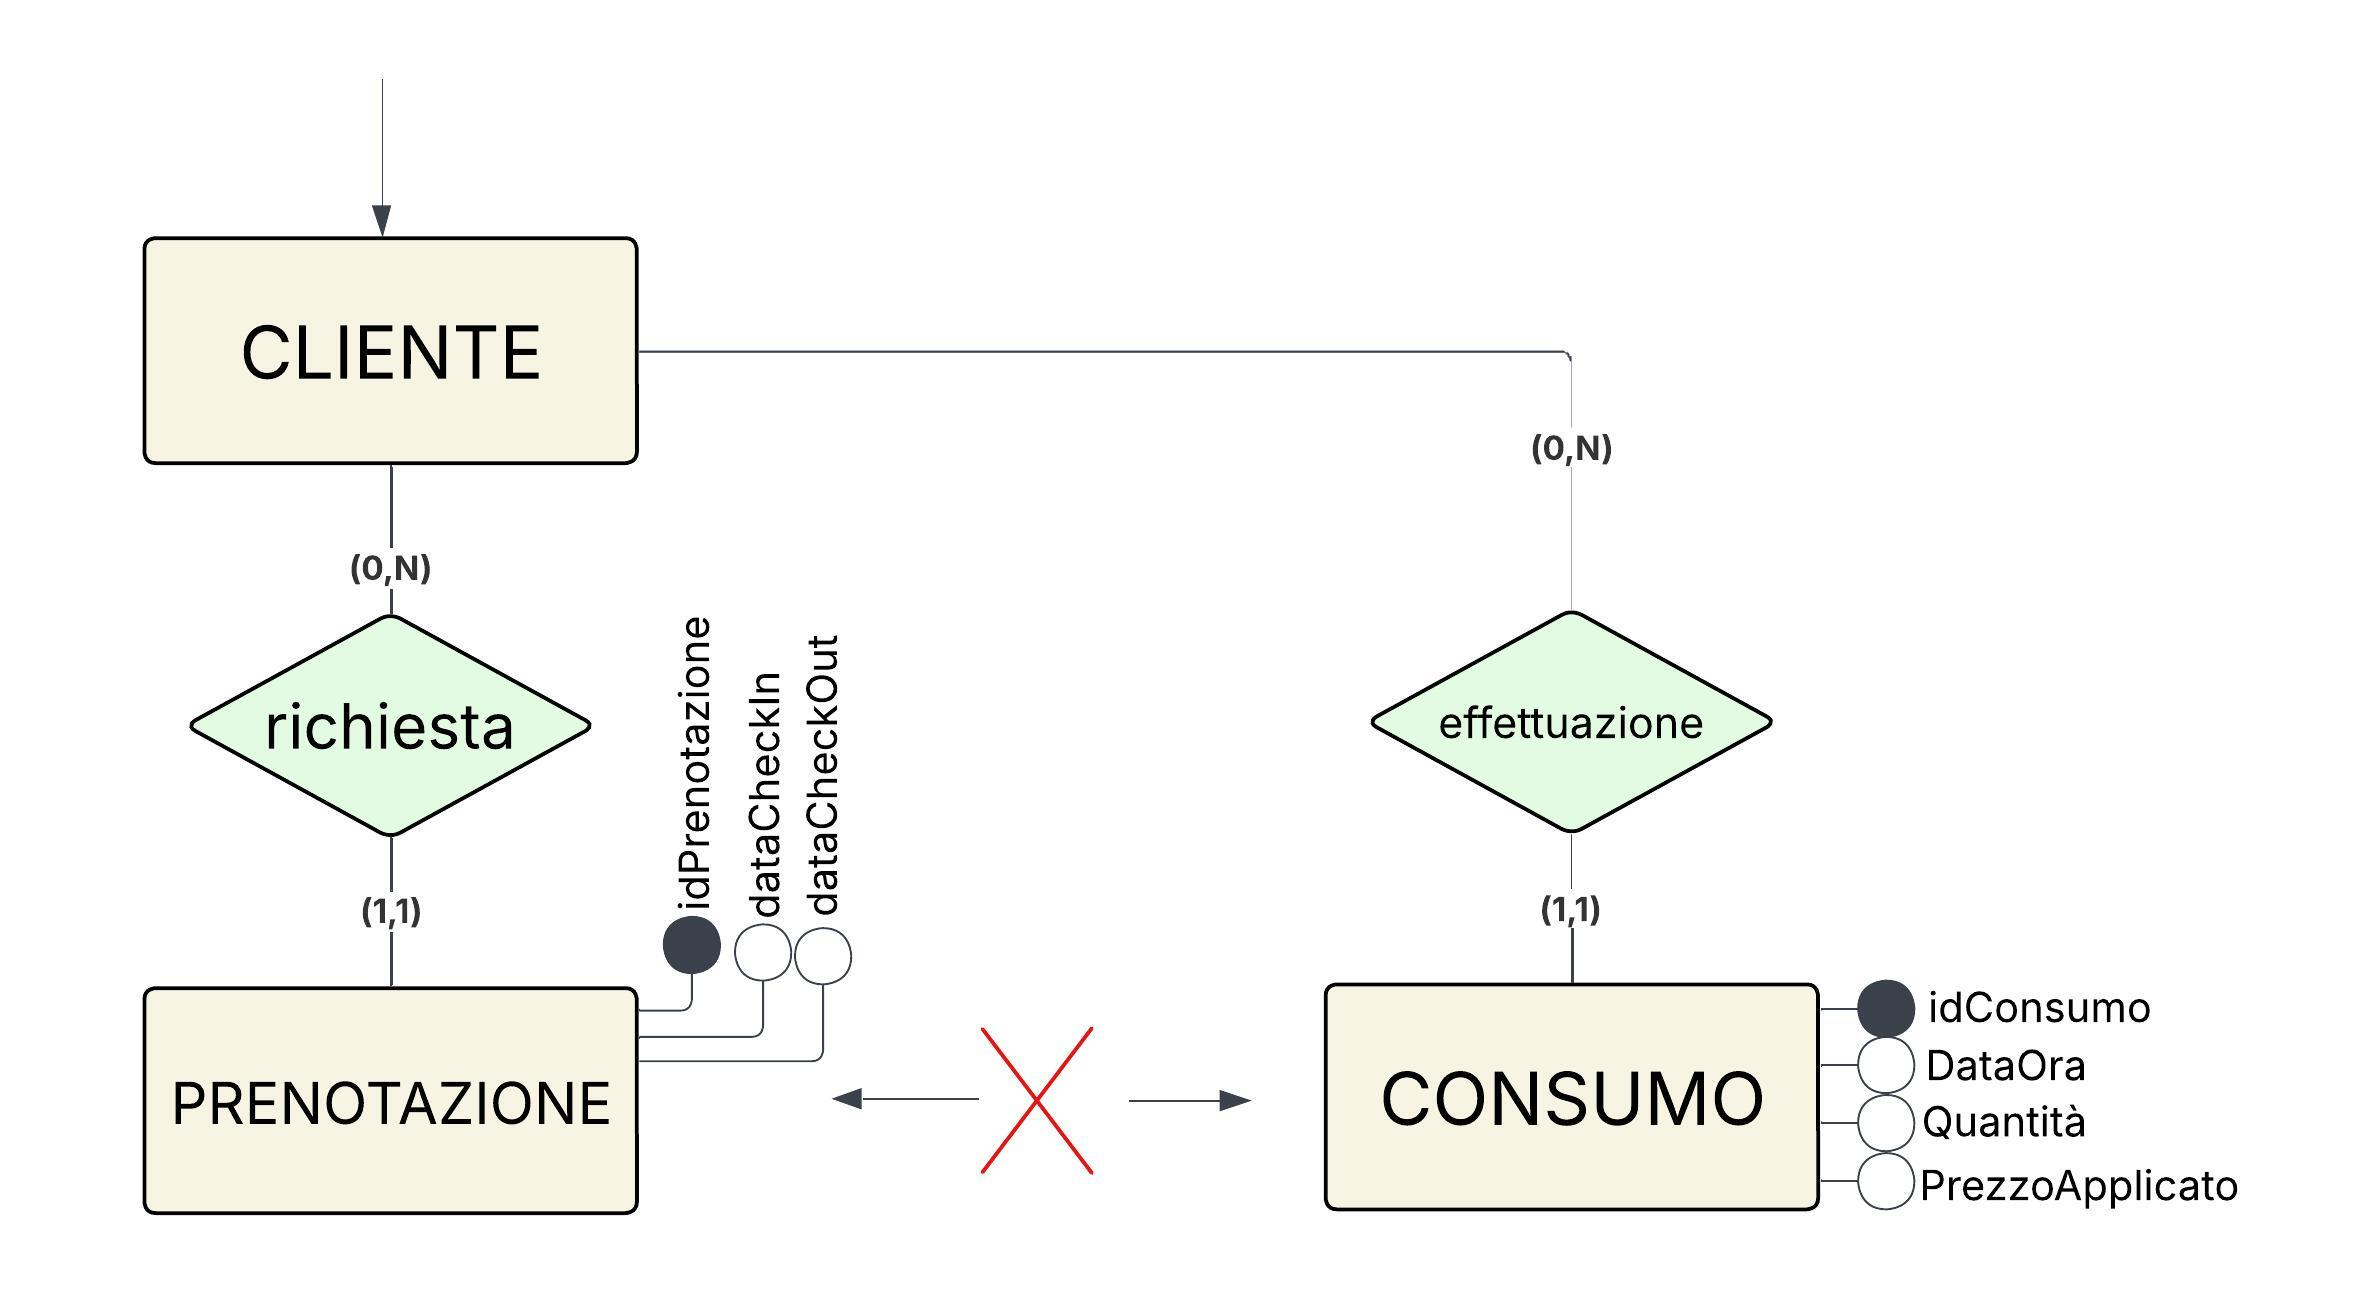
\includegraphics[angle=0,width=0.7\textwidth]{../resources/ER/HotelDB_ER_Consumo-Prenotazione.jpeg}
    \caption{Schema E/R indipendenza Consumo-Prenotazione}
\end{figure}

\newpage

\subsection{CONSUMO e SERVIZIO}
Ogni \textbf{CONSUMO} è relativo a un solo \textbf{SERVIZIO}, mentre uno stesso \textbf{SERVIZIO} può essere oggetto di molte consumazioni nel tempo. L'associazione \textbf{utilizzo} è stata quindi modellata come \textit{uno-a-molti}, con cardinalità (1,1) sul lato \textbf{CONSUMO} e (0,N) sul lato \textbf{SERVIZIO} --- la stessa struttura logica già adottata per l'associazione \textbf{classificazione} tra \textbf{CAMERA} e \textbf{TIPOLOGIA\_CAMERA}.\medskip
\newline
\textbf{SERVIZIO} rappresenta il catalogo statico dei servizi accessori offerti dall'hotel (nome e prezzo unitario correntemente in vigore), mentre \textbf{CONSUMO} rappresenta il singolo evento di utilizzo da parte di un cliente, con i propri attributi \textbf{DataOra}, \textbf{Quantità} e \textbf{PrezzoApplicato}.\medskip
\newline
L'attributo \textbf{PrezzoApplicato} su \textbf{CONSUMO} non è ridondante rispetto a \textbf{PrezzoUnitario} su \textbf{SERVIZIO}, pur essendo concettualmente vicino: rappresenta il prezzo effettivamente applicato al momento della consumazione, che può differire dal prezzo unitario corrente del servizio (ad esempio in caso di promozioni, sconti puntuali, o modifiche del listino avvenute dopo la registrazione della consumazione). Si tratta quindi di un dato storico da preservare indipendentemente da eventuali variazioni successive di \textbf{PrezzoUnitario}, e non di un valore derivabile.

\begin{figure}[H]
    \centering
    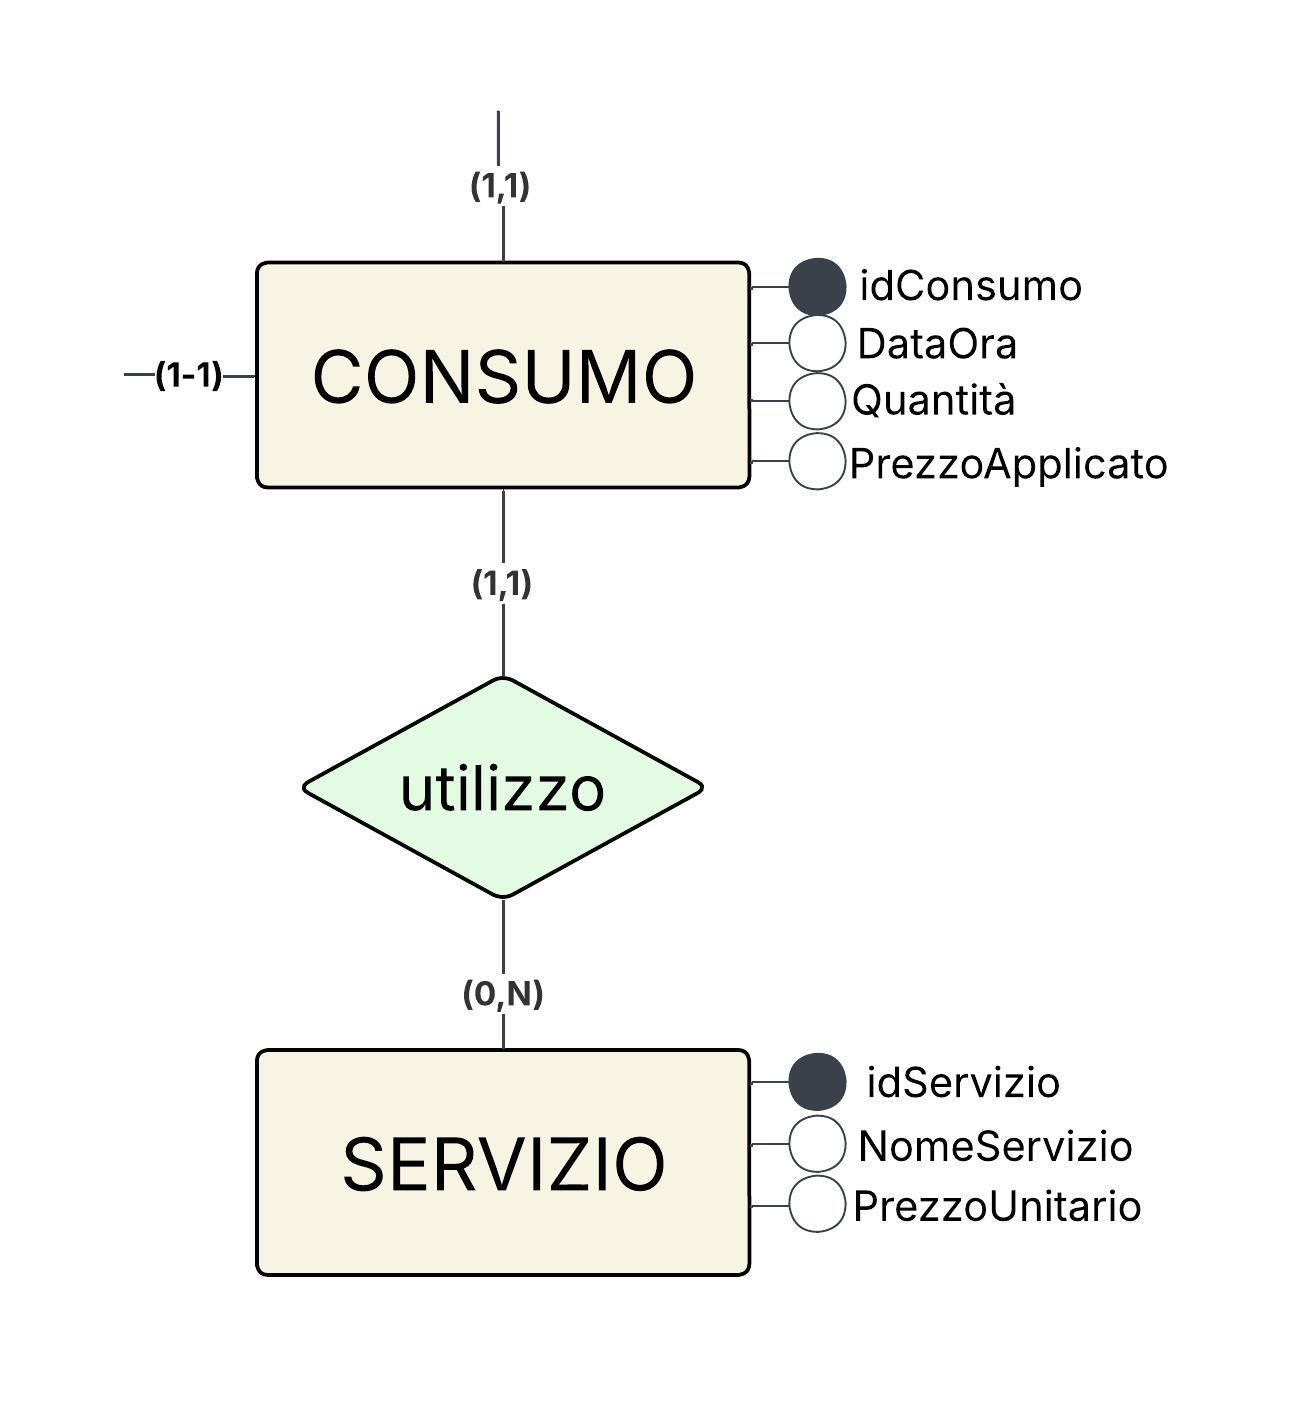
\includegraphics[angle=0,width=0.5\textwidth]{../resources/ER/HotelDB_ER_Consumo-Servizio.jpeg}
    \caption{Schema E/R associazione Consumo-Servizio}
\end{figure}

\newpage

\subsection{Gestione dei Pagamenti}

L'entità \textbf{PAGAMENTO} (\texttt{idPagamento}, \texttt{Importo},
\texttt{DataOra}, \texttt{MetodoPagamento}) rappresenta la registrazione
di un incasso, riferito in modo esclusivo a una \textbf{PRENOTAZIONE}
oppure a una \textbf{CONSUMO}. Sono state introdotte due associazioni
opzionali distinte chiamate \textbf{riferimento} collegate a Prenotazione e Consumo. Entrambe con cardinalità (0,1) - (1,1).
\medskip
\newline
Le due associazioni impongono congiuntamente un vincolo di
\textbf{esclusività reciproca}: ogni \textbf{PAGAMENTO} deve riferirsi a
esattamente una tra \textbf{PRENOTAZIONE} e \textbf{CONSUMO}, mai a
entrambe, mai a nessuna delle due. Questo vincolo, analogamente a quanto
già osservato per la non sovrapposizione temporale delle camere, non è
rappresentabile graficamente mediante le sole cardinalità Chen e viene
quindi gestito tramite controlli applicativi.
\medskip
\newline
Si è scelto un modello di \textbf{pagamento unico e contestuale}: ogni
prenotazione o consumazione ammette al più un pagamento, effettuato nello
stesso momento in cui l'evento viene registrato. Pagamenti parziali,
multipli o differiti nel tempo non sono supportati in questa versione del
progetto ma con possibile estensione
futura non prevista nell'ambito attuale.
\medskip
\newline
L'attributo \textbf{MetodoPagamento} è stato modellato come attributo a
dominio fisso (Carta, Contanti) direttamente su \textbf{PAGAMENTO},
anziché come entità separata: con soli due valori statici, privi di
attributi propri o di necessità di storicizzazione, un'entità dedicata
introdurrebbe complessità concettuale non giustificata da alcun
requisito (a differenza di \textbf{STATO\_PRENOTAZIONE}, che possiede una
reale evoluzione temporale tracciata da \textbf{VARIAZIONE}).
\medskip
\newline
Poiché il pagamento è contestuale alla creazione della prenotazione o
della consumazione, l'operazione ``Registra pagamento'' non viene
modellata come operazione autonoma: è invece incorporata, come
sottopasso automatico, dentro ``Crea prenotazione'' e ``Registra
consumazione servizio'' --- lo stesso trattamento già riservato a
``Calcola sconto Loyalty'' all'interno di ``Crea prenotazione''.

\begin{figure}[H]
    \centering
    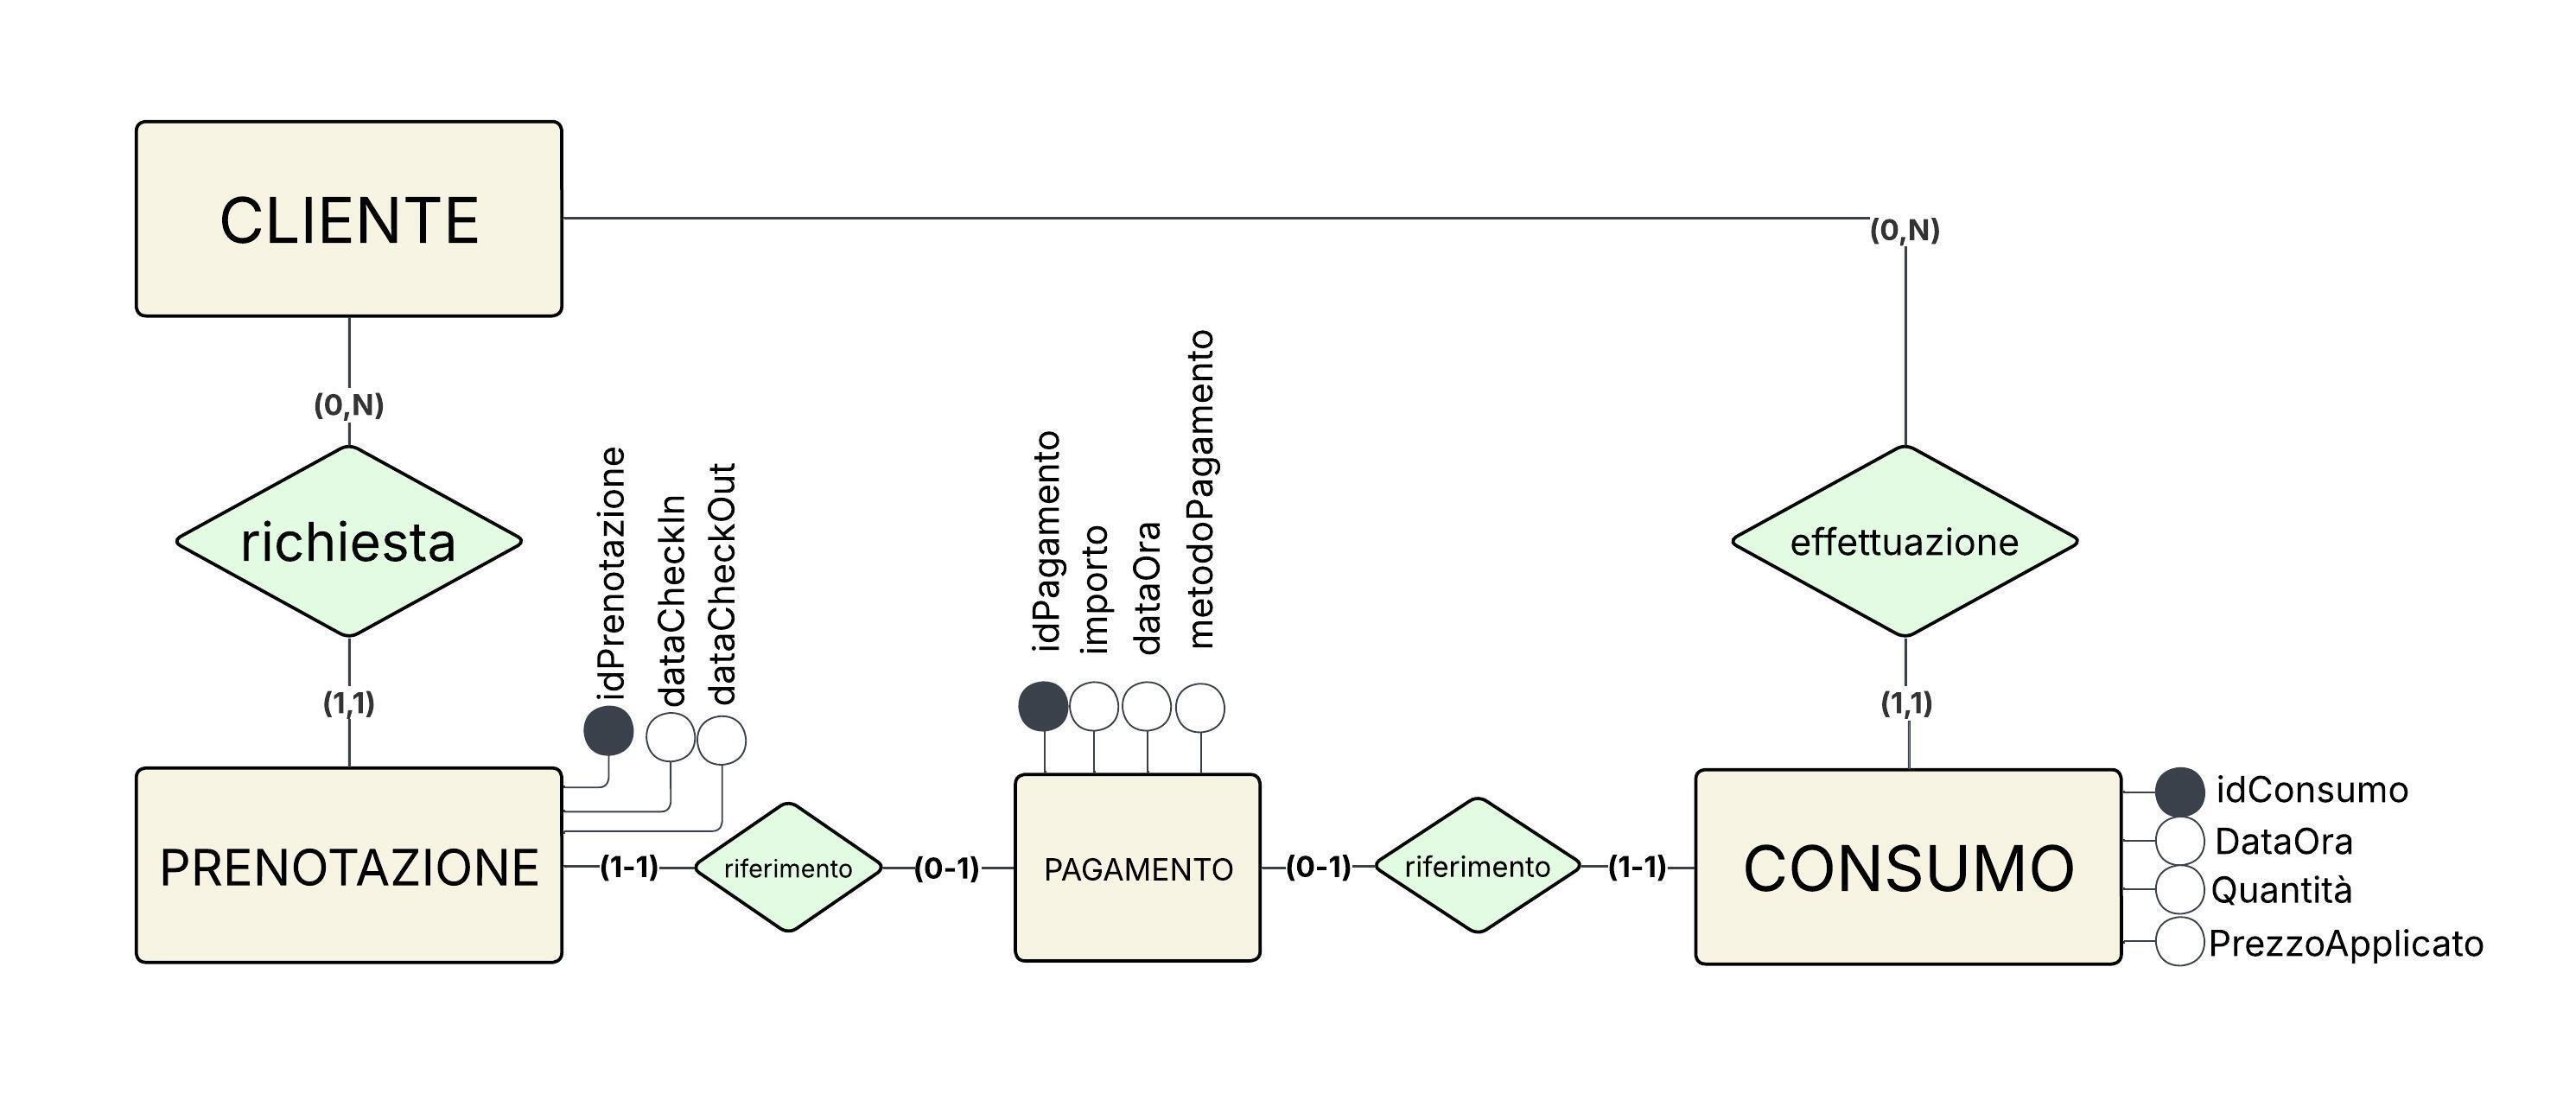
\includegraphics[angle=0,width=\textwidth]{../resources/ER/HotelDB_ER_Pagamento.jpeg}
    \caption{Schema E/R Entità Pagamento}
\end{figure}


\chapter{Progettazione Logica}

\section{Stima del volume dei dati}

Per ogni concetto dello schema concettuale (entità E o associazione A) si stima
il numero di istanze previste, secondo la tavola dei volumi.

\begin{table}[H]
    \centering
    \rowcolors{2}{gray!10}{white}
    \begin{tabular}{|l|c|>{\centering\arraybackslash}p{1.7cm}|p{6.5cm}|}
        \hline
        \rowcolor{headerblue}
        \textbf{Concetto}   & \textbf{Costrutto} & \textbf{Numero Stimato} & \textbf{Motivazione}                                                                                \\
        \hline
        PERSONA             & E                  & 15.000                  & Clienti + personale accumulato nel tempo                                                            \\
        CLIENTE             & E                  & 14.500                  & Clientela storica su più anni                                                                       \\
        UTENTE              & E                  & 18                      & Personale interno                                                                                   \\
        RUOLO               & E                  & 4                       & Admin, Reception, Accounting, Maintenance                                                           \\
        ATTRIBUZIONE        & A                  & 22                      & Coppie Utente-Ruolo; pochi utenti con più di un ruolo                                               \\
        TIPOLOGIA\_CAMERA   & E                  & 8                       & Single, Double Standard, Double Deluxe, Suite...                                                    \\
        CAMERA              & E                  & 80                      & Hotel di medie dimensioni                                                                           \\
        LIVELLO\_LOYALTY    & E                  & 4                       & Bronze, Silver, Gold, Platinum                                                                      \\
        APPARTENENZA        & A                  & 19.000                  & Ogni cliente passa in media per 1-2 livelli nel tempo                                               \\
        PRENOTAZIONE        & E                  & 25.000                  & \textasciitilde{}8.000/anno $\times$ 3 anni                                                         \\
        ASSEGNAZIONE        & A                  & 35.000                  & Alcune prenotazioni includono più camere                                                            \\
        STATO\_PRENOTAZIONE & E                  & 5                       & Requested, Confirmed, Cancelled, CheckedIn, CheckedOut                                              \\
        VARIAZIONE          & A                  & 100.000                 & \textasciitilde{}4 cambi di stato per prenotazione (storico stati)                                  \\
        SERVIZIO            & E                  & 15                      & Colazione, minibar, noleggio biciclette...                                                          \\
        CONSUMO             & E                  & 200.000                 & Più consumi per soggiorno                                                                           \\
        PAGAMENTO           & E                  & 225.000                 & PRENOTAZIONE + CONSUMO (assunzione: quasi ogni prenotazione/consumazione ha un pagamento associato) \\
        \hline
    \end{tabular}
    \caption{Stima dei volumi}
    \label{tab:volumi}
\end{table}

\section{Descrizione delle operazioni principali e stima della loro frequenza}

Per ciascuna operazione principale si specifica il tipo (Interattiva I o
Batch B) e la frequenza media di esecuzione, espressa in numero di
occorrenze al giorno. Le frequenze sono derivate dalla tavola dei volumi
(\cref{tab:volumi}), applicando i rapporti tra i concetti coinvolti,
distribuiti su un arco temporale di riferimento di 3 anni (\textasciitilde{}1.095
giorni), coerentemente con la stima di PRENOTAZIONE.

In accordo con la regola empirica 80-20, l'analisi di dettaglio (schema di
navigazione e tavola degli accessi, \cref{sec:accessi}) verrà svolta per le
operazioni a maggiore frequenza, responsabili della quota preponderante del
carico complessivo sul sistema.

\begin{table}[H]
    \centering
    \rowcolors{2}{gray!10}{white}
    \small
    \makebox[\textwidth][c]{
        \begin{tabular}{|p{5.7cm}|l|c|c|p{4.5cm}|}
            \hline
            \rowcolor{headerblue}
            \textbf{Operazione}                                                                  & \textbf{Attore} & \textbf{Tipo} & \textbf{Freq.}          & \textbf{Motivazione}                               \\
            \hline
            \hyperref[sec:RegistraCliente]{Registra nuovo cliente}                               & Reception       & I             & 8/g                     & Nuovi clienti nel tempo                            \\
            \hyperref[sec:CreaPrenotazione]{Crea prenotazione}                                   & Reception       & I             & 23/g                    & 25.000 / 1.095 giorni                              \\
            \hyperref[sec:AssegnaCamera]{Assegna camera/e a prenotazione}                        & Reception       & I             & 32/g                    & ASSEGNAZIONE / 1.095 giorni                        \\
            \hyperref[sec:CambiaStato]{Cambia stato prenotazione}                                & Reception       & I             & 92/g                    & VARIAZIONE / 1.095 giorni                          \\
            \hyperref[sec:RegistraConsumazione]{Registra consumazione servizio}                  & Reception       & I             & 183/g                   & CONSUMO / 1.095 giorni                             \\
            \hyperref[sec:AssegnaLivello]{Assegna livello loyalty a cliente}                     & Reception       & I             & 17/g                    & APPARTENENZA / 1.095 giorni                        \\
            \hyperref[sec:AggiornaStatoCamera]{Aggiorna stato camera}                            & Maintenance     & I             & 46/g                    & \textasciitilde{}2 per prenotazione (check-in/out) \\
            \hyperref[sec:ConsultaDisponibilita]{Consulta disponibilità camere in un intervallo} & Reception       & I             & 50/g                    & Consultata più volte per prenotazione              \\
            \hyperref[sec:ConsultaPrenotazioniData]{Consulta prenotazioni per data}              & Reception       & I             & 10/g                    & Controllo giornaliero (soggiorno attivo)           \\
            \hyperref[sec:AssegnaRuolo]{Assegna ruolo a utente}                                  & Admin           & I             & 0,07/g (2/mese)         & 22 ATTRIBUZIONE totali                             \\
            \hyperref[sec:TipologiaCameraOp]{Crea/modifica tipologia camera}                     & Admin           & I             & \textasciitilde{}0,03/g & Configurazione quasi statica (stima simbolica)     \\
            \hyperref[sec:ServizioOp]{Crea/modifica servizio accessorio}                         & Admin           & I             & \textasciitilde{}0,03/g & Configurazione quasi statica (stima simbolica)     \\
            \hyperref[sec:FatturatoGiornaliero]{Calcola fatturato giornaliero}                   & Accounting      & B             & 1/g                     & Aggregazione notturna automatica                   \\
            \hyperref[sec:IncassiGiornalieri]{Calcola incassi giornalieri}                       & Accounting      & B             & 1/g                     & Aggregazione notturna automatica                   \\
            \hline
        \end{tabular}
    }
    \caption{Operazioni principali e stima della frequenza}
    \label{tab:operazioni}
\end{table}

\section{Schemi di navigazione e tabelle degli accessi}
\label{sec:accessi}

In questa sezione si costruiscono, per \emph{tutte} le operazioni principali
individuate in \cref{tab:operazioni}, lo schema di navigazione e la
relativa tavola degli accessi.
\newline
Convenzioni adottate in tutta la sezione:
\begin{itemize}
    \item il costo degli accessi in scrittura è considerato doppio
          rispetto a quello delle letture: costo pesato per esecuzione $= L + 2S$;
    \item tutte le frequenze sono espresse in accessi/giorno, per
          permettere il confronto diretto nella tavola di sintesi finale;
    \item quando il numero di istanze coinvolte non è semplicemente presente nella tavola dei volumi (\cref{tab:volumi}), l'assunzione
          statistica adottata è dichiarata esplicitamente nel paragrafo di
          analisi che ne fa uso.
\end{itemize}

\subsection{Registra nuovo cliente}
\label{sec:RegistraCliente}

Operazione di inserzione: crea una nuova istanza di \textbf{PERSONA} e la
corrispondente istanza di \textbf{CLIENTE} lungo la generalizzazione
parziale sovrapposta descritta in Progettazione Concettuale. Poiché la
cardinalità (1,N) sul lato \textbf{CLIENTE} dell'associazione
\textbf{appartenenza} impone che ogni cliente possieda sempre almeno un
livello loyalty, la creazione di un nuovo cliente comporta automaticamente
l'inserimento di una riga in \textbf{APPARTENENZA} con il livello loyalty
base (es. ``Bronze'') e \texttt{DataInizio} pari alla data di
registrazione.

\begin{figure}[H]
    \centering
    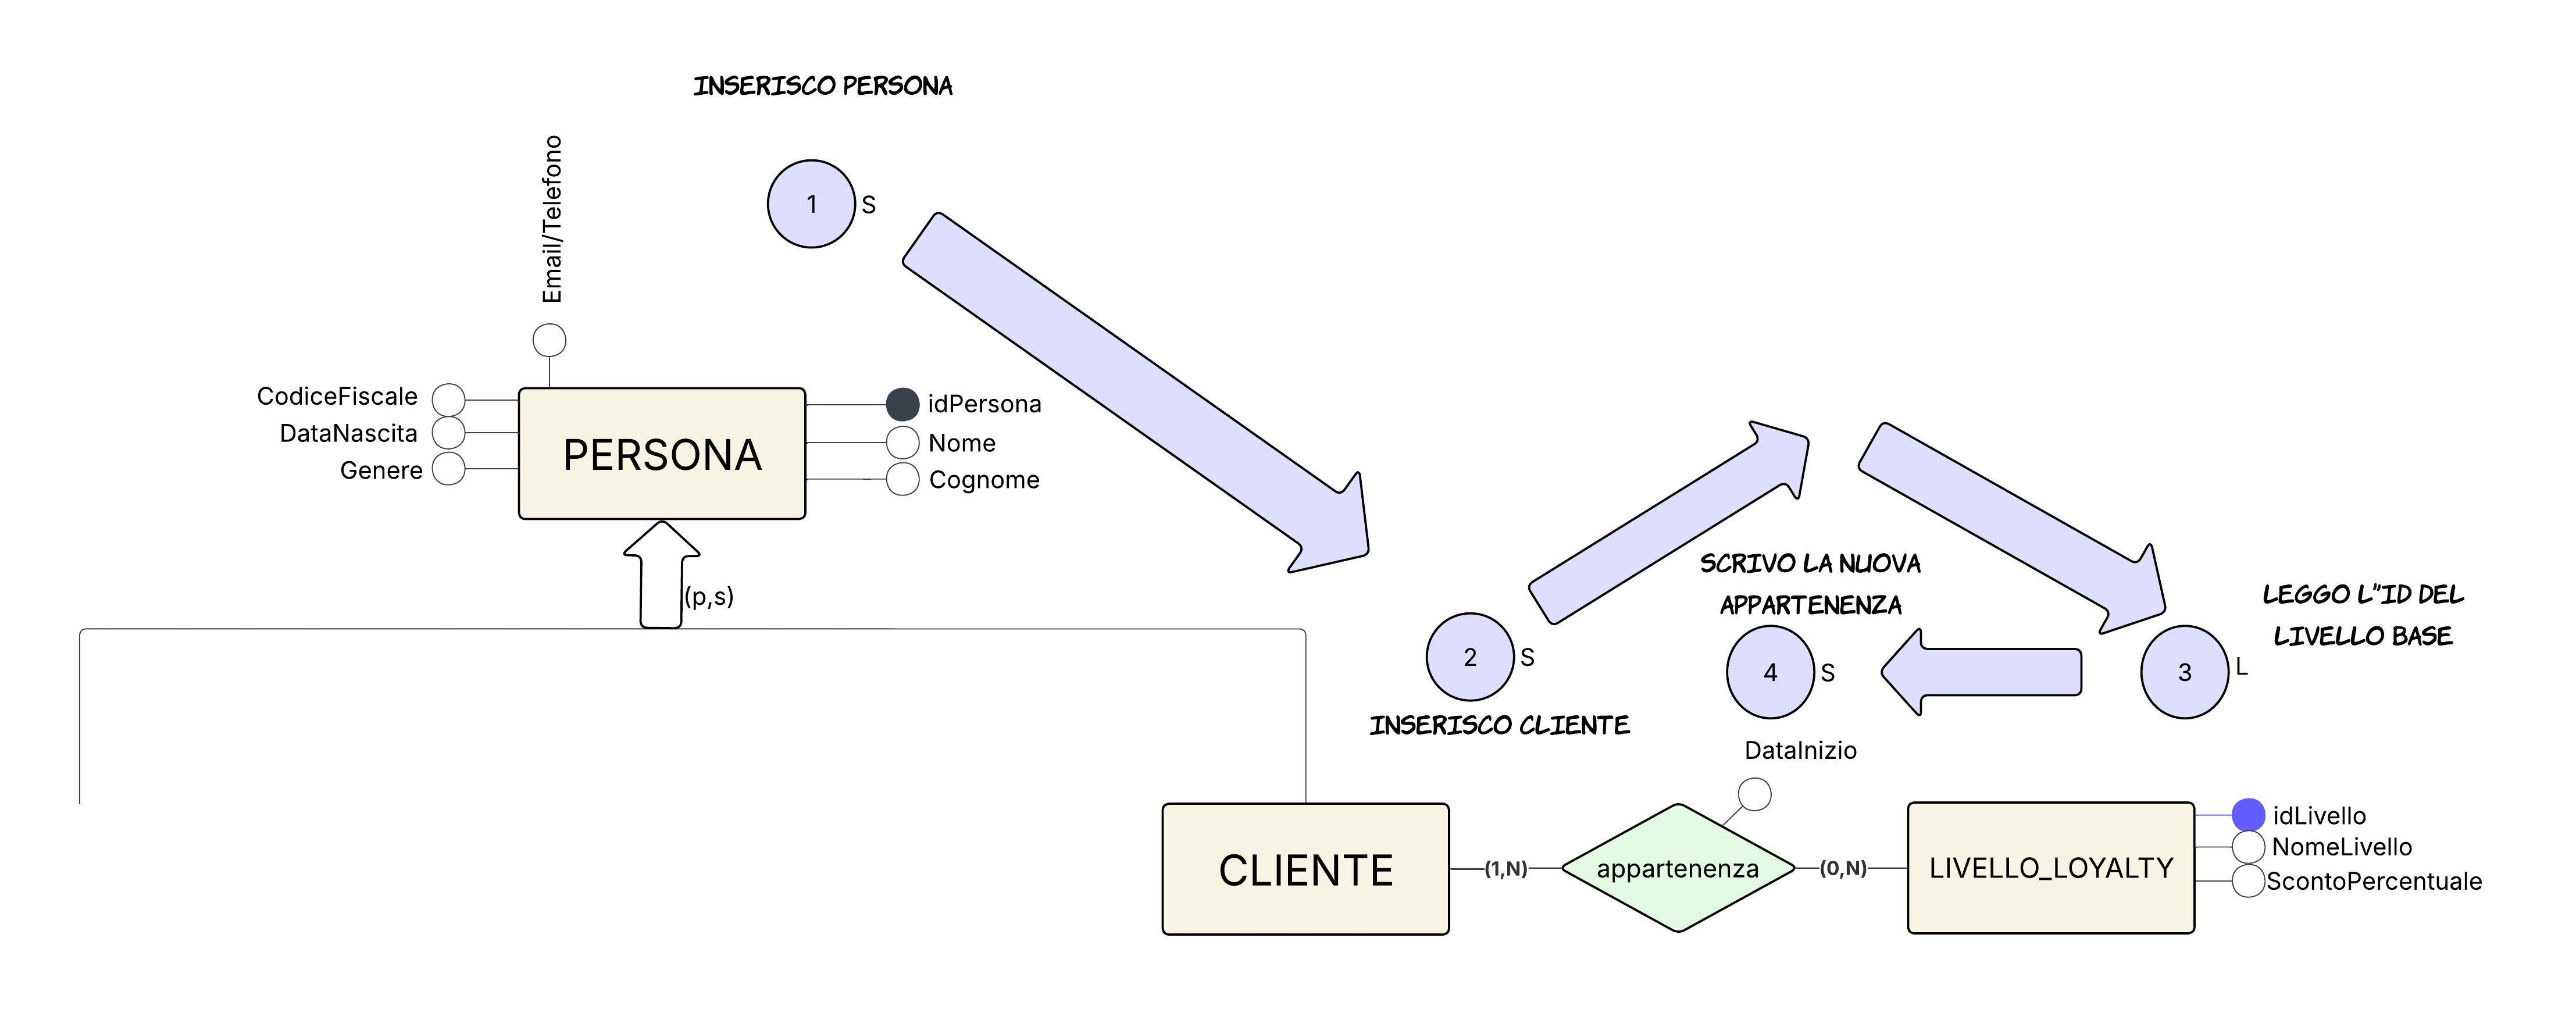
\includegraphics[width=\textwidth]{../resources/nav/HotelDB_Nav_RegistraCliente.jpeg}
    \caption{Schema di navigazione --- Registra nuovo cliente}
\end{figure}

\begin{table}[H]
    \centering
    \rowcolors{2}{gray!10}{white}
    \begin{tabular}{|l|c|c|c|}
        \hline
        \rowcolor{headerblue}
        \textbf{Concetto} & \textbf{Costrutto} & \textbf{Accessi} & \textbf{Tipo}    \\
        \hline
        PERSONA           & E                  & 1                & S                \\
        CLIENTE           & E                  & 1                & S                \\
        LIVELLO\_LOYALTY  & E                  & 1                & L                \\
        APPARTENENZA      & A                  & 1                & S                \\
        \hline
        \rowcolor{gray!25}
        \textbf{Totale}   &                    & \textbf{4}       & \textbf{1L + 3S} \\
        \hline
    \end{tabular}
    \caption{Tavola degli accessi --- Registra nuovo cliente}
\end{table}

Costo giornaliero dell'operazione $= (1L + 3S{\times}2) \times 8 = 56$
accessi/giorno.

\subsection{Crea prenotazione}
\label{sec:CreaPrenotazione}

L'operazione crea una \textbf{PRENOTAZIONE} per un \textbf{CLIENTE}
esistente e, come già detto nella fase concettuale, inserisce
automaticamente una riga in \textbf{VARIAZIONE} con stato ``Requested'':
per questo motivo l'operazione tocca anche \textbf{STATO\_PRENOTAZIONE}
(per recuperare l'id dello stato ``Requested") pur non
modificandolo. La lettura di \textbf{APPARTENENZA}/\textbf{LIVELLO\_LOYALTY}
serve a determinare lo sconto loyalty da applicare.
\medskip
\newline
\underline{Calcola sconto Loyalty} è un'operazione automatica del Sistema, eseguita una volta per ogni \textit{Crea prenotazione} (stessa frequenza, 23/g):
\smallskip
\newline
Dato un cliente, risale tramite \textbf{APPARTENENZA} al \textbf{LIVELLO\_LOYALTY} correntemente posseduto per leggerne \texttt{ScontoPercentuale}. Individuare la riga ``corrente'' di \textbf{APPARTENENZA} richiede una interrogazione sullo storico ordinato per \texttt{DataInizio}.
La \texttt{DataInizio} più recente è quella attribuita al livello attuale
\smallskip
\newline
Si stima un numero medio di righe coinvolte pari al rapporto ${APPARTENENZA}/{CLIENTE} = 19.000/14.500 \approx 1{,}3$.

\begin{figure}[H]
    \centering
    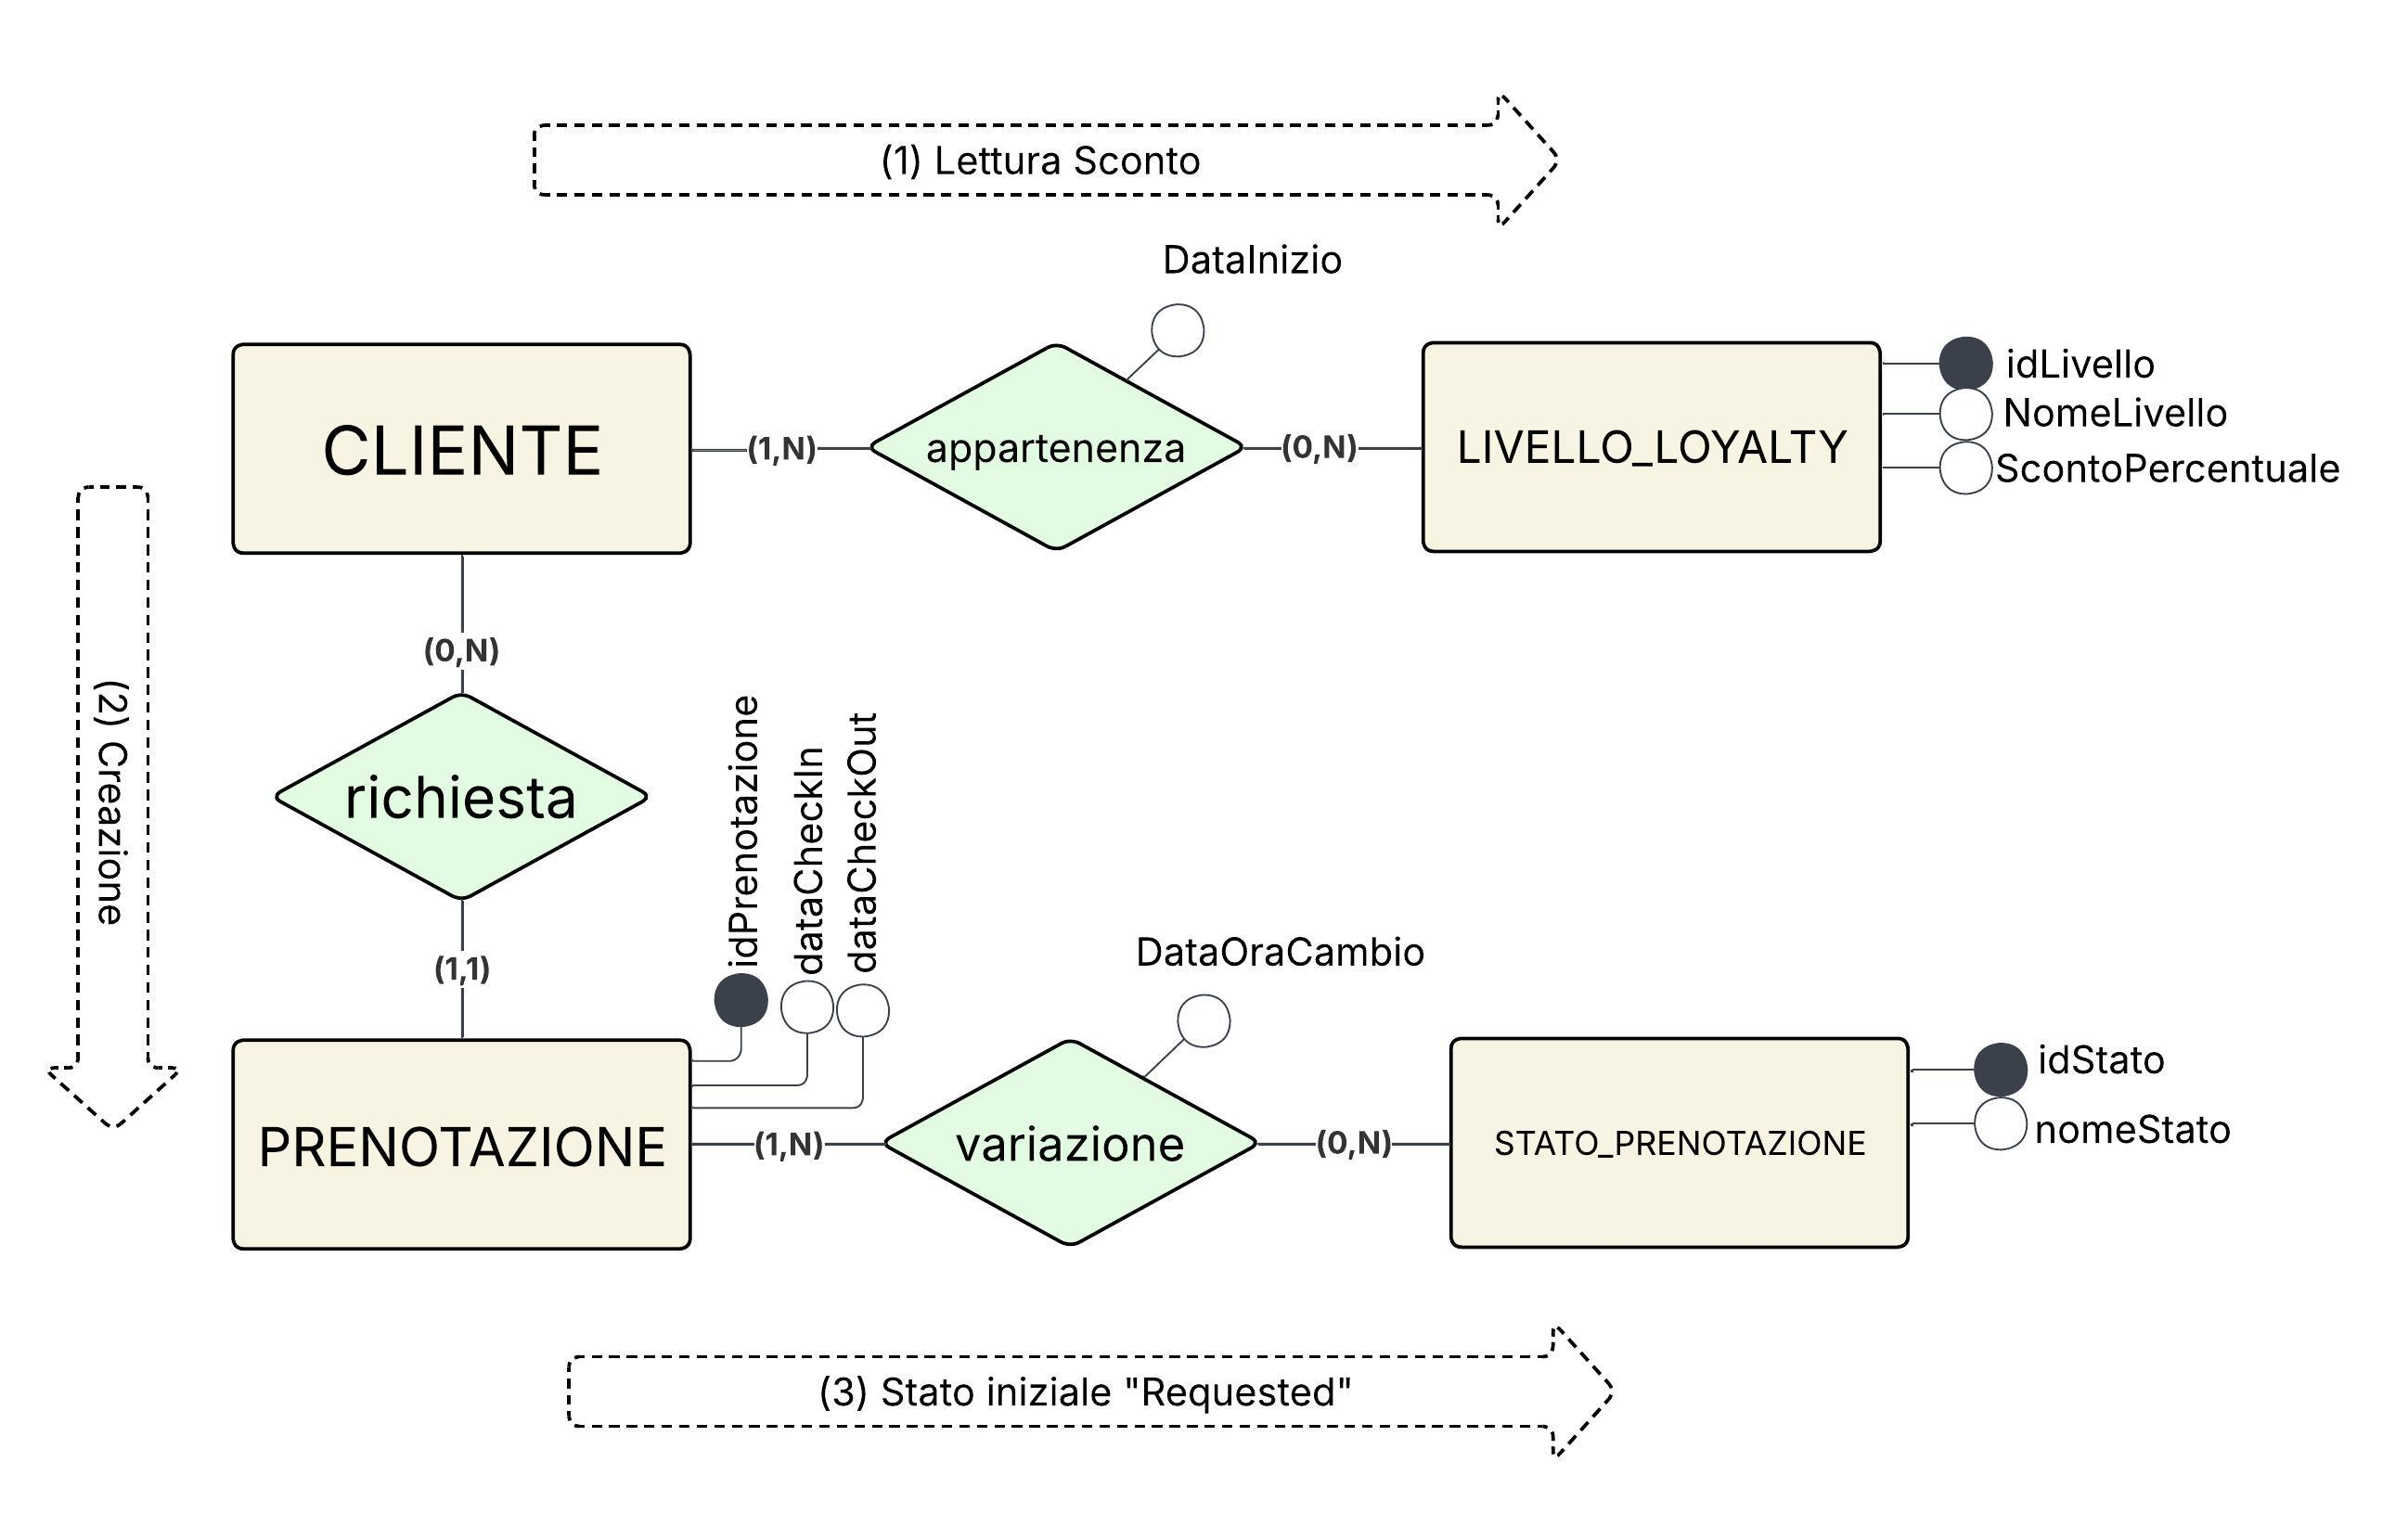
\includegraphics[width=0.60\textwidth]{../resources/nav/HotelDB_Nav_CreaPrenotazione.jpeg}
    \caption{Schema di navigazione --- Crea prenotazione}
\end{figure}

\begin{table}[H]
    \centering
    \rowcolors{2}{gray!10}{white}
    \begin{tabular}{|l|c|c|c|}
        \hline
        \rowcolor{headerblue}
        \textbf{Concetto}   & \textbf{Costrutto} & \textbf{Accessi} & \textbf{Tipo}      \\
        \hline
        CLIENTE             & E                  & 1                & L                  \\
        APPARTENENZA        & A                  & 1,3              & L                  \\
        LIVELLO\_LOYALTY    & E                  & 1                & L                  \\
        PRENOTAZIONE        & E                  & 1                & S                  \\
        STATO\_PRENOTAZIONE & E                  & 1                & L                  \\
        VARIAZIONE          & A                  & 1                & S                  \\
        PAGAMENTO           & E                  & 1                & S                  \\
        \hline
        \rowcolor{gray!25}
        \textbf{Totale}     &                    & \textbf{7,3}     & \textbf{4,3L + 3S} \\
        \hline
    \end{tabular}
    \caption{Tavola degli accessi --- Crea prenotazione}
\end{table}

Costo giornaliero dell'operazione $= (4,3L + 3S{\times}2) \times 23 = 236,9 \approx 237$ accessi/giorno.

\subsection{Assegna camera/e a prenotazione}
\label{sec:AssegnaCamera}

Associa una o più camere disponibili a una prenotazione già creata,
scrivendo altrettante righe in \textbf{ASSEGNAZIONE}. Il numero medio di
camere per prenotazione si stima dal rapporto
${ASSEGNAZIONE}/{PRENOTAZIONE} = 35.000/25.000 = 1{,}4$.

\begin{figure}[H]
    \centering
    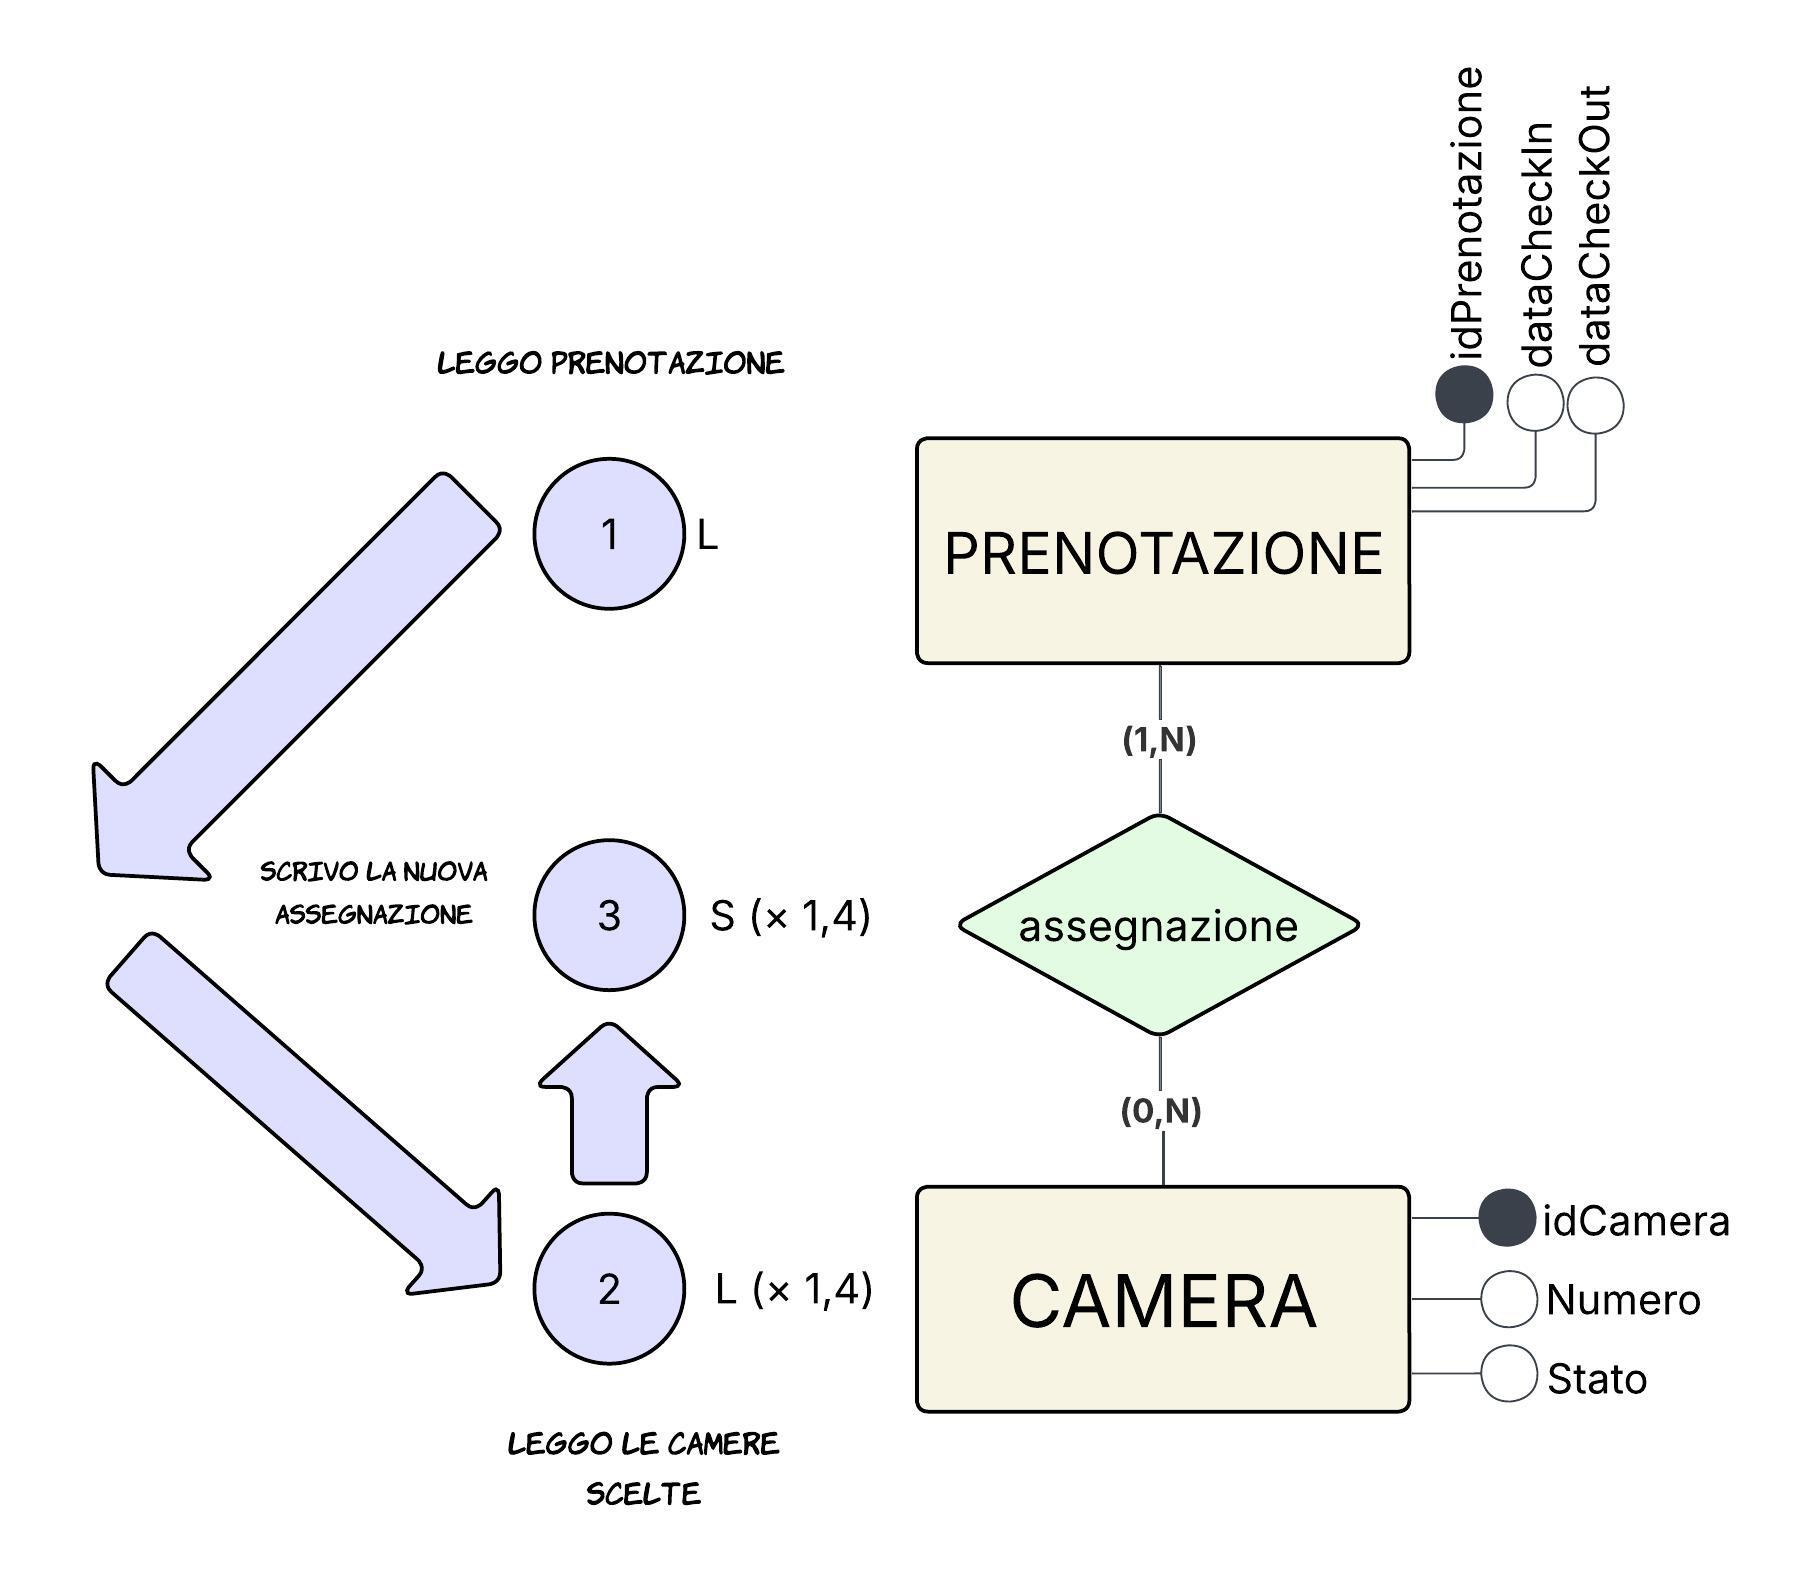
\includegraphics[width=0.55\textwidth]{../resources/nav/HotelDB_Nav_AssegnaCamera.jpeg}
    \caption{Schema di navigazione --- Assegna camera/e a prenotazione}
\end{figure}

\begin{table}[H]
    \centering
    \rowcolors{2}{gray!10}{white}
    \begin{tabular}{|l|c|c|c|}
        \hline
        \rowcolor{headerblue}
        \textbf{Concetto} & \textbf{Costrutto} & \textbf{Accessi}              & \textbf{Tipo}        \\
        \hline
        PRENOTAZIONE      & E                  & 1                             & L                    \\
        CAMERA            & E                  & 1,4                           & L                    \\
        ASSEGNAZIONE      & A                  & 1,4                           & S                    \\
        \hline
        \rowcolor{gray!25}
        \textbf{Totale}   &                    & \textbf{\textasciitilde{}3,8} & \textbf{2.4L + 1.4S} \\
        \hline
    \end{tabular}
    \caption{Tavola degli accessi --- Assegna camera/e a prenotazione}
\end{table}

Costo giornaliero dell'operazione $= (2{,}4L + 1{,}4S{\times}2) \times 32
    \approx 166$ accessi/giorno.

\subsection{Cambia stato prenotazione}
\label{sec:CambiaStato}

Inserisce una nuova riga in \textbf{VARIAZIONE} per registrare un cambio
di stato (es. Confirmed, CheckedIn). L'operazione non deve leggere lo storico
precedente per determinare lo stato corrente: si limita ad aggiungere la
nuova riga, il che la rende economica nonostante sia, in frequenza, la
seconda operazione più eseguita del sistema (92/g).
\newline
Anche se lo \texttt{STATO} viene aggiornato in \textit{CheckOut}, non va comunque fatta una scrittura su prenotazione per aggiornare \textit{dataCheckOut} dato che è una informazione statica fornita nel momento in cui si crea la prenotazione.

\begin{figure}[H]
    \centering
    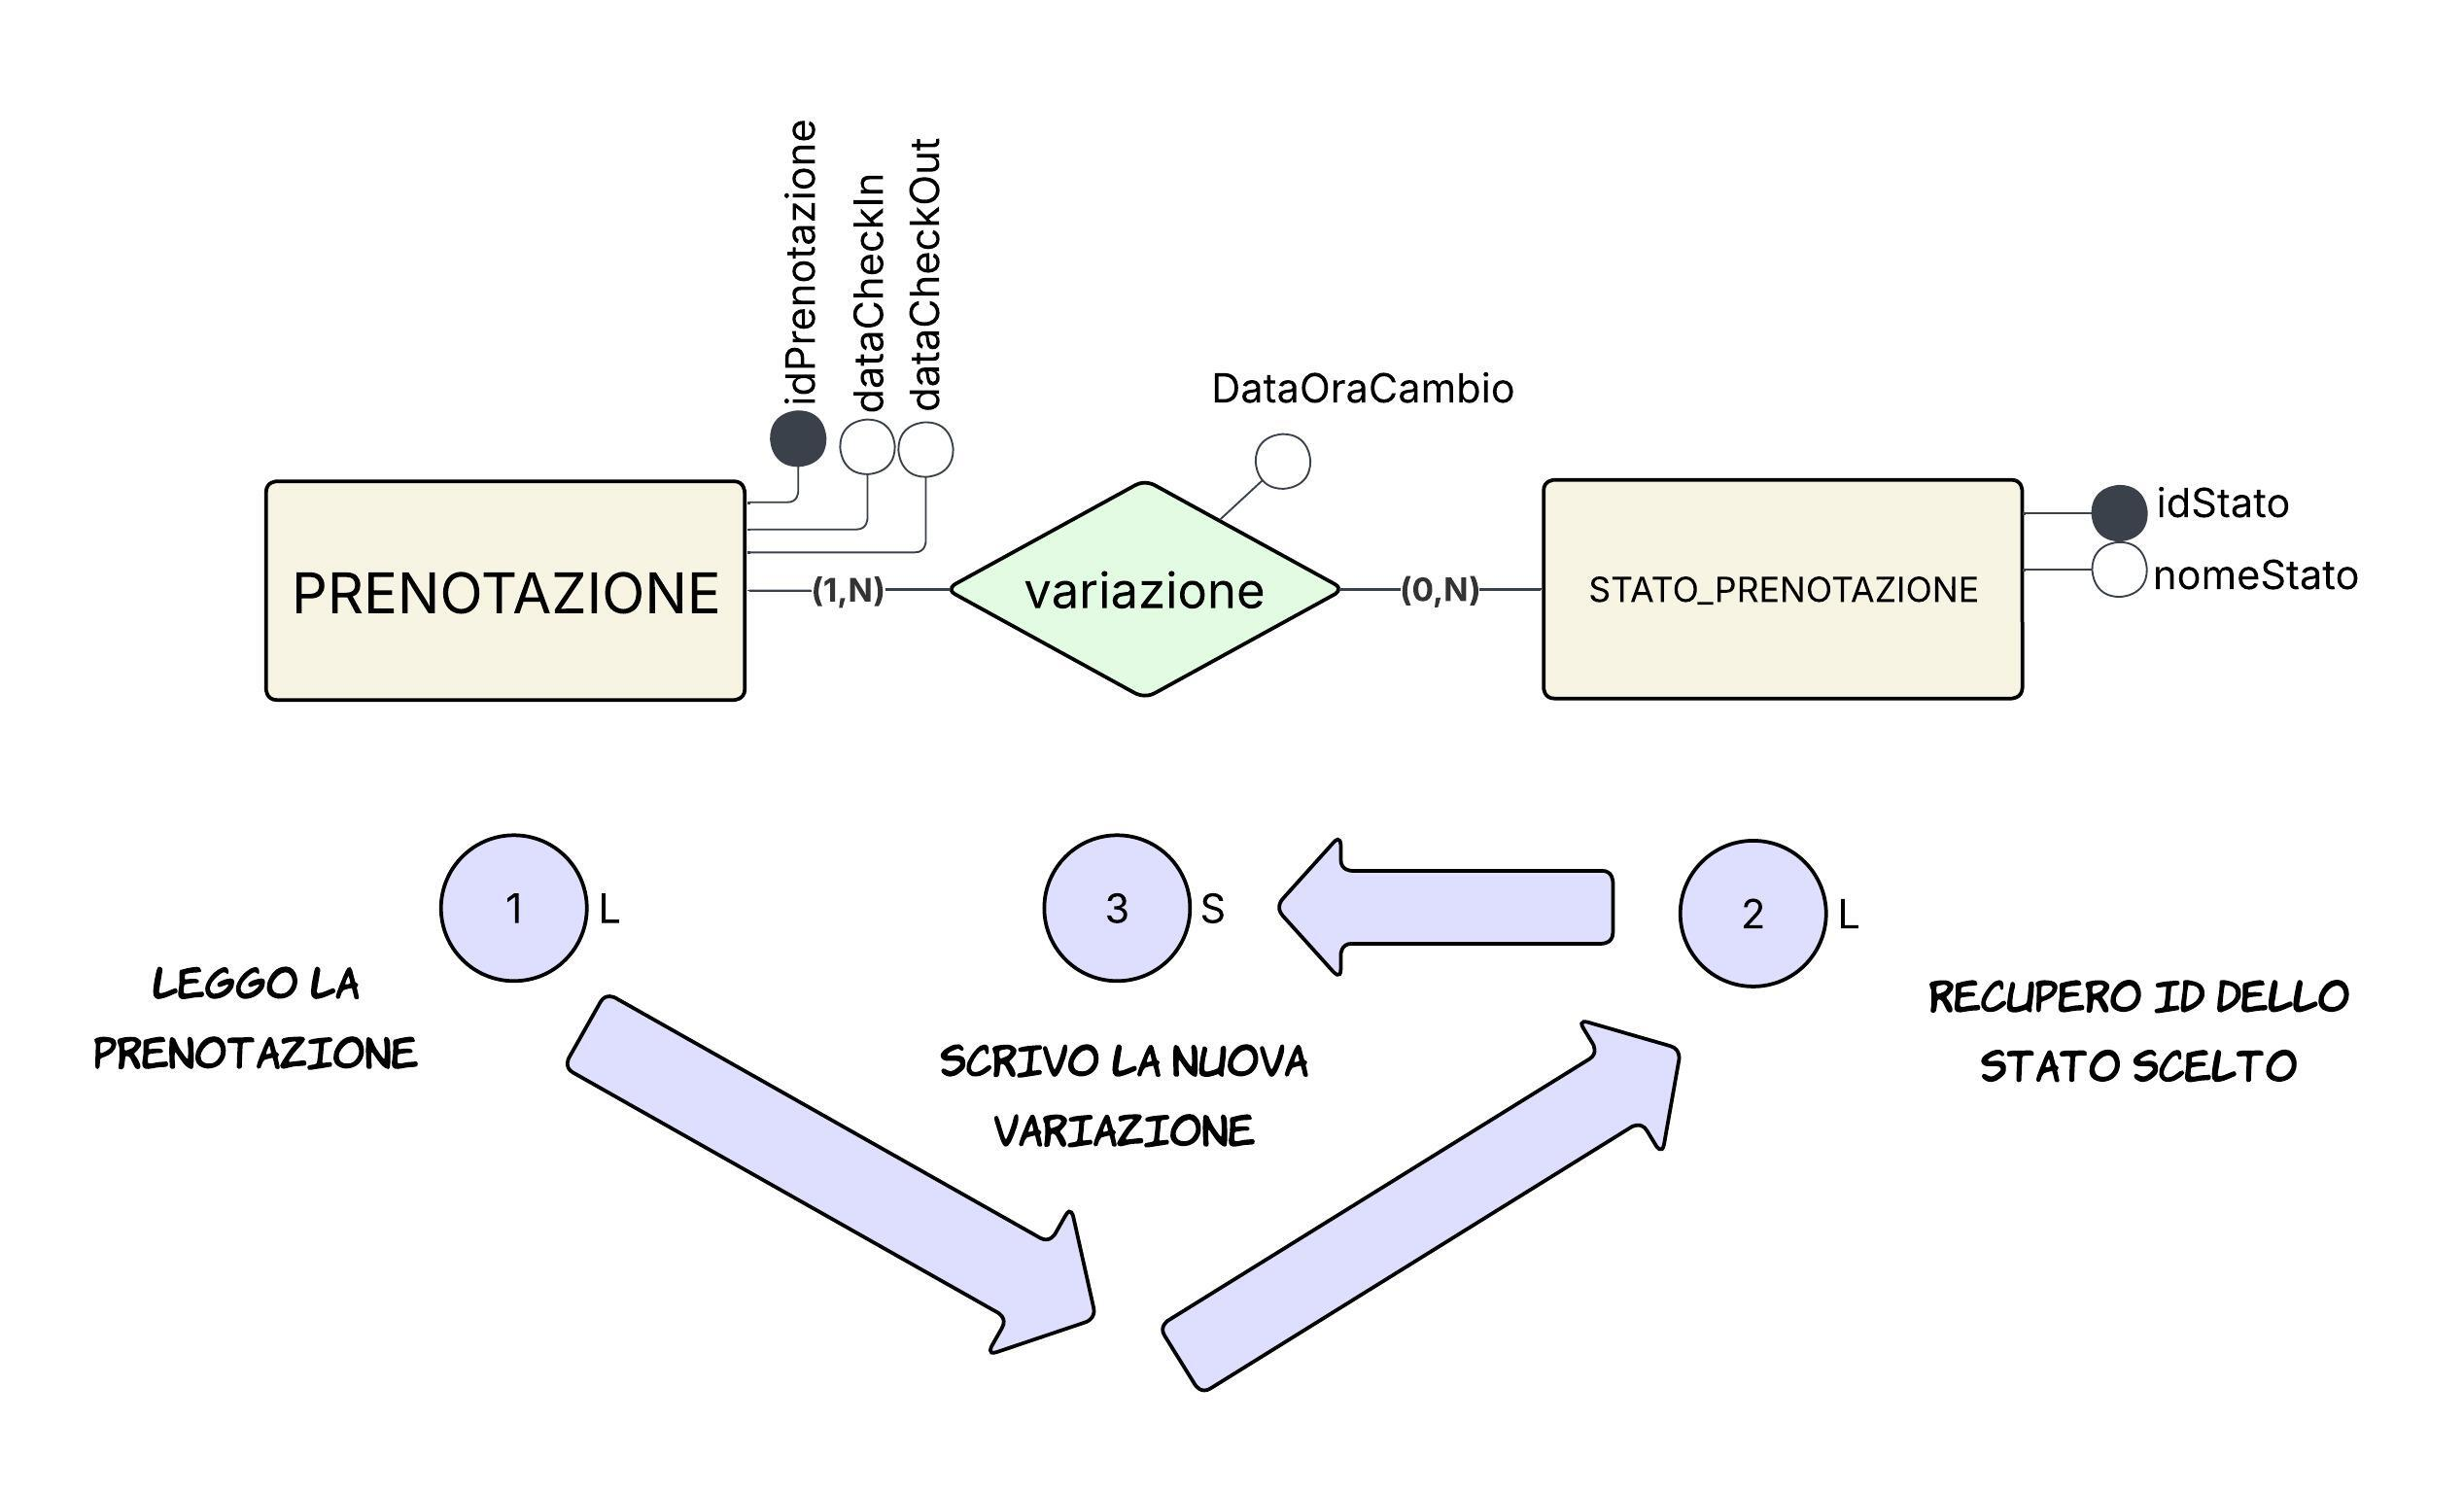
\includegraphics[width=0.55\textwidth]{../resources/nav/HotelDB_Nav_CambiaStato.jpeg}
    \caption{Schema di navigazione --- Cambia stato prenotazione}
\end{figure}

\begin{table}[H]
    \centering
    \rowcolors{2}{gray!10}{white}
    \begin{tabular}{|l|c|c|c|}
        \hline
        \rowcolor{headerblue}
        \textbf{Concetto}   & \textbf{Costrutto} & \textbf{Accessi} & \textbf{Tipo}    \\
        \hline
        PRENOTAZIONE        & E                  & 1                & L                \\
        STATO\_PRENOTAZIONE & E                  & 1                & L                \\
        VARIAZIONE          & A                  & 1                & S                \\
        \hline
        \rowcolor{gray!25}
        \textbf{Totale}     &                    & \textbf{3}       & \textbf{2L + 1S} \\
        \hline
    \end{tabular}
    \caption{Tavola degli accessi --- Cambia stato prenotazione}
\end{table}

Costo giornaliero dell'operazione $= (2L + 1S{\times}2) \times 92 = 368$
accessi/giorno.

\subsection{Registra consumazione servizio}
\label{sec:RegistraConsumazione}

L'operazione collega \textbf{CLIENTE} a \textbf{SERVIZIO} passando per
\textbf{CONSUMO}. Trattandosi di un'associazione binaria semplice
(\textbf{CONSUMO} è legato solo a \textbf{CLIENTE}, mai a
\textbf{PRENOTAZIONE}, come da decisione concettuale), il cammino logico è
lineare. Nonostante sia l'operazione più frequente del sistema (183/g), il
costo per esecuzione resta basso: buon esempio di come alta frequenza non
implichi necessariamente alto costo unitario — a differenza del carico
\emph{complessivo}, che invece resta comunque significativo proprio a
causa della frequenza (si veda \cref{sec:sintesiCarico}).

\begin{figure}[H]
    \centering
    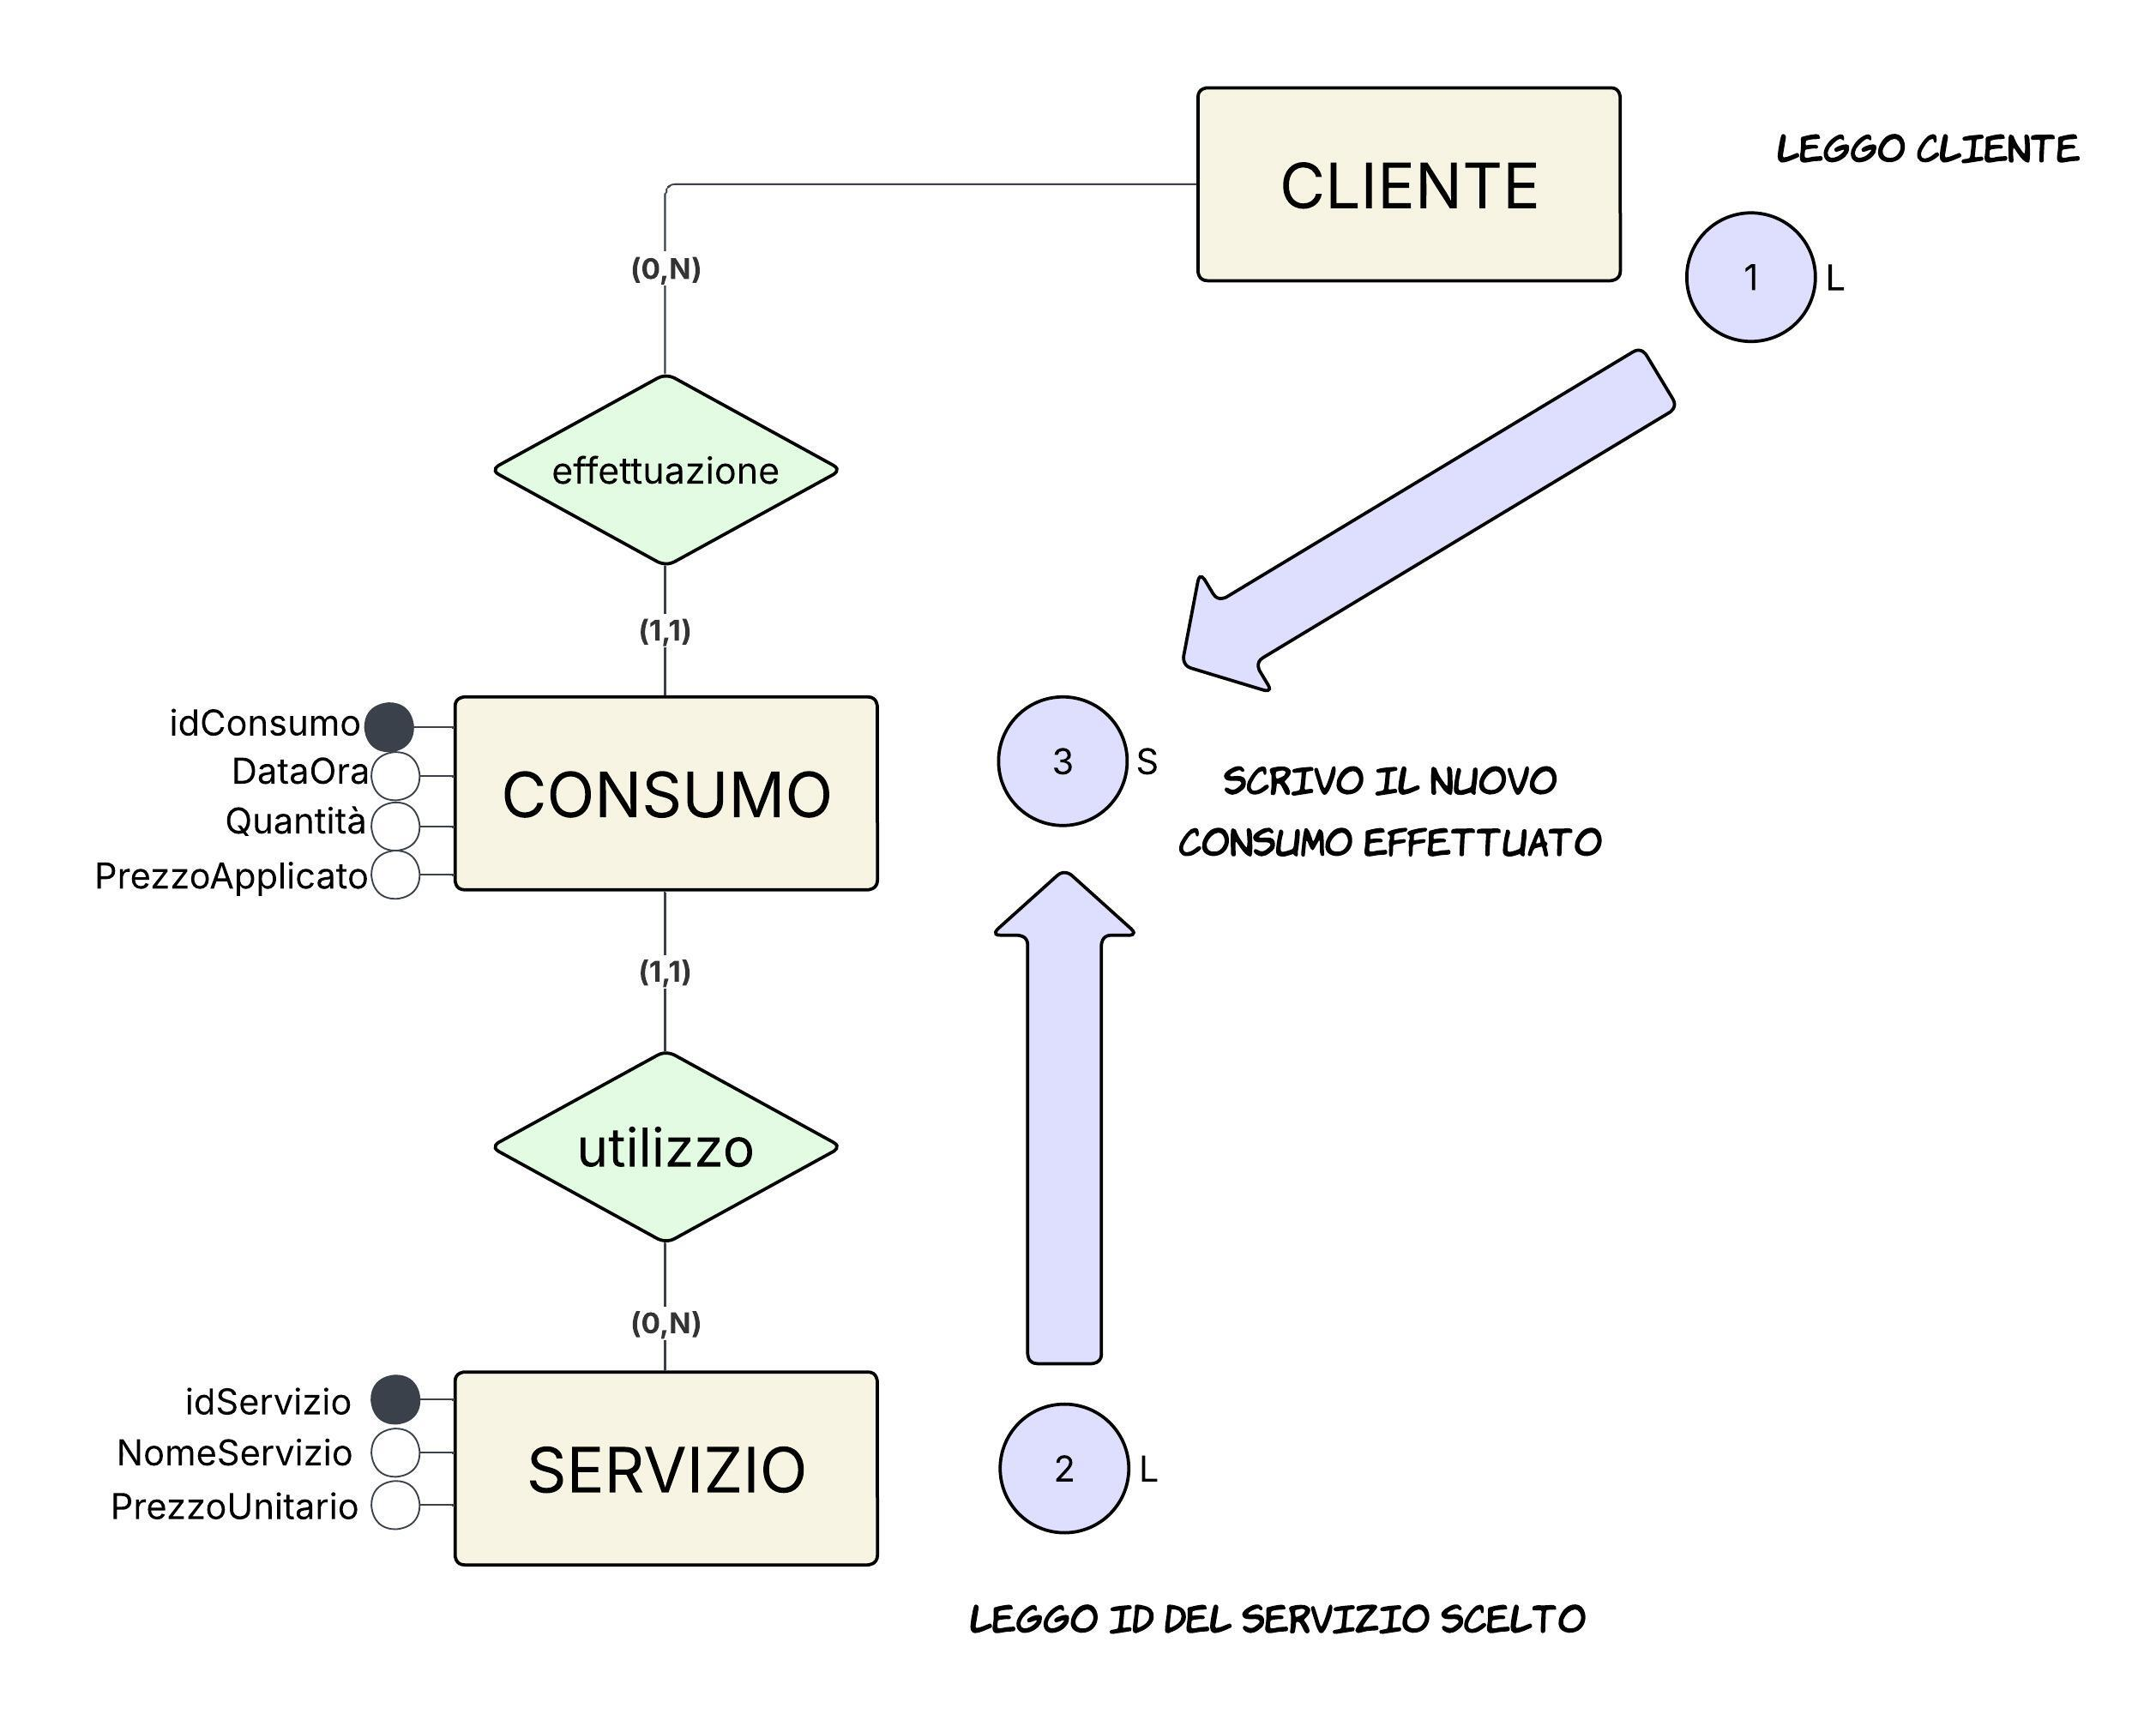
\includegraphics[width=0.55\textwidth]{../resources/nav/HotelDB_Nav_RegistraConsumazione.jpeg}
    \caption{Schema di navigazione --- Registra consumazione servizio}
\end{figure}

\begin{table}[H]
    \centering
    \rowcolors{2}{gray!10}{white}
    \begin{tabular}{|l|c|c|c|}
        \hline
        \rowcolor{headerblue}
        \textbf{Concetto} & \textbf{Costrutto} & \textbf{Accessi} & \textbf{Tipo}    \\
        \hline
        CLIENTE           & E                  & 1                & L                \\
        SERVIZIO          & E                  & 1                & L                \\
        CONSUMO           & E                  & 1                & S                \\
        PAGAMENTO         & E                  & 1                & S                \\
        \hline
        \rowcolor{gray!25}
        \textbf{Totale}   &                    & \textbf{4}       & \textbf{2L + 2S} \\
        \hline
    \end{tabular}
    \caption{Tavola degli accessi --- Registra consumazione servizio}
\end{table}

Costo giornaliero dell'operazione $= (2L + 2S{\times}2) \times 183 = 1098$
accessi/giorno.

\subsection{Assegna livello loyalty a cliente}
\label{sec:AssegnaLivello}

Inserisce una nuova riga in \textbf{APPARTENENZA} con la
\texttt{DataInizio} del nuovo livello. Stessa struttura di
\textit{Cambia stato prenotazione}: nessuna lettura dello storico
precedente è necessaria per la scrittura, perché la decisione di non
introdurre \texttt{DataFine} (presa in fase concettuale) rende
l'operazione di scrittura indipendente dalle righe già presenti --- il
costo di quella scelta di minimalità si paga solo in lettura, nelle
operazioni che devono \emph{ricostruire} il livello corrente, non qui.

\begin{figure}[H]
    \centering
    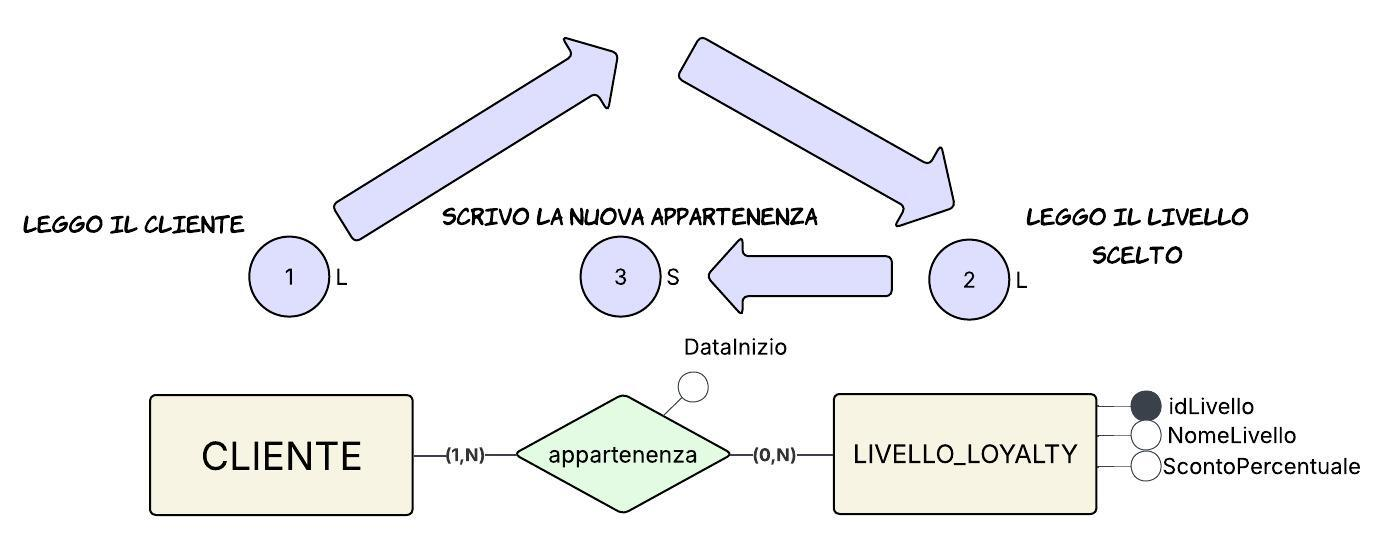
\includegraphics[width=0.55\textwidth]{../resources/nav/HotelDB_Nav_AssegnaLivelloLoyalty.jpeg}
    \caption{Schema di navigazione --- Assegna livello loyalty a cliente}
\end{figure}

\begin{table}[H]
    \centering
    \rowcolors{2}{gray!10}{white}
    \begin{tabular}{|l|c|c|c|}
        \hline
        \rowcolor{headerblue}
        \textbf{Concetto} & \textbf{Costrutto} & \textbf{Accessi} & \textbf{Tipo}    \\
        \hline
        CLIENTE           & E                  & 1                & L                \\
        LIVELLO\_LOYALTY  & E                  & 1                & L                \\
        APPARTENENZA      & A                  & 1                & S                \\
        \hline
        \rowcolor{gray!25}
        \textbf{Totale}   &                    & \textbf{3}       & \textbf{2L + 1S} \\
        \hline
    \end{tabular}
    \caption{Tavola degli accessi --- Assegna livello loyalty a cliente}
\end{table}

Costo giornaliero dell'operazione $= (2L + 1S{\times}2) \times 17 = 68$
accessi/giorno.

\subsection{Aggiorna stato camera}
\label{sec:AggiornaStatoCamera}

Localizza una \textbf{CAMERA} tramite il suo identificativo e ne
aggiorna l'attributo \texttt{Stato}. Nessuna associazione coinvolta: è,
insieme a \textit{Registra nuovo cliente}, l'operazione strutturalmente
più semplice della tavola --- utile a titolo di confronto con
\textit{Registra consumazione servizio}: anche qui, frequenza
alta (46/g, $\sim$2 per prenotazione per check-in/out) ma costo unitario
minimo.

\begin{figure}[H]
    \centering
    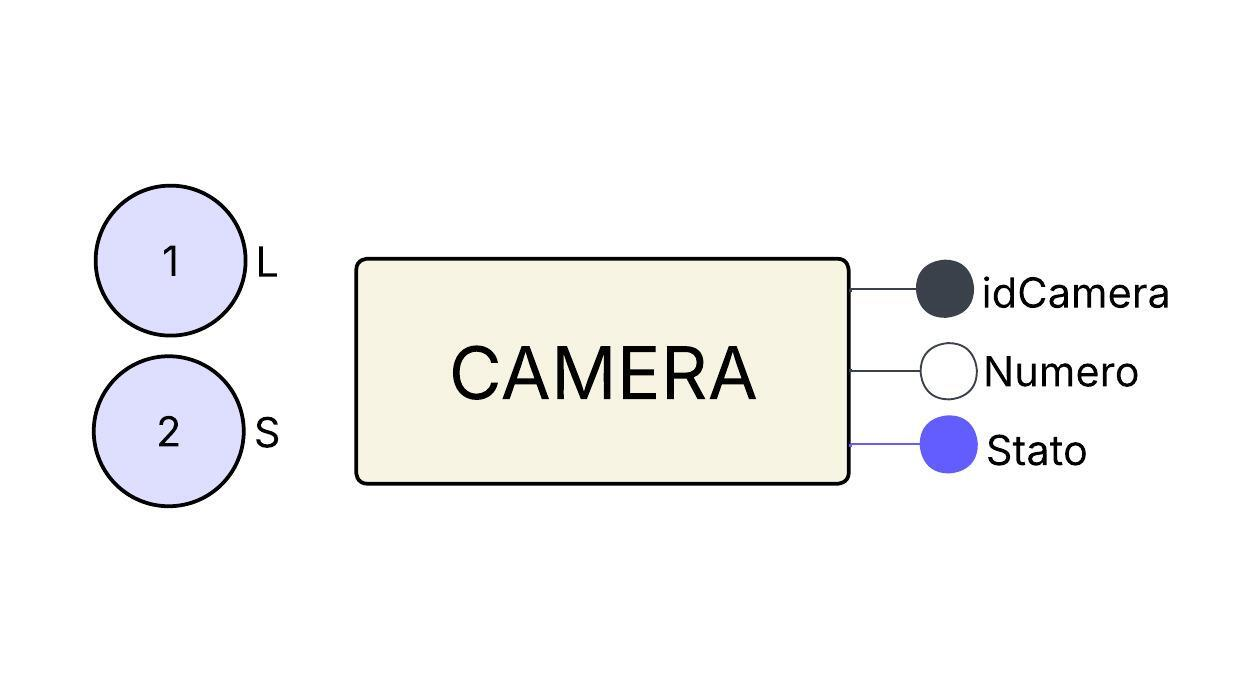
\includegraphics[width=0.40\textwidth]{../resources/nav/HotelDB_Nav_AggiornaStatoCamera.jpeg}
    \caption{Schema di navigazione --- Aggiorna stato camera}
\end{figure}

\begin{table}[H]
    \centering
    \rowcolors{2}{gray!10}{white}
    \begin{tabular}{|l|c|c|c|}
        \hline
        \rowcolor{headerblue}
        \textbf{Concetto} & \textbf{Costrutto} & \textbf{Accessi} & \textbf{Tipo}    \\
        \hline
        CAMERA            & E                  & 1                & L                \\
        CAMERA            & E                  & 1                & S                \\
        \hline
        \rowcolor{gray!25}
        \textbf{Totale}   &                    & \textbf{2}       & \textbf{1L + 1S} \\
        \hline
    \end{tabular}
    \caption{Tavola degli accessi --- Aggiorna stato camera}
\end{table}

Costo giornaliero dell'operazione $= (1L + 1S{\times}2) \times 46 = 138$
accessi/giorno.

\subsection{Consulta disponibilità camere in un intervallo}
\label{sec:ConsultaDisponibilita}

\subsubsection*{Analisi: criteri di ricerca disponibilità}
La ricerca di camere disponibili può avvenire secondo due criteri, non
alternativi: per \textbf{tipologia specifica} (filtro su
\texttt{NomeTipologia}) o per \textbf{capacità} (filtro solo su
\texttt{NumeroLetti} di \textbf{TIPOLOGIA\_CAMERA}, indipendentemente
dalla tipologia). Entrambi sono coperti dagli attributi già presenti in
\textbf{TIPOLOGIA\_CAMERA}. Ai fini della tavola degli accessi si
considera il caso più oneroso --- ricerca per capacità, che nel caso
peggiore coinvolge tutte le 80 camere anziché il sottoinsieme di una
singola tipologia (in media $80/8=10$ camere).

L'operazione richiede di incrociare ogni camera con le prenotazioni
esistenti che si sovrappongono al periodo richiesto, leggendo
\texttt{dataCheckIn}/\texttt{dataCheckOut}. È l'unica operazione il cui
costo non deriva da un rapporto fisso della tavola dei volumi, ma da
un'assunzione sulla distribuzione temporale delle prenotazioni: si stima
che, per un dato intervallo, siano coinvolte mediamente 15--30 righe di
\textbf{ASSEGNAZIONE}/\textbf{PRENOTAZIONE} (qui usato il valore medio
$\approx$23 per il calcolo puntuale) su un totale storico di
35.000/25.000. Ottima candidata a beneficiare di un indice composito su
(\texttt{dataCheckIn}, \texttt{dataCheckOut}) in fase SQL.

\begin{figure}[H]
    \centering
    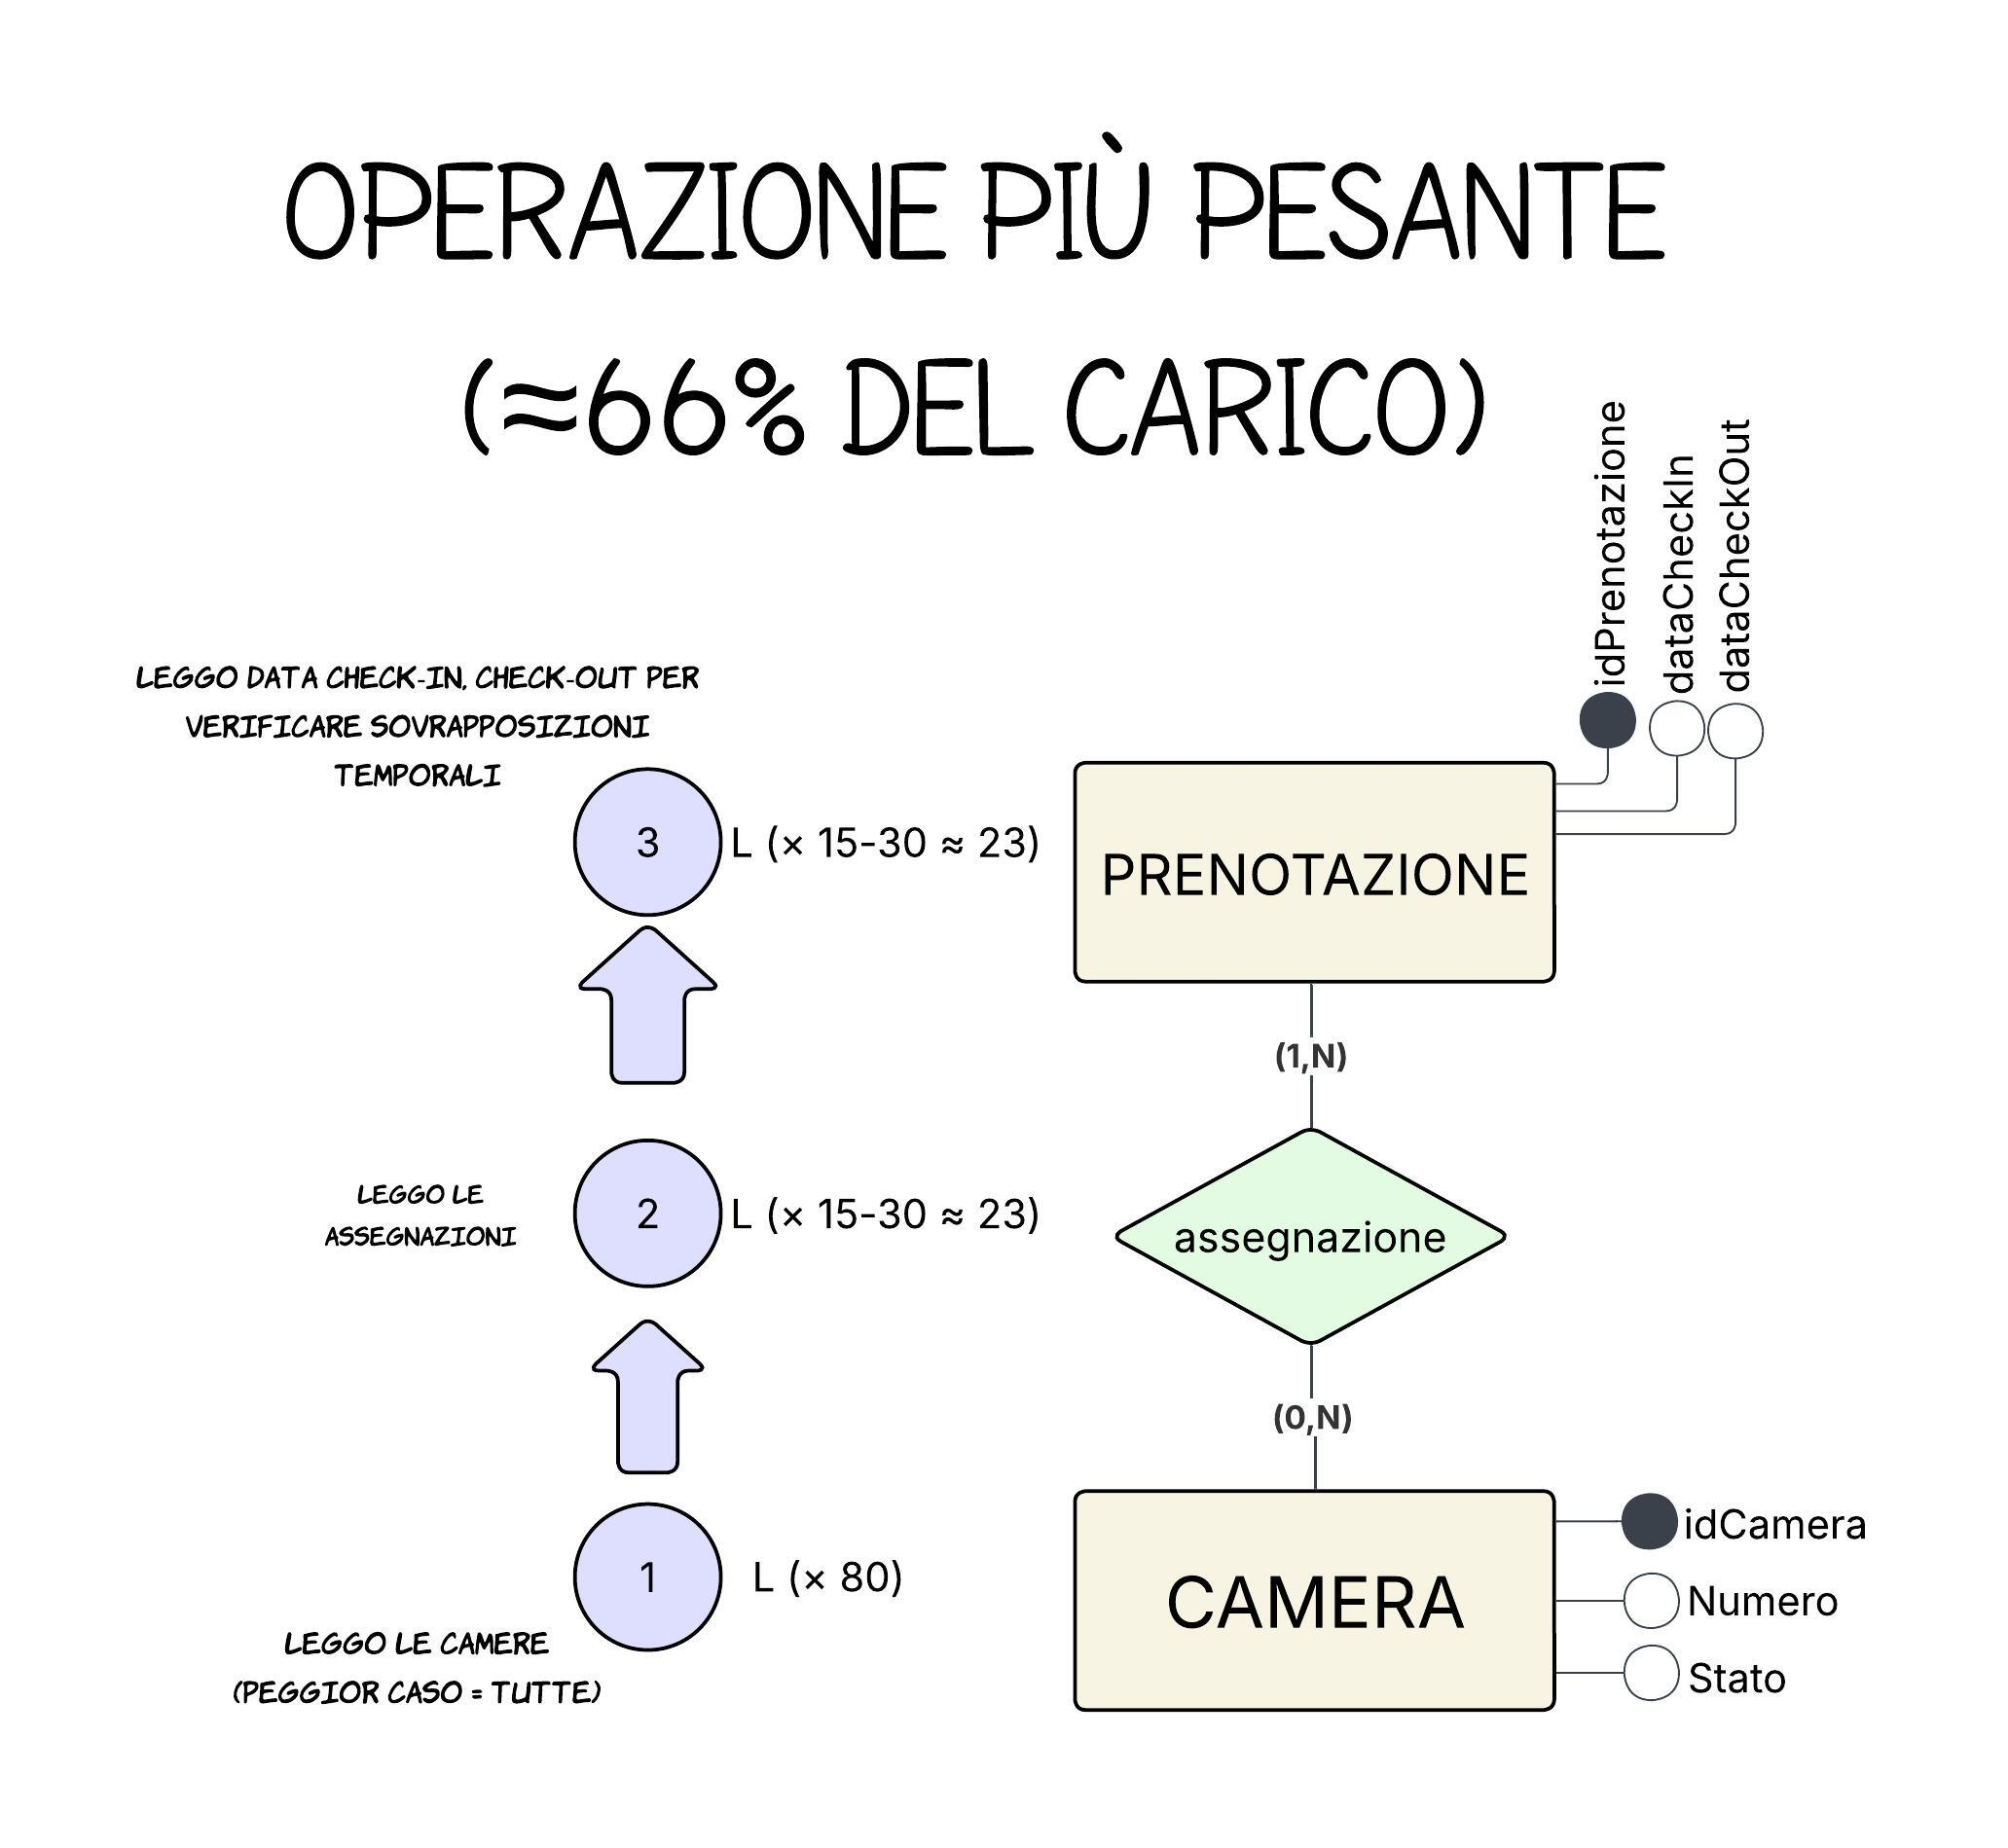
\includegraphics[width=0.55\textwidth]{../resources/nav/HotelDB_Nav_ConsultaDisponibilita.jpeg}
    \caption{Schema di navigazione --- Consulta disponibilità camere}
\end{figure}

\begin{table}[H]
    \centering
    \rowcolors{2}{gray!10}{white}
    \begin{tabular}{|l|c|c|c|}
        \hline
        \rowcolor{headerblue}
        \textbf{Concetto} & \textbf{Costrutto} & \textbf{Accessi}                  & \textbf{Tipo}    \\
        \hline
        CAMERA            & E                  & 80                                & L                \\
        ASSEGNAZIONE      & A                  & \textasciitilde{}15-30            & L                \\
        PRENOTAZIONE      & E                  & \textasciitilde{}15-30            & L                \\
        \hline
        \rowcolor{gray!25}
        \textbf{Totale}   &                    & \textbf{\textasciitilde{}110-140} & \textbf{tutti L} \\
        \hline
    \end{tabular}
    \caption{Tavola degli accessi --- Consulta disponibilità camere}
\end{table}

Costo giornaliero dell'operazione $\approx 126 \times 50 \approx 6.300$
accessi/giorno (range 5.500--7.000 a seconda della distribuzione
temporale reale delle prenotazioni). Come verrà riportato in
\cref{sec:sintesiCarico}, questa singola operazione domina il carico
complessivo del sistema pur avendo una frequenza (50/g) tutt'altro che
estrema: è il caso più chiaro di ``costo per accesso alto $\times$
frequenza moderata = carico totale dominante''.

\subsection{Consulta prenotazioni per data}
\label{sec:ConsultaPrenotazioniData}

Il report richiesto (relazione, Requisiti funzionali --- Reportistica) è
la lista delle \textbf{prenotazioni} con soggiorno attivo in una data
specifica, o in un intervallo se richiesto: il filtro è quindi
sulla \textbf{sovrapposizione temporale} tra
[\texttt{dataCheckIn}, \texttt{dataCheckOut}) e la data/intervallo
richiesti, non sul solo \texttt{dataCheckIn}. Si tratta dello stesso tipo
di interrogazione già analizzato in
\cref{sec:ConsultaDisponibilita} (sovrapposizione di intervalli), qui
applicata nel verso opposto: lì si cercano le camere \emph{non} coinvolte
in prenotazioni sovrapposte, qui si cercano direttamente le prenotazioni
sovrapposte. Si riusa quindi la stessa assunzione statistica --- 15--30
righe coinvolte, punto medio $\approx$23 --- anziché il tasso di nuove
prenotazioni giornaliere usato in una prima stima poi rivista.

\textit{Nota sullo scope}: il risultato è un elenco di prenotazioni, non
di camere; la vista ``camere occupate in un intervallo'' non è tra i
report richiesti (relazione, requisiti funzionali) e non viene quindi
modellata come operazione separata, per non introdurre complessità non
richiesta (Regola 3). Poiché non esiste un attributo
\textit{StatoAttuale} su \textbf{PRENOTAZIONE}, per mostrare lo stato di
ciascuna prenotazione occorre risalire alla riga più recente di
\textbf{VARIAZIONE} per ciascuna, assistita da un indice su
(\texttt{idPrenotazione}, \texttt{DataOraCambio}). Si assume, come
default, che vengano mostrate le prenotazioni indipendentemente dal loro
stato (compresa una eventuale ``Cancelled''), lasciando alla colonna
stato la distinzione visiva --- da confermare se invece va escluso un
sottoinsieme di stati.

\begin{figure}[H]
    \centering
    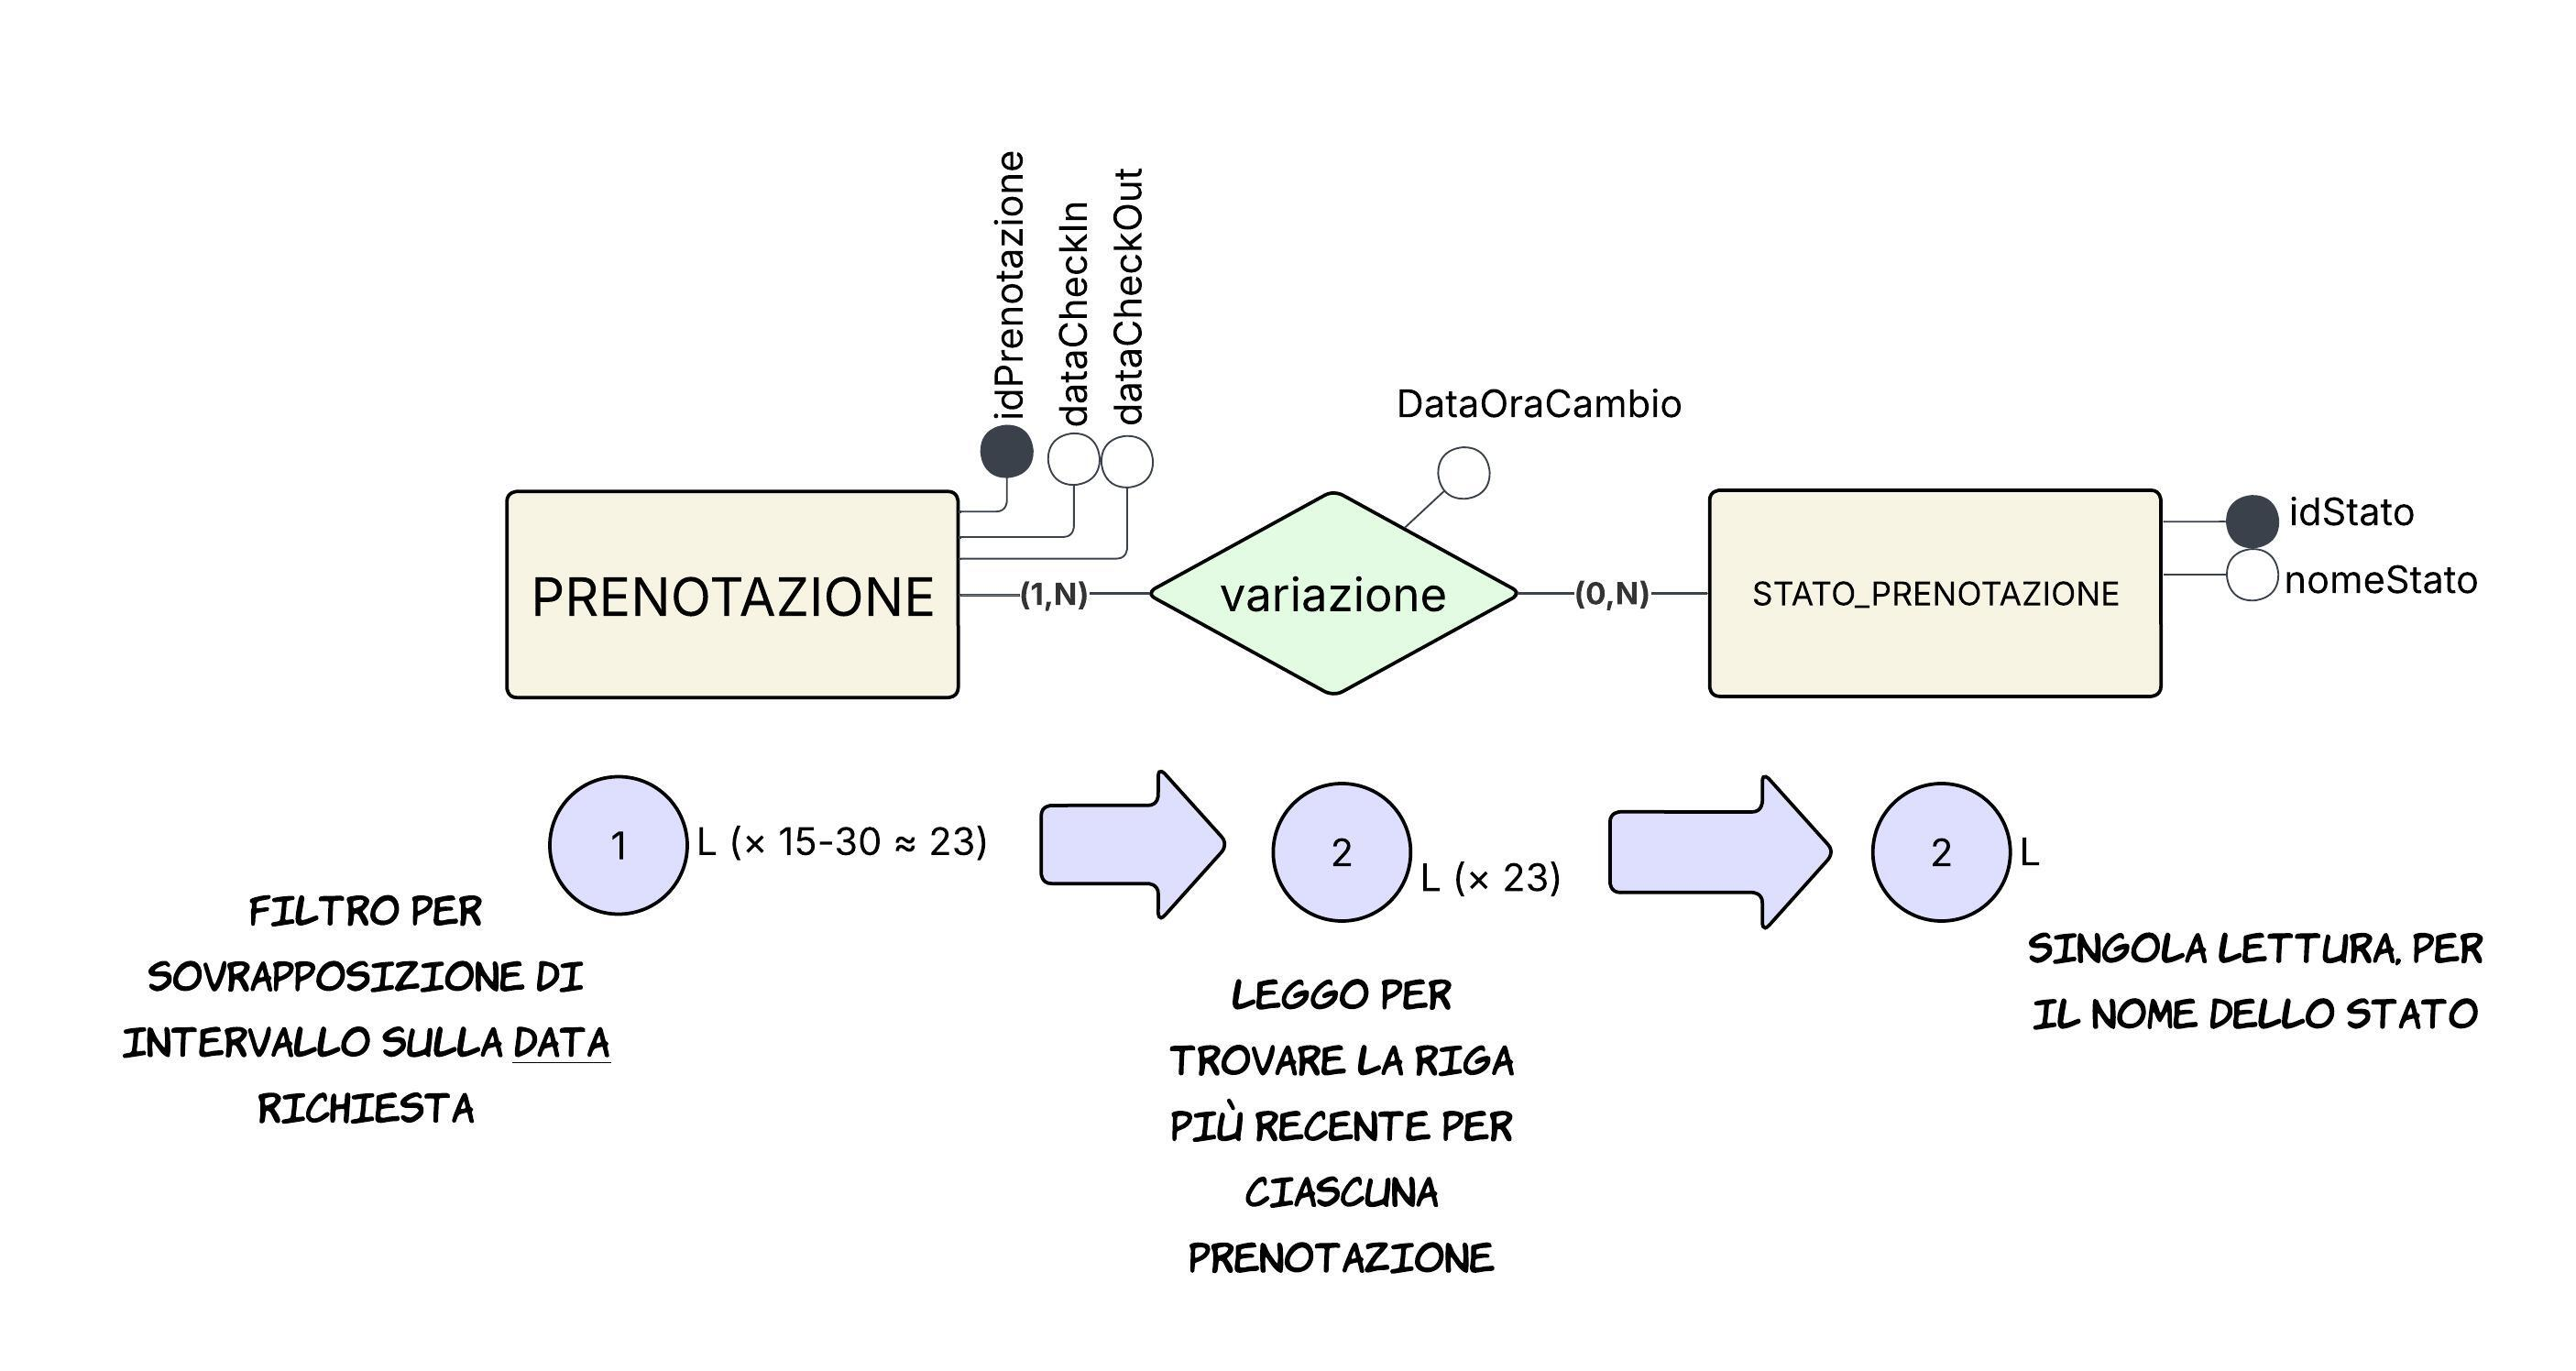
\includegraphics[width=0.55\textwidth]{../resources/nav/HotelDB_Nav_ConsultaPrenotazioniData.jpeg}
    \caption{Schema di navigazione --- Consulta prenotazioni per data}
\end{figure}

\begin{table}[H]
    \centering
    \rowcolors{2}{gray!10}{white}
    \begin{tabular}{|l|c|c|c|}
        \hline
        \rowcolor{headerblue}
        \textbf{Concetto}   & \textbf{Costrutto} & \textbf{Accessi}             & \textbf{Tipo}    \\
        \hline
        PRENOTAZIONE        & E                  & \textasciitilde{}15-30 (23)  & L                \\
        VARIAZIONE          & A                  & \textasciitilde{}15-30 (23)  & L                \\
        STATO\_PRENOTAZIONE & E                  & 1                            & L                \\
        \hline
        \rowcolor{gray!25}
        \textbf{Totale}     &                    & \textbf{\textasciitilde{}47} & \textbf{tutti L} \\
        \hline
    \end{tabular}
    \caption{Tavola degli accessi --- Consulta prenotazioni per data}
\end{table}

Costo giornaliero dell'operazione $\approx 47 \times 10 \approx 470$
accessi/giorno. Per una richiesta su intervallo (anziché giorno singolo)
il numero di prenotazioni coinvolte può crescere con l'ampiezza
dell'intervallo; in assenza di un'assunzione sulla distribuzione più
precisa, si mantiene questa stima come caso base, da rivedere se in fase
di test emergano intervalli tipici molto ampi.

\subsection{Assegna ruolo a utente}
\label{sec:AssegnaRuolo}

Inserisce una riga in \textbf{ATTRIBUZIONE}. Frequenza dichiarata in
\cref{tab:operazioni} come 2/mese; per coerenza con le altre tavole si
converte in $2/30 \approx 0{,}07$/giorno.

\begin{figure}[H]
    \centering
    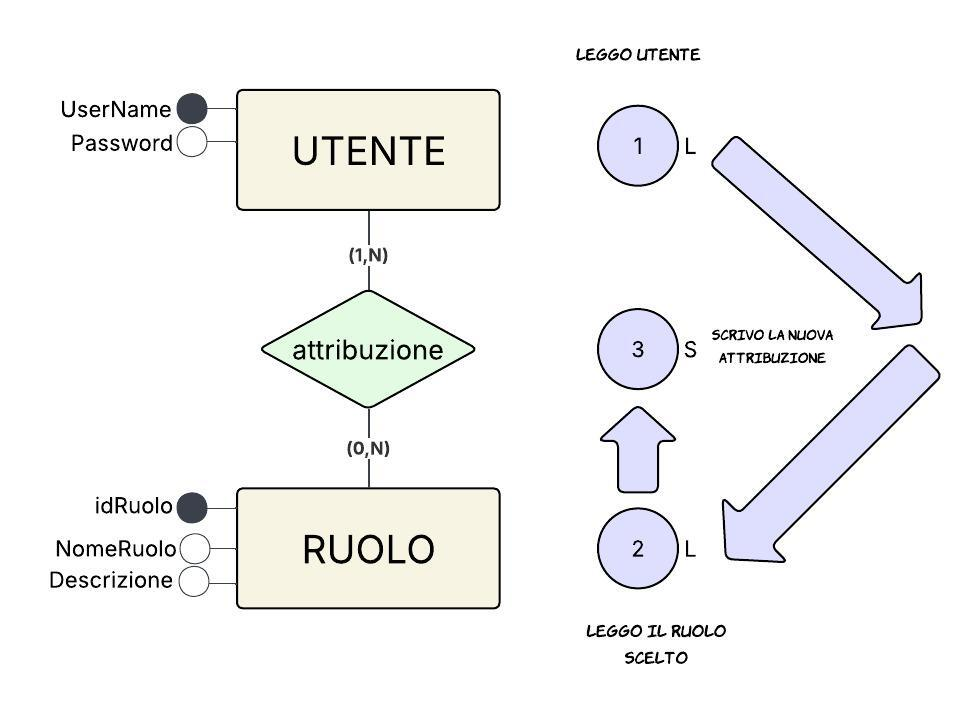
\includegraphics[width=0.55\textwidth]{../resources/nav/HotelDB_Nav_AssegnaRuolo.jpeg}
    \caption{Schema di navigazione --- Assegna ruolo a utente}
\end{figure}

\begin{table}[H]
    \centering
    \rowcolors{2}{gray!10}{white}
    \begin{tabular}{|l|c|c|c|}
        \hline
        \rowcolor{headerblue}
        \textbf{Concetto} & \textbf{Costrutto} & \textbf{Accessi} & \textbf{Tipo}    \\
        \hline
        UTENTE            & E                  & 1                & L                \\
        RUOLO             & E                  & 1                & L                \\
        ATTRIBUZIONE      & A                  & 1                & S                \\
        \hline
        \rowcolor{gray!25}
        \textbf{Totale}   &                    & \textbf{3}       & \textbf{2L + 1S} \\
        \hline
    \end{tabular}
    \caption{Tavola degli accessi --- Assegna ruolo a utente}
\end{table}

Costo giornaliero dell'operazione $\approx (2L + 1S{\times}2) \times
    0{,}07 \approx 0{,}3$ accessi/giorno --- trascurabile, coerente con il
volume totale di sole 22 istanze di \textbf{ATTRIBUZIONE} stimate.

\subsection{Crea/modifica tipologia camera}
\label{sec:TipologiaCameraOp}

Configurazione quasi statica (frequenza dichiarata ``rara''). Si
modella il caso più oneroso (modifica: lettura seguita da scrittura).
\smallskip
\newline
\textit{Nota}: in assenza di un valore numerico nella tavola delle
operazioni, si adotta una stima puramente simbolica di
$\sim$1/mese ($\approx$0,03/giorno) al solo scopo di includerla nella
sintesi comparativa finale --- il valore esatto non altera la
conclusione, perché il carico resta comunque trascurabile per qualunque
cifra ragionevole.

\begin{table}[H]
    \centering
    \rowcolors{2}{gray!10}{white}
    \begin{tabular}{|l|c|c|c|}
        \hline
        \rowcolor{headerblue}
        \textbf{Concetto} & \textbf{Costrutto} & \textbf{Accessi} & \textbf{Tipo}    \\
        \hline
        TIPOLOGIA\_CAMERA & E                  & 1                & L                \\
        TIPOLOGIA\_CAMERA & E                  & 1                & S                \\
        \hline
        \rowcolor{gray!25}
        \textbf{Totale}   &                    & \textbf{2}       & \textbf{1L + 1S} \\
        \hline
    \end{tabular}
    \caption{Tavola degli accessi --- Crea/modifica tipologia camera}
\end{table}

Costo giornaliero (stimato) $\approx 0{,}1$ accessi/giorno.

\subsection{Crea/modifica servizio accessorio}
\label{sec:ServizioOp}

Stessa struttura e stessa nota metodologica dell'operazione precedente,
applicata a \textbf{SERVIZIO}.

\begin{table}[H]
    \centering
    \rowcolors{2}{gray!10}{white}
    \begin{tabular}{|l|c|c|c|}
        \hline
        \rowcolor{headerblue}
        \textbf{Concetto} & \textbf{Costrutto} & \textbf{Accessi} & \textbf{Tipo}    \\
        \hline
        SERVIZIO          & E                  & 1                & L                \\
        SERVIZIO          & E                  & 1                & S                \\
        \hline
        \rowcolor{gray!25}
        \textbf{Totale}   &                    & \textbf{2}       & \textbf{1L + 1S} \\
        \hline
    \end{tabular}
    \caption{Tavola degli accessi --- Crea/modifica servizio accessorio}
\end{table}

Costo giornaliero (stimato) $\approx 0{,}1$ accessi/giorno.

\subsection{Calcola fatturato giornaliero}
\label{sec:FatturatoGiornaliero}

Operazione batch notturna: aggrega ricavi da prenotazioni concluse
(check-out avvenuto nella giornata) e consumazioni registrate nella
giornata. Poiché \textbf{PRENOTAZIONE} non ha un attributo di prezzo
totale, il ricavo camera va ricostruito per ogni prenotazione conclusa
tramite \textbf{ASSEGNAZIONE} $\to$ \textbf{CAMERA} $\to$
\textbf{TIPOLOGIA\_CAMERA} (× \texttt{PrezzoBase}), applicando lo
sconto loyalty corrente. Si stima il numero di check-out giornalieri pari al
tasso medio di nuove prenotazioni ($\approx$23/g, assumendo che quasi
ogni prenotazione arrivi infine a check-out). Il numero di consumazioni
giornaliere ($\approx$183) riusa direttamente la stima già validata in
\cref{sec:RegistraConsumazione}.
\iffalse
    \begin{figure}[H]
        \centering
        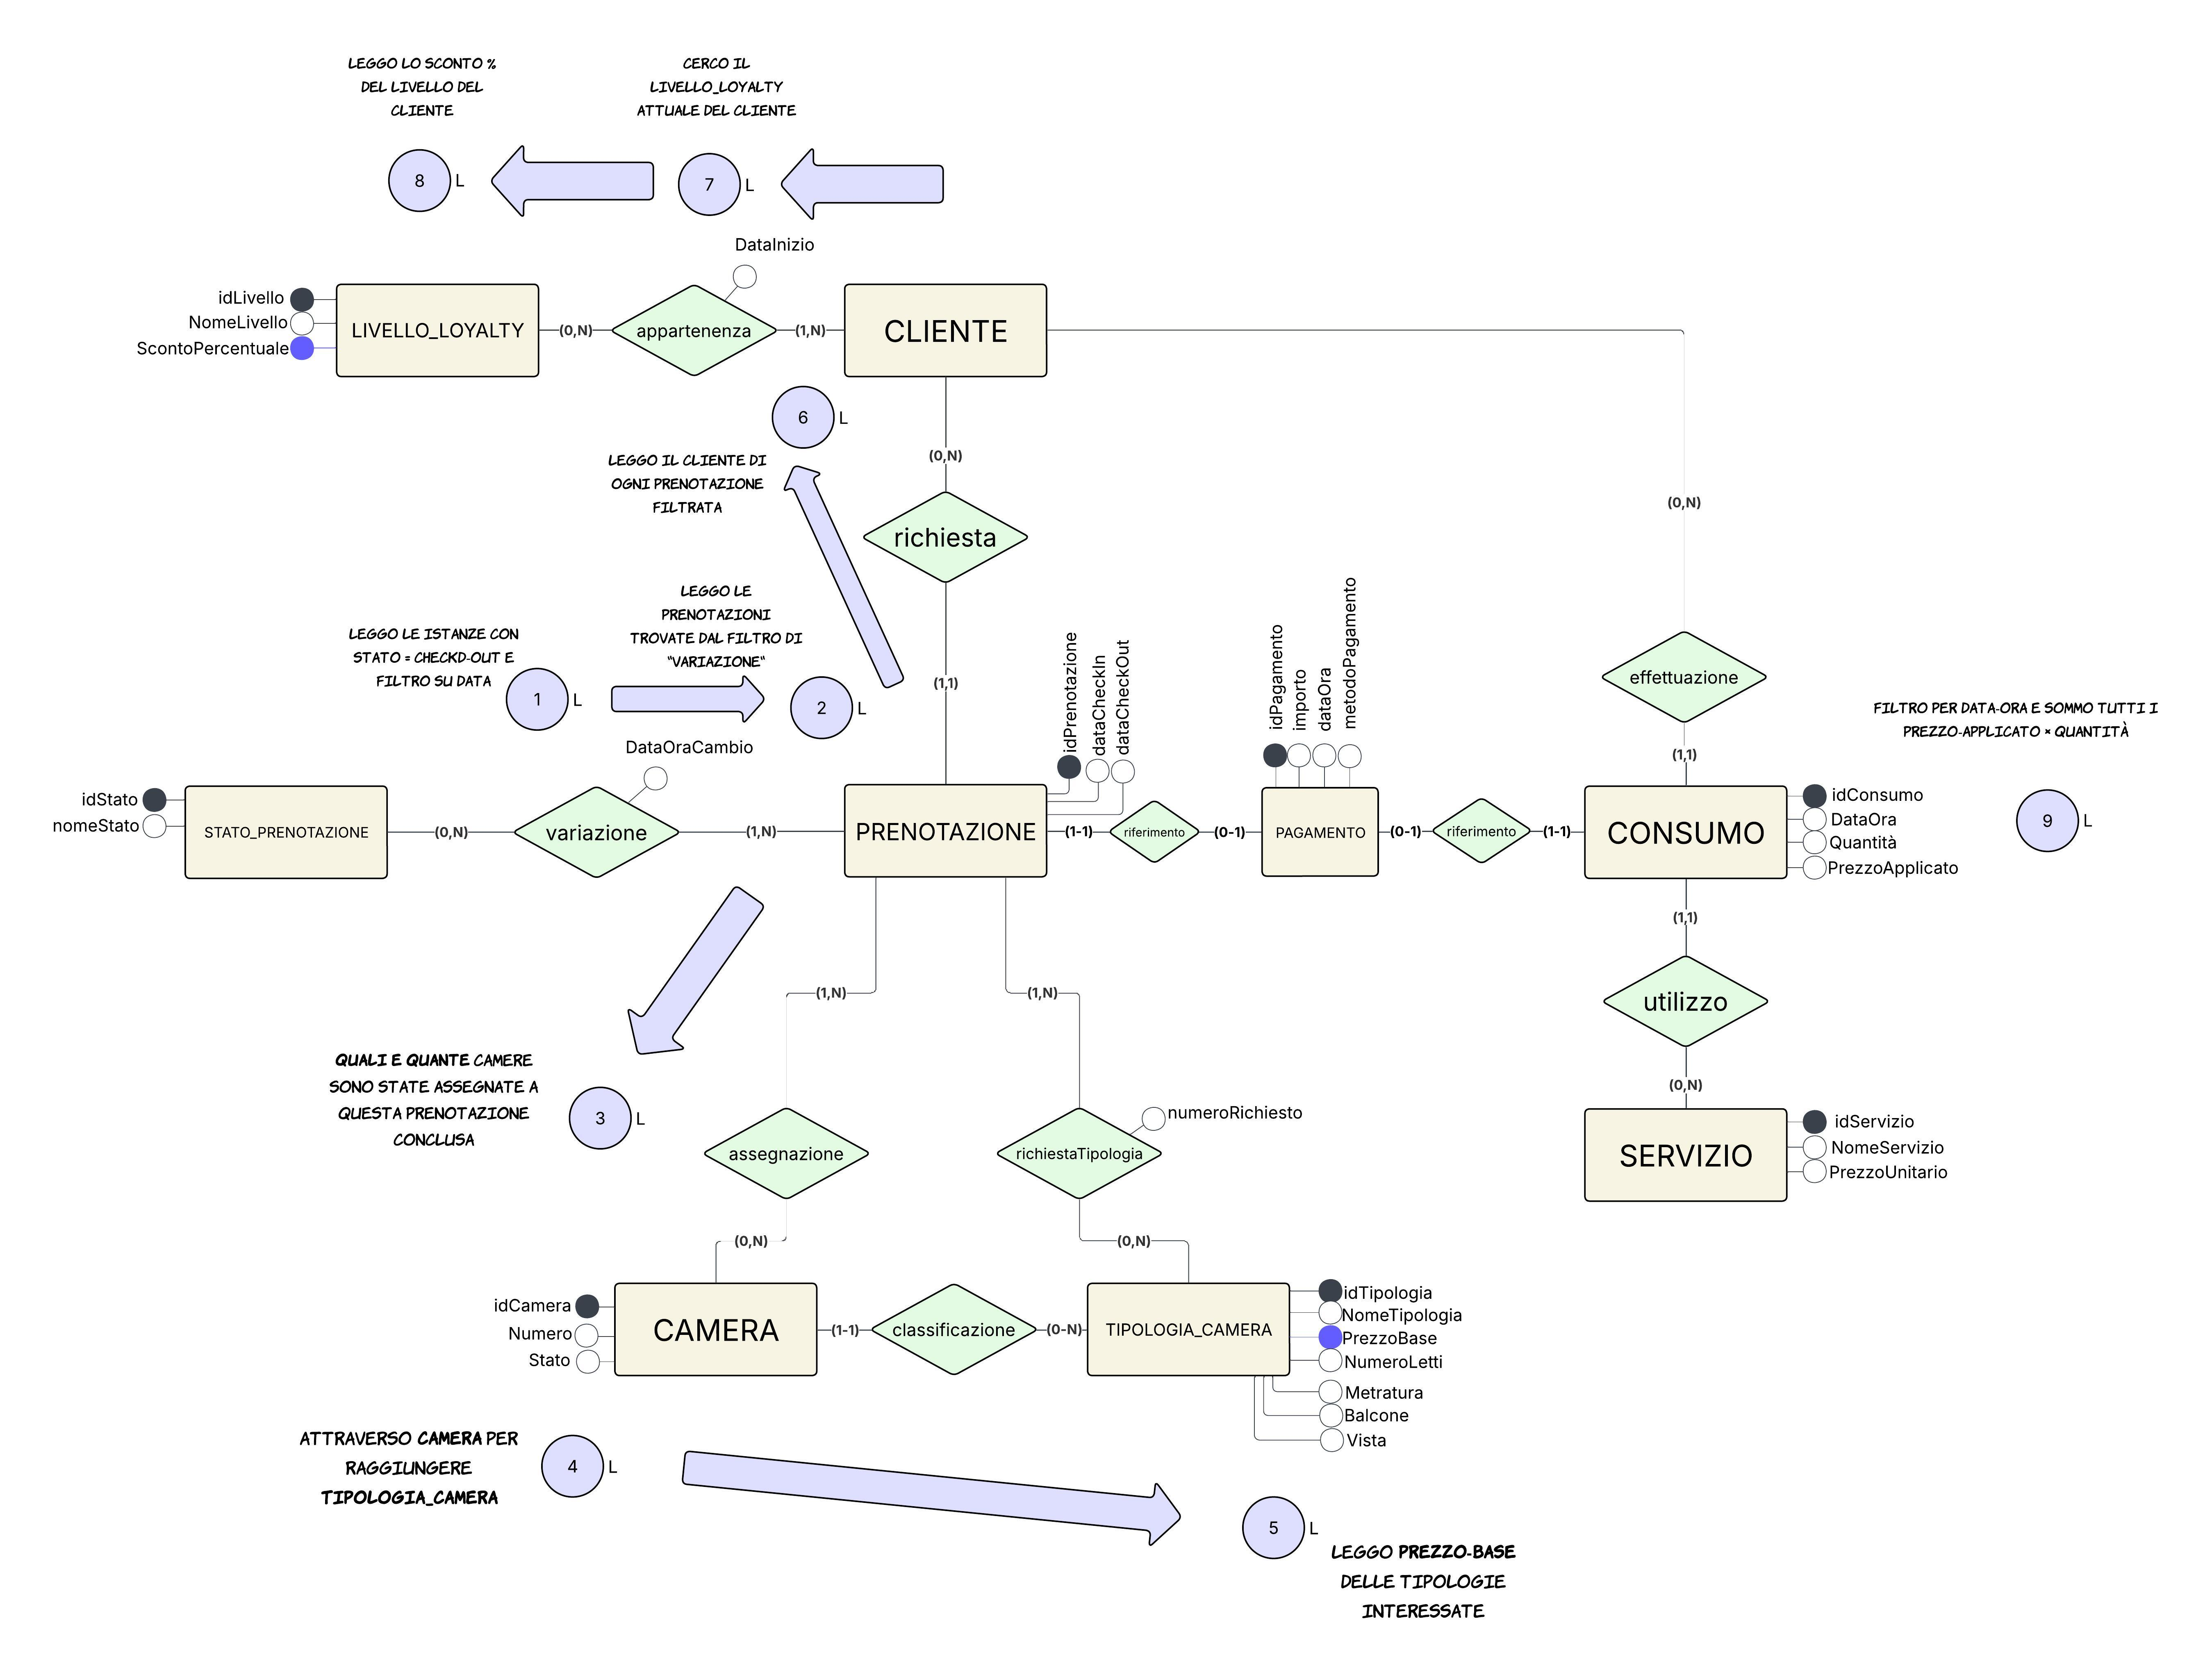
\includegraphics[width=0.65\textwidth]{../resources/nav/HotelDB_Nav_FatturatoGiornaliero.jpeg}
        \caption{Schema di navigazione --- Calcola fatturato giornaliero}
    \end{figure}
\fi
\begin{table}[H]
    \centering
    \rowcolors{2}{gray!10}{white}
    \begin{tabular}{|l|c|c|c|}
        \hline
        \rowcolor{headerblue}
        \textbf{Concetto} & \textbf{Costrutto} & \textbf{Accessi}              & \textbf{Tipo}    \\
        \hline
        VARIAZIONE        & A                  & \textasciitilde{}23           & L                \\
        PRENOTAZIONE      & E                  & \textasciitilde{}23           & L                \\
        ASSEGNAZIONE      & A                  & \textasciitilde{}32           & L                \\
        CAMERA            & E                  & \textasciitilde{}32           & L                \\
        TIPOLOGIA\_CAMERA & E                  & \textasciitilde{}32           & L                \\
        CLIENTE           & E                  & \textasciitilde{}23           & L                \\
        APPARTENENZA      & A                  & \textasciitilde{}30           & L                \\
        LIVELLO\_LOYALTY  & E                  & \textasciitilde{}23           & L                \\
        CONSUMO           & E                  & \textasciitilde{}183          & L                \\
        \hline
        \rowcolor{gray!25}
        \textbf{Totale}   &                    & \textbf{\textasciitilde{}401} & \textbf{tutti L} \\
        \hline
    \end{tabular}
    \caption{Tavola degli accessi --- Calcola fatturato giornaliero}
\end{table}

Costo giornaliero dell'operazione $\approx 401 \times 1 = 401$
accessi/giorno. È un contrasto istruttivo con \textit{Consulta
    disponibilità}: qui il costo \emph{per esecuzione} è il più alto di
tutta la tavola, ma la frequenza minima (1/g, essendo un batch notturno)
lo rende comunque secondario nel carico complessivo del sistema.

\subsection{Calcola incassi giornalieri}
\label{sec:IncassiGiornalieri}

Operazione batch notturna complementare a "Calcola fatturato
giornaliero".
\newline
Mentre \texttt{CalcolaFatturato} analizza il fatturato \emph{per
    competenza} (erogazione del servizio), \texttt{CalcolaIncassi}, misura gli incassi
\emph{per cassa}, ovvero quelli effettivamente entrati in quella data.
\newline
Nell'effettivo aggrega l'
\texttt{Importo} di tutti i \textbf{PAGAMENTO} con \texttt{DataOra}
pari al giorno corrente in un unico valore. Si stima il numero di pagamenti giornalieri
pari alla somma dei pagamenti contestuali generati da \textit{Crea
    prenotazione} ($\approx$23/g) e da \textit{Registra consumazione
    servizio} ($\approx$183/g), $\approx$ 206/g.

\begin{table}[H]
    \centering
    \rowcolors{2}{gray!10}{white}
    \begin{tabular}{|l|c|c|c|}
        \hline
        \rowcolor{headerblue}
        \textbf{Concetto} & \textbf{Costrutto} & \textbf{Accessi}              & \textbf{Tipo}    \\
        \hline
        PAGAMENTO         & E                  & \textasciitilde{}206          & L                \\
        \hline
        \rowcolor{gray!25}
        \textbf{Totale}   &                    & \textbf{\textasciitilde{}206} & \textbf{tutti L} \\
        \hline
    \end{tabular}
    \caption{Tavola degli accessi --- Calcola incassi giornalieri}
\end{table}

Costo giornaliero dell'operazione $\approx 206 \times 1 = 206$
accessi/giorno.

\subsection{Sintesi del carico giornaliero e individuazione delle operazioni critiche}
\label{sec:sintesiCarico}

Con il costo giornaliero calcolato per tutte le operazioni, si applica
ora la regola 80-20 su dati completi anziché su una selezione a priori.

\begin{table}[H]
    \centering
    \rowcolors{2}{gray!10}{white}
    \small
    \begin{tabular}{|p{6.2cm}|c|c|}
        \hline
        \rowcolor{headerblue}
        \textbf{Operazione}               & \textbf{Accessi/g}             & \textbf{\% cumulata} \\
        \hline
        Consulta disponibilità camere     & 6.300                          & 66,3\%               \\
        Registra consumazione servizio    & 1098                           & 77,8\%               \\
        Consulta prenotazioni per data    & 470                            & 82,8\%               \\
        Calcola fatturato giornaliero     & 401                            & 87,0\%               \\
        Cambia stato prenotazione         & 368                            & 90,8\%               \\
        Crea prenotazione                 & 237                            & 93,3\%               \\
        Calcola incassi giornalieri       & 206                            & 95,5\%               \\
        Assegna camera/e a prenotazione   & 166                            & 97,2\%               \\
        Aggiorna stato camera             & 138                            & 98,7\%               \\
        Assegna livello loyalty a cliente & 68                             & 99,4\%               \\
        Registra nuovo cliente            & 56                             & 100,0\%              \\
        Assegna ruolo a utente            & 0,3                            & 100,0\%              \\
        Crea/modifica tipologia camera    & 0,1                            & 100,0\%              \\
        Crea/modifica servizio accessorio & 0,1                            & 100,0\%              \\
        \hline
        \rowcolor{gray!25}
        \textbf{Totale sistema}           & \textbf{\textasciitilde{}9508} &                      \\
        \hline
    \end{tabular}
    \caption{Carico giornaliero complessivo per operazione, in ordine decrescente}
    \label{tab:sintesiCarico}
\end{table}

Applicando rigorosamente la regola 80-20: le prime \textbf{tre}
operazioni (\textit{Consulta disponibilità camere},
\textit{Registra consumazione servizio}, \textit{Consulta prenotazioni
    per data}) coprono da sole l'82,8\% del carico giornaliero complessivo del
sistema, pur essendo solo 3 delle 14 operazioni analizzate. Questo
conferma quantitativamente quanto già osservato qualitativamente in
precedenza su \textit{Consulta disponibilità camere}, ma la ridimensiona
correttamente: da sola pesa per il 66,3\% del carico totale, un ordine di
grandezza sopra qualunque altra operazione.

\chapter{Progettazione dell'Applicazione}

% Da completare quando si arriva a questa fase del progetto:
% - Architettura del software
% - Screenshot dell'interfaccia utente

\end{document}
